\documentclass[12pt]{article}
\setlength{\headheight}{35pt} 

%----------------------------------------------------------
% Packages
%----------------------------------------------------------
\usepackage[vmargin=1.18in,hmargin=1.1in]{geometry}				% page layout
\usepackage{amssymb,amsfonts,amsthm,mathtools,bm,bbm,mathrsfs} 	% math fonts/symbols
\usepackage[dvipsnames]{xcolor} 								% for \textcolor
\usepackage[colorlinks, linkcolor = blue, citecolor = blue, urlcolor = blue]{hyperref} 								% for hyperlinks 
\usepackage{graphicx} 											% for \includegraphics
\usepackage{caption} 											% for figure and table captions
\usepackage{verbatim}
\usepackage[misc]{ifsym} 										% for \Letter
\usepackage[ruled, linesnumbered]{algorithm2e} 					% for algorithm box
\usepackage{layouts} % to get information about document layout
\usepackage[uniquename=false, 
			uniquelist = false, 
			url = false, 
			doi = false, 
			isbn = false, 
			natbib = true, 
			backend = bibtex, 
			style = authoryear, 
			maxbibnames = 5]{biblatex} 							% for citations and bibliography
% \RequirePackage{amsthm,amsmath,amsfonts,amssymb,mathtools,bm,bbm,mathrsfs}  % typesetting                                    % author-year citations
% \RequirePackage[colorlinks,citecolor=blue,urlcolor=blue]{hyperref}          % coloring bibliography citations and linked URLs                                        
% \RequirePackage{verbatim}
% \RequirePackage[ruled, linesnumbered]{algorithm2e} 					        % for algorithm box
\usepackage{booktabs} % to make book table
\usepackage{multirow} % to create table with multirow
\usepackage[noend]{algpseudocode}
\usepackage{subcaption}
\usepackage{multirow}

\geometry{a4paper,scale=0.75}

\newenvironment{breakablealgorithm}
{% \begin{breakablealgorithm}
	\begin{center}
		\refstepcounter{algorithm}% New algorithm
		\hrule height.8pt depth0pt \kern2pt% \@fs@pre for \@fs@ruled
		\renewcommand{\caption}[2][\relax]{% Make a new \caption
			{\raggedright\textbf{\ALG@name~\thealgorithm} ##2\par}%
			\ifx\relax##1\relax % #1 is \relax
			\addcontentsline{loa}{algorithm}{\protect\numberline{\thealgorithm}##2}%
			\else % #1 is not \relax
			\addcontentsline{loa}{algorithm}{\protect\numberline{\thealgorithm}##1}%
			\fi
			\kern2pt\hrule\kern2pt
		}
	}{% \end{breakablealgorithm}
		\kern2pt\hrule\relax% \@fs@post for \@fs@ruled
	\end{center}
}
\makeatother


\newcommand{\zn}[1]{\textcolor{purple}{[ZN: #1]}}
\newcommand{\ek}[1]{\textcolor{red}{[EK: #1]}}
\newcommand{\jrc}[1]{\textcolor{blue}{[JRC: #1]}}

\newtheorem{assumption}{Assumption}
\newtheorem{theorem}{Theorem}
\newtheorem{corollary}{Corollary}
\newtheorem{lemma}{Lemma}
\newtheorem{proposition}{Proposition}
\newtheorem{definition}{Definition}
\theoremstyle{definition}
\newtheorem{example}{Example}
\newtheorem{remark}{Remark}
\newcommand{\indep}{\perp \!\!\! \perp}


%%%%%%%%%%%%%%%%%%%%%%%%%%%%%%

\def\X{\bm{X}}
\def\mP{\mathbb{P}}
\def\A{\bm{A}}
\def\P{\mathbb{P}}
\def\iid{\mathrm{iid}}
\def\H{\mathcal{H}}
\def\Hk{\mathcal{H}_k}
\def\tht{\bm{\theta}}
\def\gama{\bm{\gamma}}
\def\Del{\bm{\Delta}}
\def\sgn{\mathrm{sgn}}
\def\P{\mathbb{P}}


%----------------------------------------------------------
% Generic macros
%----------------------------------------------------------
\newcommand{\E}{\mathbb E}								% expectation
\newcommand{\V}{\mathrm{Var}}							% variance
\renewcommand{\P}{\mathbb{P}}							% probability
\newcommand{\Q}{\mathbb{Q}}								% quantile
\newcommand{\R}{\mathbb{R}}								% reals
\newcommand{\Z}{\mathbb{Z}}								% integers
\newcommand{\N}{\mathbb{N}}								% naturals
\newcommand{\indicator}{\mathbbm 1}						% indicator
\newcommand{\norm}[1]{\left\lVert{#1}\right\rVert}		% norm
\newcommand{\independent}{{\perp \! \! \! \perp}}		% independent
\newcommand{\iidsim}{\stackrel{\mathrm{i.i.d.}}{\sim}} 	% i.i.d. distributed
\newcommand{\indsim}{\stackrel{\mathrm{ind}}{\sim}}		% independently distributed
\newcommand{\expit}{\mathrm{expit}}                 	% link function for logistic model
\newcommand{\convp}{\overset{\mathbb{P}}{\rightarrow}}             % convergence in probability
\newcommand{\convd}{\overset d \rightarrow}             % convergence in distribution
\newcommand{\convas}{\overset {a.s.} \rightarrow}       % convergence almost surely
\newcommand{\argmin}[1]{\underset{#1}{\arg \min}}       % arg min
\newcommand{\argmax}[1]{\underset{#1}{\arg \max}}       % arg max

%----------------------------------------------------------
% Paper-specific macros
%----------------------------------------------------------
\newcommand{\prx}{\bm X}								% population random X
\newcommand{\srx}{X}									% sample random X
\newcommand{\prz}{\bm Z}								% population random Z
\newcommand{\srz}{Z}									% sample random Z 
\newcommand{\prxk}{{{\widetilde{\bm X}}}}      			% population random resampled X
\newcommand{\seta}{s^{2}(\eta_0)}
\newcommand{\srxk}{\widetilde X}						% sample random resampled X
\newcommand{\pry}{{\bm Y}}								% population random Y
\newcommand{\sry}{Y}									% sample random Y 
\newcommand{\peps}{\bm \epsilon}						% population epsilon
\newcommand{\seps}{\epsilon}							% sample epsilon
\newcommand{\smu}{\mu}									% sample mu
\newcommand{\pmu}{\bm \mu}								% population mu
\newcommand{\law}{\mathcal L}							% law of (X,Y,Z)
\newcommand{\nulllaws}{\mathscr L^0}					% collection of null distributions
\newcommand{\regclass}{\mathscr R}					    % collection of distributions with regularity
\newcommand{\lawhat}{\widehat{\mathcal L}}				% estimated law of (X,Y,Z)
\newcommand{\CRT}{\textnormal{CRT}}             		% CRT
\newcommand{\dCRT}{\textnormal{dCRT}} 					% dCRT
\newcommand{\GCM}{\textnormal{GCM}}						% GCM
\newcommand{\dCRThat}{\widehat{\textnormal{dCRT}}}		% dCRT-hat
\newcommand{\MXtwohat}{\widehat{\textnormal{MX(2)}}}		% dCRT-hat
\newcommand{\ndCRThat}{\textnormal{ndCRT}}	% normalized dCRT-hat
\newcommand{\CRThat}{\widehat{\textnormal{CRT}}}		% CRT-hat
\renewcommand{\H}{\mathcal H}		 					% Hilbert subspace
\newcommand{\MXtwo}{\textnormal{MX(2)}}                 % MX(2)
\newcommand{\convdp}{\overset {d,p} \longrightarrow}    % conditional convergence in distribution
\newcommand{\convpp}{\overset {p,p} \longrightarrow}    % conditional convergence in probability
\newcommand{\spacrt}{\textnormal{spaCRT}}               % spaCRT
\newcommand{\aux}{\textnormal{aux}}               % auxiliary test
\newcommand{\asy}{\textnormal{asy}}              % asymptotic test
%----------------------------------------------------------
% Other macros
%----------------------------------------------------------
\let\oldnl\nl% Store \nl in \oldnl
\newcommand{\nonl}{\renewcommand{\nl}{\let\nl\oldnl}} % Remove line number for one line of alg

\addbibresource{spacrt.bib}
% \bibliography{spacrt.bib}


%%%%%%%%%%%%%%%%%%%%%%%%%%%%%%%%%%%%%%%%%%
\title{Computationally efficient and statistically accurate conditional independence testing with spaCRT}

\begin{document}

\author{Ziang Niu, Jyotishka Ray Choudhury, Eugene Katsevich}
\maketitle

\begin{abstract}
  We introduce the saddlepoint approximation-based conditional randomization test (spaCRT), a novel conditional independence test that effectively balances statistical accuracy and computational efficiency, inspired by applications to single-cell CRISPR screens. Resampling-based methods like the distilled conditional randomization test (dCRT) offer statistical precision but at a high computational cost. The spaCRT leverages a saddlepoint approximation to the resampling distribution of the dCRT test statistic, achieving very similar finite-sample statistical performance with significantly reduced computational demands. We prove that the spaCRT $p$-value approximates the dCRT $p$-value with vanishing relative error, and that these two tests are asymptotically equivalent. Through extensive simulations and real data analysis, we demonstrate that the spaCRT controls Type-I error and maintains high power, outperforming other asymptotic and resampling-based tests. Our method is particularly well-suited for large-scale single-cell CRISPR screen analyses, facilitating the efficient and accurate assessment of perturbation-gene associations.
\end{abstract}

\section{Introduction} \label{sec:introduction}

Motivated by applications to \textit{single-cell CRISPR screen} data analysis, we propose a resampling-free approximation to a resampling-based conditional independence test, the \textit{distilled conditional randomization test} (dCRT; \cite{Liu2022a}). In doing so, we arrive at a test that has the finite-sample statistical performance of a resampling-based procedure and the speed of an asymptotic test. 

\subsection{Motivating application: Single-cell CRISPR screens}

This work is motivated by the analysis of \textit{single-cell CRISPR screen} data \citep{Dixit2016,Adamson2016,Jaitin2016,Datlinger2017}. In these experiments, one of the biological objectives is to understand \textit{regulatory elements}, segments of DNA whose role is to control the expressions of one or more nearby genes. In particular, it is of interest to determine \textit{which} regulatory elements control the expressions of \textit{which} genes. This is a crucial question in understanding the genetic basis of human diseases, many of which are caused by genetic variants disrupting regulatory elements and therefore causing abnormal gene expression. To address this question, single-cell CRISPR screens are designed to subject a population of cells to a large number of \textit{CRISPR perturbations}, each of which inhibits the functioning of a specific regulatory element. Each cell receives several of these perturbations, and the expression of each gene in each cell is measured by single-cell RNA-sequencing. The statistical analysis task is to determine, for each CRISPR perturbation and gene of interest, whether cells with the perturbation have different gene expression levels compared to cells without the perturbation. To translate this into statistical language, let random variables $\prx \in \{0,1\}$, $\pry \in \N$, and $\prz \in \R^p$ represent the presence of a CRISPR perturbation, the gene expression level, and a set of covariates measured in a cell, respectively. The covariates $\prz$ include technical factors like library size (the total number of RNA molecules sequenced in a cell) and experimental batch, which may impact both $\prx$ and $\pry$ \citep{Katsevich2020c}. In the joint distribution $(\prx, \pry, \prz) \sim \law_n$ (potentially depending on the number of cells $n$), the statistical task is to test the null hypothesis 
\begin{equation}
H_0: \prx \indep \pry \mid \prz, 
\end{equation}
i.e., that the presence of the CRISPR perturbation is conditionally independent of the gene expression level, given the covariates. To this end, we collect observations $(\srx_{in}, \sry_{in}, \srz_{in}) \iidsim \law_n$ for cells $i = 1, \dots, n$. We denote these observations collectively as $\srx \in \R^n$, $\sry \in \R^n$, $\srz \in \R^{n \times p}$.

\subsection{Statistical and computational challenges} \label{sec:statistical-computational-challenges}

One challenging aspect of this problem is that both $\srx$ and $\sry$ are highly sparse. Indeed, due to the pooling of a large number of perturbations in a single experiment, most perturbations are present in only a small fraction of cells. Furthermore, gene expression data are measured as RNA molecule counts, and when measured at single-cell resolution, the relatively small number of total RNA molecules measured per cell and the large number of genes result in many genes having zero expression in most cells \citep{Svensson2020}. As a result, the effective sample size for testing $H_0$ is relatively small, which can cause asymptotic tests based on the central limit theorem to have inflated Type-I error rates \citep{Barry2024}. To address this challenge, we have proposed to apply the resampling-based \textit{conditional randomization test} (CRT; \cite{CetL16}). More specifically, we have employed an accelerated variant of the CRT called the dCRT \citep{Liu2022a}, coupled with a negative binomial regression-based test statistic, for single-cell CRISPR screen analysis \citep{Katsevich2020c}. The resulting method (SCEPTRE) and the associated R package (\verb|sceptre|) are considered the state of the art for perturbation-gene association testing in single-cell CRISPR screens, and have been employed in several recent studies \citep{Morris2021d,Tuano2023,Chardon2023a,Conery2024}.

Although the dCRT is much faster than the originally proposed variant of the CRT, it is still a resampling-based procedure, which poses computational challenges for large-scale applications like single-cell CRISPR screens. For example, \citet{Gasperini2019a} tested about 90,000 perturbation-gene pairs. Given the multiplicity correction required for such a large number of tests, $p$-values need to be accurate to about seven decimal places to have a chance at significance (assuming a Bonferroni correction at level $\alpha = 0.05$). Obtaining such accurate $p$-values requires about a million resamples per $p$-value, for a total of about $10^{12}$ resamples across all perturbation-gene pairs tested. Even with parallelization, this becomes quite a computationally intensive task. Therefore, we arrive at an apparent impasse: asymptotic methods are fast but inaccurate, while resampling-based methods are accurate but slow.

\subsection{Our contributions}

We propose a new method, the \textit{saddlepoint approximation-based conditional randomization test} ($\spacrt$), which reconciles the statistical accuracy of the dCRT with the computational efficiency of asymptotic methods. The key idea is to approximate the distribution of the resampled test statistic in the dCRT using a \textit{saddlepoint approximation} (SPA; \cite{Daniels1954,Lugannani1980}), a classical technique to obtain highly accurate approximations to densities and tail probabilities for quantities that can be expressed as sample averages. To preview the statistical and computational performance of the $\spacrt$, we present the analysis of the \citet{Gasperini2019a} single-cell CRISPR screen dataset (Figure~\ref{fig:dCRT_GCM_binomial_poisson}). In this analysis, we compare the $\spacrt$ to the generalized covariance measure (GCM) test \citep{Shah2018} (a conditional independence test based on asymptotic normality) and the dCRT using $M = 100,000$ resamples (for details on this analysis, see Section~\ref{sec:real_data}). We find that the $\spacrt$ is more than two orders of magnitude faster than the dCRT while maintaining Type-I error control, unlike the GCM test. We prove under relatively mild assumptions that the $\spacrt$ $p$-value has vanishing relative error compared to the $\dCRT$ $p$-value, and that the two tests are asymptotically equivalent. We demonstrate the statistical and computational advantages of the $\spacrt$ using extensive numerical simulations as well as an analysis of the \citet{Gasperini2019a} data. Code to reproduce these analyses is available at \href{https://github.com/Katsevich-Lab/spacrt-manuscript}{github.com/Katsevich-Lab/spacrt-manuscript}. 

\begin{figure*}[h!]
	\centering
	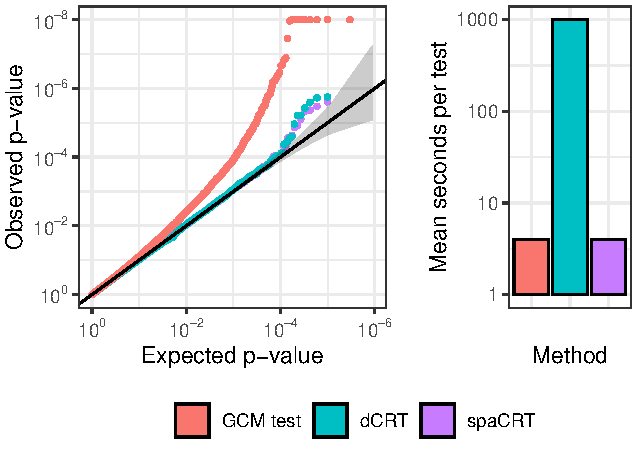
\includegraphics{figures-and-tables/motivating_example.pdf} 
	\caption{Comparing the Type-I error control and computation times of the $\GCM$ test, the $\dCRT$ and the proposed $\spacrt$ on the \citet{Gasperini2019a} data. {\color{red} We use logistic regression to model the perturbation $\prx|\prz$ and negative binomial regression to model the outcome $\pry|\prz$.} Left: QQ-plot of the $p$-values under the null hypothesis, obtained from testing 51 \textit{non-targeting} perturbations against 3,000 genes. The $p$-values are truncated from below at $10^{-8}$ for visualization purposes. Right: Mean computation times per perturbation-gene pair, in seconds.}
	\label{fig:dCRT_GCM_binomial_poisson} 
\end{figure*}

For single-cell CRISPR screen applications, the $\spacrt$ can be used to significantly accelerate the \verb|sceptre| software without compromising its statistical performance, facilitating the analysis of much larger datasets than previously possible. Beyond single-cell CRISPR screens, the conditional independence testing problem is a ubiquitous one, and the $\spacrt$ points the way towards a new class of fast and accurate tests.

\subsection{Related work}

In the same paper where the $\dCRT$ was introduced \citep{Liu2022a}, a resampling-free approximation to this procedure was proposed based on a quantile transformation to a normal distribution. However, these authors acknowledged that this approach is primarily useful for continuously distributed $\prx$, and that it incurs a substantial power loss for discrete $\prx$, the setting we are focused on in the present work. SPAs have been proposed to approximate resampling distributions of other resampling-based procedures, like permutation tests \citep{Robinson1982} and the bootstrap \citep{Hinkley1988}. However, to the best of our knowledge, the $\spacrt$ is the first application of SPA to a conditional independence test. Furthermore, existing applications of the SPA to resampling-based procedures have not been rigorously justified, a gap we address in a parallel work \citep{Niu2024}. In a different strand of work, resampling-based procedures have been accelerated using adaptive resampling schemes, which adjust the number of resamples drawn based on the data \citep{Besag1991,Gandy2009,Gandy2014,Gandy2016,Gandy2017a,Fischer2024a,Fischer2024}. Such procedures are applicable to arbitrary resampling schemes and test statistics, at the cost of some resampling. In contrast, the $\spacrt$ is a completely resampling-free procedure, though more specialized in its application.

\subsection{Outline of the paper}

We introduce the $\spacrt$ in Section~\ref{sec:spacrt}. We present the theoretical properties of the $\spacrt$ in Section~\ref{sec:theory}. We demonstrate the performance of the $\spacrt$ in a simulation study in Section~\ref{sec:simulation}. We apply the $\spacrt$ to the \citet{Gasperini2019a} data in Section~\ref{sec:real_data}. We conclude with a discussion in Section~\ref{sec:discussion}.

\subsection{Notation}

Define $\sgn(x)$ as the sign of $x$, i.e. $\sgn(x)=1$ if $x>0$, $-1$ if $x<0$ and $0$ otherwise. For an infinitely differentiable function $f:\mathcal{X}\subset\mathbb{R}\mapsto\mathbb{R}$, define $f^{(r)}$ to be its $r$-th derivative. Define $f',f''$ as the first and second derivative of $f$ respectively. Denote $[n]$ for any $n\in\mathbb{N}_+$ as $\{1,\ldots,n\}$. Define $\expit(x)\equiv 1/ (1+\exp(-x))$. Define $\E_{\law_n}[\cdot\mid\mathcal{F}_n],\E_{\lawhat_n}[\cdot\mid\mathcal{F}_n]$ as the conditional expectations under law $\law_n$ and its estimate $\lawhat_n$ respectively. Similarly, we define $\V_{\law_n}[\cdot\mid\mathcal{F}_n]$ and $\V_{\lawhat_n}[\cdot\mid\mathcal{F}_n]$ as the conditional variance counterpart. We use the following standard notations regarding the asymptotic properties of a sequence of random variables $X_n$:
\begin{align*}
  &X_n = O_{\P}(1) &&\text{ if for each } \delta > 0 \text{ there is an } M > 0 \text{ s.t. } \limsup_{n \rightarrow \infty}\P[|X_n| > M] < \delta; \\
  &X_n = \Omega_{\P}(1) &&\text{ if for each } \delta > 0 \text{ there is an } \eta > 0 \text{ s.t. } \limsup_{n \rightarrow \infty}\P[|X_n| < \eta] < \delta;\\
  &X_n = o_{\P}(1) &&\text{ if } \P[|X_n| > \eta] \rightarrow 0 \text{ for all } \eta > 0.
\end{align*}

\section{$\spacrt$: A resampling-free approximation to $\dCRT$} \label{sec:spacrt}

\subsection{Background: $\dCRT$}

The original dCRT procedure, as proposed by \citet{Liu2022a}, is designed under the \textit{model-X assumption} that $\law_n(\prx \mid \prz)$ is known \citep{CetL16}. However, this procedure is usually deployed in practice by learning this conditional distribution in-sample. In a prior work, we established the statistical properties of the dCRT with $\law_n(\prx \mid \prz)$ estimated in sample \citep{Niu2022a}. In this paper, we will refer to the latter procedure as the $\dCRT$, allowing a minor abuse of terminology. Furthermore, we consider the special case when 
\begin{equation}
\law_n(\prx \mid \prz) = f(\prx \mid \theta_{n,x}(\prz)), 
\end{equation}
where $f(x|\theta)$ is an exponential family with natural parameter $\theta$, natural parameter space $\R$, and log-partition function $A$:
\begin{align*}
f(x|\theta)=\exp(\theta x -A(\theta))h(x).
\end{align*}
This is not a restrictive assumption, since we allow the function $\theta_{n,x}(\prz)$ to be arbitrary. Given this setup, consider estimating the functions $\theta_{n,x}(\prz)$ and $\mu_{n,y}(\prz) \equiv \E_{\law_n}[\pry \mid \prz]$ by $\widehat{\theta}_{n,x}(\prz)$ and $\widehat \mu_{n,y}(\prz)$, respectively (we assume throughout that $\pry$ is integrable, so that $\mu_{n,y}$ is well-defined). The learning procedures for these quantities can be arbitrary. Setting $\widehat \mu_{n,x}(\prz) \equiv A'(\widehat{\theta}_{n,x}(\prz))$, we arrive at the test statistic 
\begin{align}\label{eq:dCRThat}
	T_n^{\dCRT}(X,Y,Z)
  =\frac{1}{n}\sum_{i=1}^{n}(\srx_{in}-\widehat\mu_{n,x}(\srz_{in}))(\sry_{in}-\widehat{\mu}_{n,y}(\srz_{in})).
\end{align}
The $\dCRT$ is obtained by comparing $T_n^{\dCRT}(\srx, \sry, \srz)$ to a null distribution obtained by resampling $\srx_{in} \mid \srz_{in}$ based on the estimated distribution $f(\cdot \mid \widehat \theta_{n,x}(Z_{in})).$ This procedure is summarized in Algorithm \ref{alg:dcrt-hat}. 

{\color{red}
The $\dCRT$ (Algorithm \ref{alg:dcrt-hat}) has many desirable statistical properties which make it a suitable choice for testing conditional independence. First, it is a resampling-based test and thus can potentially improve finite-sample performance compared to its asymptotic counterpart, the GCM test, which relies on asymptotic normality. While this improvement is quite evident in practice (recall Figure~\ref{fig:dCRT_GCM_binomial_poisson}), the theoretical basis for this improvement has not yet been established; this interesting research direction is beyond the scope of the current work. Moreover, the $\dCRT$ allows flexible in modeling choices: the estimator $\widehat{\mu}_{n,y}(\cdot)$ of the conditional expectation $\E[\pry\mid\prz=\cdot]$ can be constructed by any regression method. The choices include but are not limited to parametric, non-parametric and high-dimensional regression methods. Another desirable property for $\dCRT$ is its so-called double robustness property. As long as both estimators $\widehat\mu_{n,x}(\cdot)$ and $\widehat{\mu}_{n,y}(\cdot)$ are consistent and converge to the true conditional expectations at rate faster than $n^{-1/4}$, the validity of the test can be guaranteed \citep[Corollary 3]{Niu2022a}. The proposed method can be applied to approximate the $\dCRT$ procedure with any such estimators, even though our motivating real data analysis for single-cell CRISPR screens focuses on generalized linear models.
}

\begin{center}
	\begin{minipage}{\linewidth}
		\begin{algorithm}[H]
			\nonl  \textbf{Input:}  Data $(\srx,\sry,\srz)$, number of randomizations $M$. \\
			Learn $\widehat{\theta}_{n,x}(\cdot)$ and $\widehat \mu_{n,x}(\cdot)$ based on $(\srx, \srz)$; learn $\widehat{\mu}_{n,y}(\cdot)$ based on $(\sry, \srz)$\;
			Compute $T_n^{\dCRT}(\srx, \sry, \srz)$ as in \eqref{eq:dCRThat}\;
			\For{$m = 1, 2, \dots, M$}{
				Sample $\srxk^{(m)}|\srx, \sry, \srz \sim \prod_{i = 1}^n f(\cdot\mid\widehat{\theta}_{n,x}(\srz_{in}))$ and compute 
				\begin{equation}
					T_n^{\dCRT}(\srxk^{(m)}, \srx, \sry, \srz) \equiv \frac{1}{n}\sum_{i = 1}^n (\srxk^{(m)}_{in} - \widehat \mu_{n,x}(\srz_{in}))(\sry_{in} - \widehat \mu_{n,y}(\srz_{in})); \label{eq:resampled-dcrt-def}
				\end{equation}
			}
			\nonl \textbf{Output:} $\dCRT$ $p$-value $\frac{1}{M+1} (1+ \sum_{m=1}^M\indicator\{T_n^{\dCRT}(\srxk^{(m)}, \srx, \sry, \srz) \geq T_n^{\dCRT}(\srx, \sry, \srz)\}).$
			\caption{\bf $\dCRT$ procedure with exponential family for $\law_n(\prx \mid \prz)$}
			\label{alg:dcrt-hat}
		\end{algorithm}
	\end{minipage}
\end{center}

\subsection{The $\spacrt$}

If we consider the limit of the dCRT $p$-value as the number of resamples $M$ grows indefinitely, we obtain
% we obtain the following test:
% \begin{align}\label{eq:dcrthat_test}
% 	\phi^{\dCRT}_{n,\alpha}\equiv \mathbf{1}\left(T_n^{\dCRT}(X,Y,Z)> \mathbb{Q}_{1-\alpha}[T_n^{\dCRT}(\widetilde{X},X,Y,Z)|X,Y,Z]\right).
% \end{align}
% The Monte Carlo $p$-value defined in Algorithm \ref{alg:dcrt-hat} is an estimate towards the quantile in \eqref{eq:dcrthat_test}. In fact, most of the computation burden of $\dCRT$ is on computing such conditional quantile using resamples or equivalently, computing the $p$-value defined as the conditional tail probability
\begin{align*}
p_{\dCRT} \equiv \P\left[T_n^{\dCRT}(\widetilde{X},X,Y,Z)\geq T_n^{\dCRT}(X,Y,Z) \mid X,Y,Z\right].
\end{align*}
We approximate this conditional tail probability via the SPA. Note that the resampled test statistic defined in \eqref{eq:resampled-dcrt-def} is the mean of  conditionally independent random variables:
\begin{align*}
  T_n^{\dCRT}(\srxk^{(m)}, \srx, \sry, \srz) \equiv \frac{1}{n}\sum_{i=1}^n W_{in},\ W_{in}\equiv a_{in}(\widetilde X_{in}-\widehat{\mu}_{n,x}(Z_{in})),\ a_{in}\equiv Y_{in}-\widehat\mu_{n,y}(Z_{in}).
\end{align*}
Indeed, $W_{in}$ are independent, but not identically distributed, conditionally on the $\sigma$-algebra $\mathcal{F}_n \equiv \sigma(\srx,\sry,\srz)$. In a parallel work \citep{Niu2024}, we have established an SPA result for means of conditionally independent random variables under relatively mild conditions. This result is restated here as Lemma~\ref{cor:spa_conditional_inid} in Appendix~\ref{sec:saddlepoint_prelim}. This result is expressed in terms of the average conditional cumulant-generating function
\begin{equation} \label{eq:accgf}
K_n(s \mid \mathcal F_n) \equiv \frac{1}{n} \sum_{i = 1}^n K_{in}(s \mid \mathcal F_n) \equiv \frac{1}{n}\sum_{i = 1}^n \log \E[\exp(s W_{in}) \mid \mathcal F_n],
\end{equation}
which in our case can be expressed as
\begin{equation}
K_n(s \mid \mathcal F_n) = \frac{1}{n}\sum_{i = 1}^n \left\{A(\widehat \theta_{n,x}(\srz_{in})+a_{in}s)-A(\widehat \theta_{n,x}(\srz_{in}))-a_{in}sA'(\widehat \theta_{n,x}(\srz_{in}))\right\}.
\end{equation}
The first two derivatives of this quantity are
\begin{align}
  K_n'(s \mid \mathcal F_n) &= \frac{1}{n}\sum_{i = 1}^n a_{in}\left(A'(\widehat \theta_{n,x}(\srz_{in})+a_{in}s)-A'(\widehat \theta_{n,x}(\srz_{in}))\right), \label{eq:conditional-cgf-derivative} \\
  K_n''(s \mid \mathcal F_n) &= \frac{1}{n}\sum_{i = 1}^n a_{in}^2A''(\widehat \theta_{n,x}(\srz_{in})+a_{in}s). \label{eq:conditional-cgf-second-derivative}
\end{align}
We can now present the saddlepoint approximation-based conditional randomization test ($\spacrt$) procedure (Algorithm~\ref{alg:spacrt}).
\begin{center}
	\begin{minipage}{\linewidth}
		\begin{algorithm}[H]
			\nonl  \textbf{Input:}  Data $(\srx,\sry,\srz)$. \\
			
			Learn $\widehat \theta_{n,x}(\cdot)$ and $\widehat \mu_{n,x}(\cdot)$ based on $(\srx, \srz)$, $\widehat{\mu}_{n,y}(\cdot)$ based on $(\sry, \srz)$\;
			
			Compute $T_n^{\dCRT}(\srx, \sry, \srz)$ as in \eqref{eq:dCRThat}\;

			Find $\hat s_n$ that solves the saddlepoint equation
			\begin{align}\label{eq:saddle_equation_nef}
				K'_n(s \mid \mathcal F_n)= T_n^{\dCRT}(\srx,\sry,\srz);
			\end{align}\\

			Compute $\lambda_n = \sqrt{n} \hat s_n \sqrt{K_n''(\hat s_n\mid \mathcal{F}_n)}$ and 
			\begin{align*}
				r_n = 
				\begin{cases}
					\sgn(\hat s_n) \sqrt{2n( \hat s_n T_n^{\dCRT} - K_n(\hat s_n\mid\mathcal{F}_n))}, & \text{if } \hat s_n T_n^{\dCRT} - K_n(\hat s_n\mid\mathcal{F}_n)\geq 0;\\
					\mathrm{sgn}(\hat s_n) & \text{otherwise}.
				\end{cases}
			\end{align*}
			\nonl \textbf{Output:} $\spacrt$ $p$-value
      \begin{equation} \label{eq:p_spacrt_def}
      \smash{p_{\spacrt} \equiv 1-\Phi(r_n)+\phi(r_n)\left\{\frac{1}{\lambda_n}-\frac{1}{r_n}\right\}.}
      \end{equation}
			\caption{\bf $\spacrt$ procedure}
			\label{alg:spacrt}
		\end{algorithm}
	\end{minipage}
\end{center}

The $\spacrt$ procedure is attractive because it is completely resampling-free. It requires the following one-time computations: fitting the estimates $\widehat \theta_{n,x}$ and $\widehat \mu_{n,y}$, calculating the test statistic $T_n^\dCRT$, and finding the solution to the saddlepoint equation~\eqref{eq:saddle_equation_nef}. The latter is a one-dimensional root-finding problem and can be solved efficiently using standard numerical optimization algorithms. 

To make the $\spacrt$ procedure more concrete, we provide an example in the case that $\prx$ is binary, a setting that matches our motivating application.

\begin{example}[Bernoulli sampling]
  Suppose $\prx\mid\prz\sim \mathrm{Ber}(\mu_{n,x}(\prz))$, and $\theta_{n,x}(\prz) = \text{logit}(\mu_{n,x}(\prz))$. Then, we have $A(\theta) = \log(1 + \exp(\theta))$. After some manipulation, the saddlepoint equation reduces to 
	\begin{align*}
		\frac{1}{n}\sum_{i=1}^n (\sry_{in}-\widehat{\mu}_{n,y}(\srz_{in}))(\srx_{in}-\text{expit}(\widehat \theta_{n,x}(\srz_{in})+s(\sry_{in}-\widehat{\mu}_{n,y}(\srz_{in})))=0.
	\end{align*}
	Defining $\widetilde \mu_{n,x}(Z_{in}) \equiv \text{expit}(\widehat \theta_{n,x}(\srz_{in})+\hat s_n(\sry_{in}-\widehat{\mu}_{n,y}(\srz_{in})))$ for convenience, $\lambda_n$ and $r_n$ can be computed as 
	\begin{align*}
		\lambda_n=\hat s_n \sqrt{\sum_{i=1}^n (\sry_{in}-\widehat{\mu}_{n,y}(\srz_{in}))^2\widetilde \mu_{n,x}(Z_{in})(1-\widetilde \mu_{n,x}(Z_{in}))}
	\end{align*}
	and
	\begin{align*}
		r_n=\mathrm{sgn}(\hat s_n)\sqrt{2\sum_{i=1}^n \left(X_{in} \log \frac{\widetilde \mu_{n,x}(Z_{in})}{\widehat \mu_{n,x}(Z_{in})} + (1 - X_{in})\log \frac{1 - \widetilde \mu_{n,x}(Z_{in})}{1 - \widehat \mu_{n,x}(Z_{in})}\right)},
	\end{align*}
  or simply $\text{sgn}(\hat s_n)$ if the quantity under the square root is negative. Putting these pieces together, the $\spacrt$ $p$-value can be computed as in equation~\eqref{eq:p_spacrt_def}.	
\end{example}






% \begin{itemize}
%   \item Introduce the $\spacrt$. I recommend not going through the ``warmup.'' Instead, write out the conditional tail probability that needs to be approximated first, and then note that it has the form of a conditional tail probability for an average of conditionally independent random variables, which admits a saddlepoint approximation based on our parallel manuscript.
%   \item Give an example of the $\spacrt$ for binary $\prx$, matching the motivating application.
% \end{itemize}

\section{Theoretical properties of the $\spacrt$}\label{sec:theory}

In this section, we establish the theoretical properties of the $\spacrt$. We first state general results concerning the approximation accuracy of the $\spacrt$ $p$-value and the asymptotic equivalence between the $\spacrt$ and $\dCRT$ (Section~\ref{sec:general_results}). Then, we extract simpler and more concrete conditions in two special cases (Section~\ref{sec:special_results}). 

\subsection{General results}\label{sec:general_results}


$\spacrt$ does not require any resampling and thus has a significant advantage over $\dCRT$ in terms of computation. This advantage does not come with a sacrifice of statistical accuracy, as we will show in the following theorem.

\begin{theorem}[Approximation accuracy]\label{thm:validity_spacrt}
  Suppose there exists $S>0$ such that \textbf{one} of the following conditions holds:
  \begin{align}
    \sup_{i}|\widehat{\theta}_{n,x}(\srz_{in})|,\ \sup_{i}|\widehat{\mu}_{n,y}(\srz_{in})| = O_{\P}(1),\  \P[\sry_{in}\in [-S,S]]=1\text{ for any }i,n\label{eq:cse_assumption}\tag{CSE};\\
    \frac{1}{n}\sum_{i=1}^n (\sry_{in}-\widehat{\mu}_{n,y}(\srz_{in}))^4=O_{\P}(1),\ \P\left[\srxk_{in}\in [-S,S]\right]=1\text{ for any }i,n\label{eq:ccs_assumption}\tag{CCS}.
  \end{align}
	Suppose the following conditions hold:
	\begin{align}
		|\widehat \theta_{n,x}(\srz_{in})|<\infty,|\widehat \mu_{n,y}(\srz_{in})|<\infty\text{ for any $i,n$ almost surely};\label{eq:upper_bound_theta_a} \\
		\frac{1}{n}\sum_{i=1}^n (Y_{in}-\widehat{\mu}_{n,y}(Z_{in}))^2 A''(\widehat \theta_{n,x}(\srz_{in}))=\Omega_{\P}(1);\label{eq:lower_bound_spacrt}\\
		T_n^{\dCRT}(\srx,\sry,\srz)\convp 0\label{eq:x_n_convergence_spacrt}.
	\end{align}
	Then, the saddlepoint equation~\eqref{eq:saddle_equation_nef} has a unique and finite solution $\hat s_n \in [-1/16, 1/16]$ with probability approaching 1 as $n \rightarrow \infty$. Furthermore, the spaCRT $p$-value $p_{\spacrt}$ approximates the dCRT $p$-value $p_{\dCRT}$ with vanishing relative error:
	\begin{align}\label{eq:approximation_accuracy_spacrt}
		p_{\dCRT} = p_{\spacrt}\cdot (1+o_\P(1))
	\end{align}
  and $\spacrt$ $p$-value is positive with probability approaching 1 as $n\rightarrow\infty$:
  \begin{align}\label{eq:spacrt_pvalue_positivity}
    \P\left[p_{\spacrt}>0\right]\rightarrow1 \text{ as }n\rightarrow\infty.
  \end{align}
\end{theorem}

\noindent To better understand the assumptions in Theorem \ref{thm:validity_spacrt}, we provide the following remarks.

\begin{remark}[Comments on the assumptions]
  Assumptions~\eqref{eq:cse_assumption}-\eqref{eq:ccs_assumption} are conditions that can be satisfied if the random variables involved have light enough tails and estimators $\widehat{\theta}_{n,x}(\srz_{in}),\widehat{\mu}_{n,y}(\srz_{in})$ are regular enough. Assumptions~\eqref{eq:upper_bound_theta_a} and~\eqref{eq:lower_bound_spacrt} are mild; their purpose is to rule out degenerate cases. Finally, the role of the assumption \eqref{eq:x_n_convergence_spacrt} is to guarantee the existence of the solution to the saddlepoint equation. This assumption allows the test statistic $T_n^{\dCRT}(\srx,\sry,\srz)$ to converge to zero in probability, \textbf{at any rate}. In particular, we consider the following two most important cases among others:
  \begin{enumerate}
    \item \textbf{Under the null hypothesis:} \citet{Shah2018} proved that under general conditions on $\widehat{\mu}_{n,x},\widehat{\mu}_{n,y}$, $n^{1/2}T_n^{\dCRT}(\srx,\sry,\srz)$ converges weakly to a normal distribution under the null hypothesis. Thus the condition~\eqref{eq:x_n_convergence_spacrt} is satisfied under the null hypothesis with rate $n^{-1/2}$.
    \item \textbf{Under contiguous local alternatives:} The proof of Theorem 3 in \citet{Niu2022a} shows that under generalized partially linear models, the test statistic $n^{1/2}T_n^{\dCRT}(\srx,\sry,\srz)$ converges to a normal distribution with nonzero mean and positive finite variance under local alternatives that are contiguous to the null distribution. Thus the condition is satisfied in this case with rate $n^{-1/2}$.
  \end{enumerate}
\end{remark}

\begin{remark}[Relative error guarantee]
	The relative error guarantee in conclusion \eqref{eq:approximation_accuracy_spacrt} is a strong result. It means not only the difference of $p$-values is close to $0$ with probability approaching 1, but also the ratio of $p$-values is close to 1 with probability approaching 1. This is a particularly desirable property for approximating small $p$-values.
\end{remark}

It has been shown in Figure \ref{fig:dCRT_GCM_binomial_poisson} that $\spacrt$ and $\dCRT$ have similar statistical performance. This motivates us to understand the theoretical relationship between $\spacrt$ and $\dCRT$. To proceed with the statement of the results, we define the level-$\alpha$ tests associated with the dCRT and spaCRT $p$-values:
\begin{align*}
\phi^{\dCRT}_{n,\alpha} \equiv \indicator(p_{\dCRT} \leq \alpha) \quad \text{and} \quad	\phi^{\spacrt}_{n,\alpha}\equiv \indicator\left(p_{\spacrt} \leq \alpha\right).
\end{align*}
The following theorem states that these two tests are asymptotically equivalent.

\begin{theorem}\label{thm:asymptotic_equivalence}
	Suppose the assumptions of Theorem \ref{thm:validity_spacrt} hold. Fix $\alpha\in (0,1)$. If the normalized test statistic $n^{1/2}T_n^{\dCRT}(\srx,\sry,\srz)/\widehat{S}_n^{\dCRT}$ {\color{red}, where $\widehat{S}_n^{\dCRT}$ is defined in equation \eqref{eq:variance_lower_bound},} does not accumulate around the $1-\alpha$ quantile of standard normal distribution $z_{1-\alpha}$, i.e.,
  \begin{align}\label{eq:nonaccumulant_condition}
    \lim_{\delta\rightarrow0}\limsup_{n\rightarrow\infty}\P_{\law_n}\left[\left|\frac{n^{1/2}T_n^{\dCRT}(\srx,\sry,\srz)}{\widehat{S}_n^{\dCRT}}-z_{1-\alpha}\right|\leq \delta\right]=0,
  \end{align}
  then the $\dCRT$ and $\spacrt$ tests are asymptotically equivalent:
  \begin{align*}
    \lim_{n\rightarrow\infty}\P_{\law_n}\left[\phi_{n,\alpha}^{\spacrt}=\phi_{n,\alpha}^{\dCRT}\right]=1 \quad \text{and} \quad \lim_{n\rightarrow\infty}\E_{\law_n}[\phi_{n,\alpha}^{\spacrt}]-\E_{\law_n}[\phi_{n,\alpha}^{\dCRT}]=0.
  \end{align*}
\end{theorem}
\noindent Furthermore, the asymptotic Type-I error control of the spaCRT follows from that of the dCRT even without the regularity condition \eqref{eq:nonaccumulant_condition}:

\begin{corollary}[Asymptotic validity of $\spacrt$]\label{cor:asymptotic_validity_spacrt}
  Suppose the assumptions of Theorem \ref{thm:validity_spacrt} hold. Fix $\alpha\in (0,1)$. If $\lim_{n\rightarrow\infty}\P_{H_0}[p_{\dCRT}\leq \alpha]\leq \alpha$, then we have 
  \begin{align*}
    \lim_{n\rightarrow\infty}\P_{H_0}[p_{\spacrt}\leq \alpha]\leq \alpha.
  \end{align*}
\end{corollary}

\begin{remark}[Asymptotic validity of $\spacrt$]
	Corollary \ref{cor:asymptotic_validity_spacrt} states the asymptotic validity of $\spacrt$ given the asymptotic validity of $\dCRT$. $\dCRT$ is proposed originally assuming the exact knowledge of $\law_n(\prx\mid\prz)$, or the so-called Model-X assumption. Under the model-X assumptions, the $p$-value produced by $\dCRT$ procedure is exact, i.e., $\P_{H_0}[p_{\dCRT}\leq \alpha]\leq \alpha$. Therefore, $p$-value obtained from $\spacrt$ procedure is asymptotically valid under the assumptions of Theorem \ref{thm:validity_spacrt}. For asymptotic validity of $\dCRT$ with general in-sample fit $\lawhat_n(\prx\mid\prz)$, we refer reader to the detailed discussion in \cite{Niu2022a}.
\end{remark}



\subsection{Special cases}\label{sec:special_results}

In the previous section, we established under general conditions the approximation accuracy of the $\spacrt$ (Theorem \ref{thm:validity_spacrt}) and its asymptotic equivalence with the $\dCRT$ (Theorem \ref{thm:asymptotic_equivalence}). We now investigate these conditions in particular cases. To first echo the simulation result in Figure \ref{fig:dCRT_GCM_binomial_poisson}, we consider the conditional distribution $\prx\mid\prz$ to be Bernoulli distribution. We need the following assumption to state the formal results.

\begin{assumption}\label{assu:non_degeneracy_variance}
$0<\inf_n\E[(\srx_{in}-\E[\srx_{in}\mid \srz_{in}])^2(\sry_{in}-\E[\sry_{in}\mid \srz_{in}])^{2}]$.
\end{assumption}


\begin{lemma}[Bernoulli sampling]\label{lem:bernoulli_case}
	Suppose $\prx\mid\prz \sim \mathrm{Ber}(\expit(\theta(\prz)))$ and Assumption \ref{assu:non_degeneracy_variance} holds. Furthermore, suppose the following conditions are true:
	\begin{align}
		\frac{1}{n}\sum_{i=1}^n (\mu_{n,y}(\srz_{in})-\widehat{\mu}_{n,y}(\srz_{in}))^{4}=o_{\P}(1),\ \frac{1}{n}\sum_{i=1}^n (\theta(\srz_{in})-\widehat \theta_{n,x}(\srz_{in}))^{2}=o_{\P}(1)\label{eq:Lyap-consistency};\\
		|\widehat{\mu}_{n,y}(\srz_{in})-\mu_{n,y}(\srz_{in})|\overset{a.s.}{\rightarrow}0,\ |\widehat \theta_{n,x}(\srz_{in})-\theta(\srz_{in})|\overset{a.s.}{\rightarrow}0,\ \forall i\in [n],n\in\mathbb{N}_+\label{eq:almost-sure-convergence};\\
		\sup_n\E_{\law_n}[\pry^4]<\infty\label{eq:bounded_moment_y}.
	\end{align}
	Then if condition \eqref{eq:x_n_convergence_spacrt} is true, the conclusion in Theorem \ref{thm:validity_spacrt} holds. Additionally, if the condition \eqref{eq:nonaccumulant_condition} is true, the conclusion in Theorem \ref{thm:asymptotic_equivalence} holds.
\end{lemma}

\begin{remark}
  We can see all these assumptions are very mild conditions. In particular, Assumption \ref{assu:non_degeneracy_variance} is a standard non-degeneracy condition. The conditions \eqref{eq:Lyap-consistency} and \eqref{eq:almost-sure-convergence} only impose the consistency of estimators without the rate condition requirement. This thus gives much flexibility on estimators $\widehat{\mu}_{n,y}(\cdot)$ and $\widehat{\theta}_{n,x}(\cdot)$. Condition \eqref{eq:bounded_moment_y} is a standard moment condition. These conditions, together with Assumption \ref{assu:non_degeneracy_variance}, are crucial to show the lower bound \eqref{eq:lower_bound_spacrt}.
\end{remark}

Going beyond the Bernoulli sampling, we consider the generalized linear models for both $\prx\mid\prz$ and $\pry\mid\prz$. The following lemma states the results under this setup.


\begin{lemma}[Generalized linear model]\label{lem:reduction_to_MLE}
  Suppose both $\prx|\prz,\pry|\prz$ have generalized linear model distributions with
  \begin{align*}
    \E[\pry\mid \prz]=g(\prz^\top \beta_{n}),\ \E[\prx \mid \prz]=h(\prz^\top \alpha_{n})
  \end{align*}
  where $g$ and $h$ are the inverse link functions and $\alpha_{n},\beta_{n}$ are coefficients. Consider the estimators $\widehat{\alpha}_n,\widehat{\beta}_{n}$ for $\alpha_{n},\beta_{n}$. Suppose Assumption \ref{assu:non_degeneracy_variance} holds and the following conditions are true:
  \begin{align}
    \text{support of $\prz\in\mathbb{R}^d$ is compact, i.e., there exists }C_Z, \|\prz\|_{\infty}\leq C_Z<\infty &
    \label{eq:compact_support};\\
    \text{support of $\pry\in\mathbb{R}$ is compact, i.e., there exists }C_Y, |\pry|\leq C_Y<\infty &
    \label{eq:boundedness_y};\\
    \|\widehat{\alpha}_n-\alpha_n\|_1\overset{a.s.}{\rightarrow}0,\ \|\widehat{\beta}_n-\beta_n\|_1\overset{a.s.}{\rightarrow}0&
    \label{eq:consistency_MLE};\\
    \sup_{n}\|\alpha_n\|_1<\infty,\ \sup_{n}\|\beta_n\|_1<\infty &
    \label{eq:boundedness_coef}.
  \end{align}
  Then if condition \eqref{eq:x_n_convergence_spacrt} is true, the conclusion in Theorem \ref{thm:validity_spacrt} hold. Additionally, if the condition \eqref{eq:nonaccumulant_condition} is true, the conclusion in Theorem \ref{thm:asymptotic_equivalence} holds. 
\end{lemma}


\begin{remark}
  Conditions \eqref{eq:compact_support},\eqref{eq:consistency_MLE} and \eqref{eq:boundedness_coef} are standard conditions that can be satisfied generally. Notice we do not restrict to specific estimators $\widehat{\alpha}_n,\widehat{\beta}_n$ so even regularized estimators (e.g. lasso or ridge estimators) can satisfy the conditions including the consistency condition \eqref{eq:consistency_MLE} easily. Condition \eqref{eq:boundedness_y} is imposed to ensure the residual $a_{in}=\sry_{in}-\widehat{\mu}_{n,y}(\srz_{in})$ to behave nicely.
\end{remark}

Even though the theoretical results of this section are only asymptotic, we show in the next section that the finite-sample performance of $\spacrt$ is very similar to that of the $\dCRT$.

\section{Numerical simulations}\label{sec:simulation}


\subsection{Simulation setup and methods compared} \label{sec:simulation-setup}
{\color{red}
Even though the $\spacrt$ can accommodate any form of estimators $\widehat{\mu}_{n,x},\widehat{\mu}_{n,y}$, we design our simulation to mimic the motivating application of CRISPR screens, where $\prx\mid\prz$ is modeled as a logistic regression model and $\pry\mid\prz$ is modeled as a negative binomial regression model \citep{Barry2024,Katsevich2020c,Gasperini2019a}. The latter modeling choice is quite common not just in single-cell CRISPR screen analysis but in single-cell RNA-seq analysis more broadly \citep{Huang2018, Townes2019, Svensson2020}.  
}

\paragraph{Data-generating model:}
We consider the following data-generating model:
\small
\begin{align}\label{eq:simulation-model}
  \bm Z\sim N(0,1); \	\bm X \mid \bm Z\sim \textnormal{Ber}(\expit(\gamma_0+\bm Z));\ \bm Y \mid \bm X,\bm Z\sim \textnormal{NB}(\exp(\beta_0+\rho\bm X+\bm Z),r),
\end{align}
\normalsize
where $r > 0$ is the \textit{size parameter} controlling the overdispersion of the negative binomial distribution. Here, $\prx$, $\pry$, and $\prz$ represent the indicator of perturbation presence, gene expression, and a single covariate with a confounding effect, respectively. \textcolor{red}{In this setup, we consider testing for association between a single CRISPR perturbation and a single gene. This already captures the relevant statistical phenomena. We present the results of analogous high-multiplicity simulations in Appendix~\ref{sec:additional_table_simulation}, whose results are consistent with those of the simulations presented in the main text.} The parameters $\gamma_0$ and $\beta_0$ control the proportion of cells with perturbations and the mean expression of the gene, respectively, and therefore control the sparsity level of $\srx$ and $\sry$. The smaller $\gamma_0$ and $\beta_0$, the sparser $\srx$ and $\sry$ {\color{red} and the range of these parameters are chosen to roughly match the sparsity level in the real data analyzed in the next section.} The parameter $\rho$ controls the strength of the signal, i.e., the dependence of $\pry$ on $\prx$ conditional on $\prz$. Therefore, $\rho = 0$ and $\rho \neq 0$ corresponds to the null and alternative hypotheses, respectively. 
% Under this model, we have
% \begin{equation*}
% \mu(\bm X,\bm Z) \equiv \E[\bm Y|\bm X,\bm Z] = \expit(\beta_0+\rho \bm X+\bm Z); \ \V[\bm Y|\bm X,\bm Z]\equiv\mu(\bm X,\bm Z)+\mu^2(\bm X,\bm Z)/r.
% \end{equation*}
We adopt the parameter settings displayed in Table \ref{tab:simulation_parameter}. Note that the bolded values of -5 for $\gamma_0$ and $\beta_0$ are the default parameter values. Instead of testing all combinations of these two parameters, we vary one of them while fixing the other to -5. Furthermore, note that our choices of $\rho$ differ based on whether we are carrying out left- or right-sided tests.
\begin{table}[!h]
  \centering
  \begin{tabular}{c|c|c|c|c|c}
  $\gamma_0$ & $\beta_0$ & $\rho$ (left-sided) & $\rho$ (right-sided) & $r$ & $n$ \\
  \hline
  $-6$ & $-6$ & $-4$ & $0$ & $0.05$ & $5000$ \\
  $\bm{-5}$ & $\bm{-5}$ & $-3$ & $0.5$ & $1$ & \\
  $-4$ & $-4$ & $-2$ & $1$ & $10$ & \\
  $-3$ & $-3$ & $-1$ & $1.5$ & & \\
  $-2$ & $-2$ & $0$ & $2$ & & \\
  \end{tabular}
\caption{Simulation parameter choices.}
\label{tab:simulation_parameter}
\end{table}

\paragraph{Methodologies compared:}

We compare the following four tests, summarized in Table~\ref{tab:methodology_summary}. We applied both left- and right-sided variants of each test.

\begin{itemize}
\item The \textbf{spaCRT} (Algorithm~\ref{alg:spacrt}), where $\prx \mid \prz$ is fit based on a logistic regression model and $\pry \mid \prz$ is fit based on a negative binomial regression model. The size parameter $r$ is estimated by applying the method of moments to the residuals of the Poisson regression of $Y$ on $Z$ \citep{Katsevich2020c,Barry2024}. This method (called ``precomputed'' in Table~\ref{tab:methodology_summary}) is fast but less accurate than maximum likelihood estimation, but is sufficient for the $\spacrt$, which does not require accurate estimation of the size parameter. We use the \texttt{uniroot} function in \texttt{R} to solve the equation saddlepoint equation. When the solution is not found or the resulting $p$-value $p_{\spacrt}$ is not in the range $[0,1]$, we use the $p$-value based on the $\GCM$ test as a backup (see below). {\color{red} We found the failure to solve the saddlepoint equation quite rare, occurring in at most $1.3\%$ of replications across all simulation settings.}
\item The \textbf{dCRT} (Algorithm~\ref{alg:dcrt-hat}), with the same fitting procedures as the $\spacrt$ and $M =$ 10,000.
\item The \textbf{GCM test} \citep{Shah2018}, which is based on the asymptotically normal test statistic
\begin{align*}
	T_n^{\GCM}\equiv\frac{T_n^{\dCRT}(X,Y,Z)}{\widehat{S}_n},\ \widehat{S}_n^2\equiv \frac{1}{n}\sum_{i=1}^n R_{in}^2-\left(\frac{1}{n}\sum_{i=1}^n R_{in}\right)^2,
\end{align*}
where $T_n^{\dCRT}(X,Y,Z)$ is defined as in \eqref{eq:dCRThat} and
\begin{align*}
	R_{in} \equiv (\srx_{in}-\widehat{\mu}_{n,x}(\srz_{in}))(\sry_{in}-\widehat{\mu}_{n,y}(\srz_{in})).
\end{align*}
We use the same fitting procedures for the GCM test as for $\spacrt$ and dCRT.
\item The \textbf{negative binomial regression score test} (implemented via the \verb|glm.nb()| function in the \verb|MASS| package). This function computes the  maximum likelihood estimate of the size parameter iteratively, which is slower than the precomputed approach but more accurate. We choose this approach since the score test relies more heavily on the accuracy of the size parameter estimate.
\end{itemize}

\begin{table}[!h]
  \centering
  \begin{tabular}{l|c|c|c}
  Test & Dispersion estimation & Resampling required & {\color{red} Normality-based} \\
  \hline
  $\GCM$ & Precomputed & No & Yes \\
  Score test & Iterative & No & Yes \\
  $\dCRT$ & Precomputed & Yes & No \\
  $\spacrt$ & Precomputed & No & No
  \end{tabular}
\caption{Summary table for testing methods compared.}
\label{tab:methodology_summary}
\end{table}

All simulations are repeated $50,000$ times for accurate Type-I error estimation for small $p$-value thresholds.

\subsection{Simulation results}

Here, we present a representative selection of simulation results (Figure~\ref{fig:simulation-summary}). These results correspond to $r = 0.05$ and $\beta_0 = -5$, and all tests are applied at nominal level $\alpha = 0.01$. Additional figures with more detailed results are provided in Appendix~\ref{sec:additional_figure_simulation}. We find from Figure~\ref{fig:simulation-summary}a, which displays $p$-value distributions under the null hypothesis, that the $\spacrt$ and $\dCRT$ tests have similar $p$-value distributions, both of which are close to uniform. Meanwhile, the GCM test behaves too liberally for left-sided tests and too conservatively for right-sided tests, while the score test behaves too conservatively for left-sided tests and too liberally for right-sided tests. These trends are reflected in the Type-I error rates and powers in Figure~\ref{fig:simulation-summary}b,c. We remark that the $\spacrt$ and $\dCRT$ tests control Type-I error for all settings of $\gamma_0$, though both tests tend to become conservative as $\srx$ becomes sparser. Furthermore, the $\spacrt$ and $\dCRT$ are the most powerful tests among those that have Type-I error control for every parameter setting.

Next, we remark on how the methods' performance is impacted by the problem parameters $\gamma_0$, $\beta_0$, and $r$. As either $\srx$ or $\sry$ become less sparse (i.e., as $\gamma_0$ or $\beta_0$ increase), the $p$-value distributions, Type-I error rates, and powers for the GCM and score tests improve. This is to be expected, {\color{red} as the test statistics converge more quickly towards the standard normal distribution} when the quantities being averaged are less sparse. We also find that larger size parameters $r$ lead to better behavior for the GCM and score tests. This is also to be expected, because smaller size parameters make the negative binomial distribution more skewed, {\color{red} and therefore it requires more samples for the test statistics to converge to the normal distribution.} Furthermore, smaller size parameters are more difficult to estimate accurately due to the increased variance in the gene expression $\sry$, which impacts the score test. On the other hand, the $\dCRT$ and $\spacrt$ behave much more stably across different sparsity levels of $\srx$ and $\sry$ and different values of the size parameter $r$, since these methods do not rely on the central limit theorem. 

\begin{figure*}[h!]
	\centering
	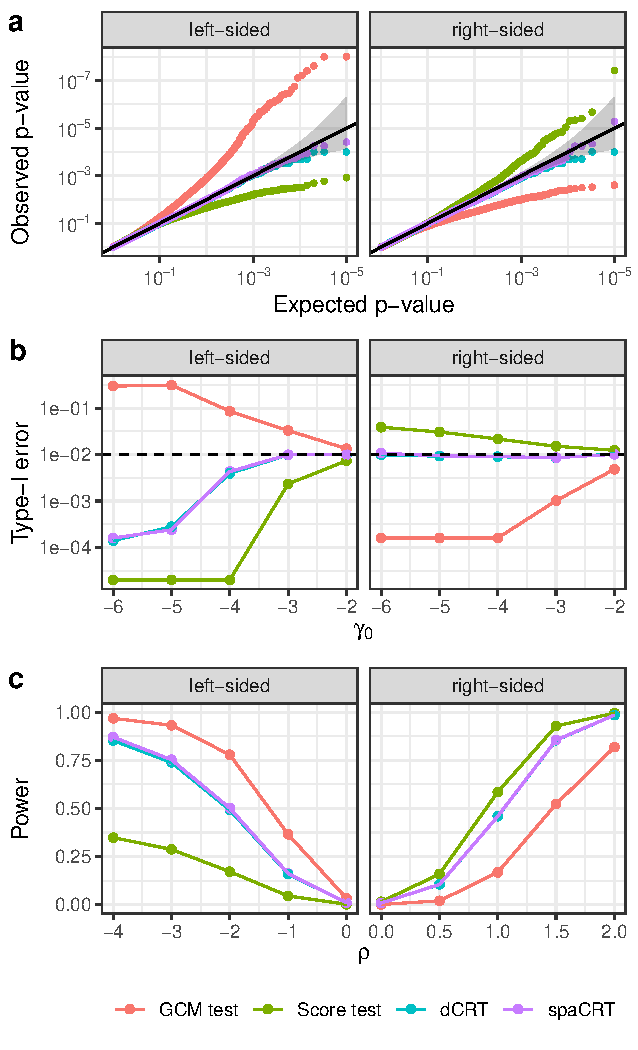
\includegraphics{figures-and-tables/simulation-summary.pdf}
	\caption{Summary of numerical simulation results for size parameter $r = 0.05$. (a) QQ-plots of the $p$-values obtained under the null hypothesis for $(\gamma_0, \beta_0) = (-3, -5)$. (b) Type-I error rates for $\beta_0 = -5$ as a function of the sparsity of $\srx$ ($\gamma_0$), when testing at level $\alpha = 0.01$. (c) Power for $(\gamma_0, \beta_0) = (-3, -5)$ as a function of the signal strength ($\rho$), when testing at level $\alpha = 0.01$.}
	\label{fig:simulation-summary}
\end{figure*}

Moreover, Figure~\ref{fig:simulation-computing-times} displays the computing times for the different methods in the settings considered in Figure~\ref{fig:simulation-summary}. We see that the spaCRT and GCM test are roughly tied for fastest, the score test is roughly half an order of magnitude slower than these two, while the dCRT is more than an order of magnitude slower. {\color{red} Finally, scatter plots in Figure~\ref{fig:simulation-dot-plot-varying-gamma-theta-0.05} confirm the alignment between $p$-values obtained from $\dCRT$ and $\spacrt$, which backs up the theoretical results proved in section \ref{sec:theory}. We refer additional scatter plots and how these scatter plots are generated to section \ref{sec:additional_figure_simulation}.}


\begin{figure*}[h!]
	\centering
	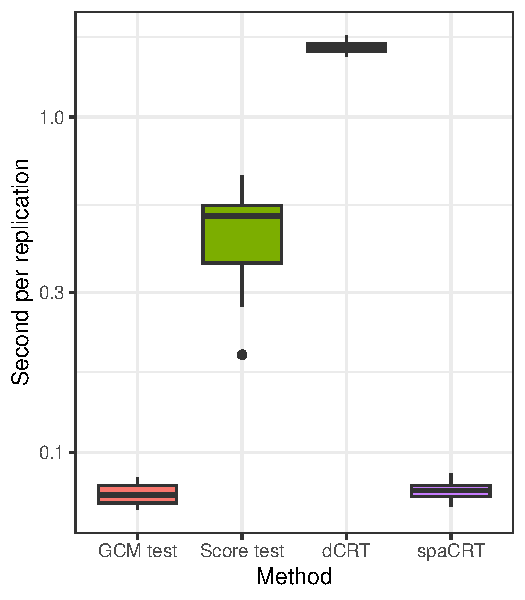
\includegraphics{figures-and-tables/simulation-computing-times.pdf}
	\caption{Computing times for numerical simulation with $r = 0.05$ and $\beta_0 = -5$.}
	\label{fig:simulation-computing-times}
\end{figure*}

\begin{figure*}
  \centering
  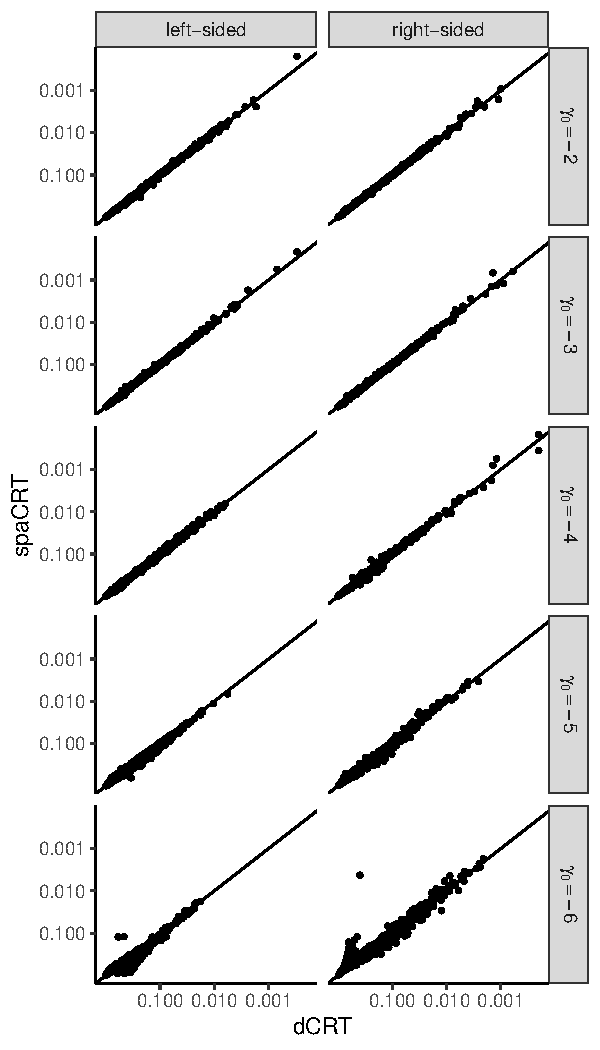
\includegraphics[width=0.8\textwidth]{figures-and-tables/simulation/QQ/plot-bin-NB-normal-B-50000-n-5000-5e3-n5-n5-disp-5e-2full-dCRT-spaCRT-varying-gamma.pdf}
  \caption{Scatter plots for the $p$-values of the left-sided and right-sided tests when varying $\gamma_0\in \{-6,-5,-4,-3,-2\}$ and fixing $\beta_0=-5$, with $\theta = 0.05$.}
  \label{fig:simulation-dot-plot-varying-gamma-theta-0.05}
\end{figure*}



\section{Real data analysis} \label{sec:real_data}

In this section, we compare the performance of the $\spacrt$ to those of alternative methods on the analysis of the \citet{Gasperini2019a} single-cell CRISPR screen dataset. 

\subsection{Overview of the data}

The Gasperini data contain expression measurements on 13,135 genes and CRISPR perturbations targeting 6,105 regulatory elements in $n =$ 207,324 cells. They also contain CRISPR perturbations intended as negative and positive controls. In particular, the data contain 51 non-targeting CRISPR perturbations, which do not target any regulatory element and therefore should have no effect on the expressions of any genes. Furthermore, the data contain 754 CRISPR perturbations targeting genes, rather than regulatory elements. These serve as positive controls, because they are known a priori to have effects on the expressions of the genes they target. Finally, the data contain measurements on six covariates, including four count-based covariates related to library size, one binary covariate indicating the experimental batch, and one continuous covariate indicating the proportion of reads mapping to mitochondrial genes in each cell.

\subsection{Analyses conducted}

\paragraph{Hypotheses tested.} In order to assess the Type-I error and power of the methods compared, we will use CRISPR perturbations intended as negative and positive controls, respectively. In particular, for Type-I error analysis, we test for association between each of the 51 negative control perturbations and each of 3,000 randomly sampled genes, for a total of 51 $\times$ 3,000 = 153,000 tests. We subsample the genes to reduce the computational burden of the analysis. To assess the power of each method, we test for association between each of the 754 positive control perturbations targeting genes and the gene they target, for a total of 754 tests. 

\paragraph{Methods compared.} We compare essentially the same methods as in the numerical simulations (recall Section~\ref{sec:simulation-setup}). The only difference is that we replace the dCRT with a faster variant implemented in the \verb|sceptre| package, in order to make the analysis computationally feasible. The \verb|sceptre| implementation of the dCRT fits a parametric curve to the resampling distribution of the test statistic based on a smaller number of resamples (a heuristic acceleration that is not theoretically justified). Furthermore, it is implemented in C++ for speed, unlike the other methods we consider, which are implemented in R. We apply left- and right-sided variants of each test on the negative control perturbation-gene pairs. For the positive control pairs, we apply only left-sided tests, since we are testing for a perturbation-induced decrease in gene expression.

\subsection{Results}

\paragraph{Type-I error.} Figure~\ref{fig:negative-control-qq-plots} displays QQ plots of the negative control $p$-values obtained from all four methods. The two tests relying on asymptotic normality, the GCM and score tests, exhibit severe $p$-value inflation for left- and right-sided tests, respectively. This finding is consistent with our simulation results (Figure~\ref{fig:simulation-summary}). On the other hand, the $\spacrt$ and \verb|sceptre| tests control Type-I error well for both left- and right-sided tests. {\color{red} We also report the number of false discoveries on the negative control pairs in Appendix~\ref{sec:additional_table_realdata}; the message from these results are consistent with that of the single testing results.}
\begin{figure*}[h!]
	\centering
	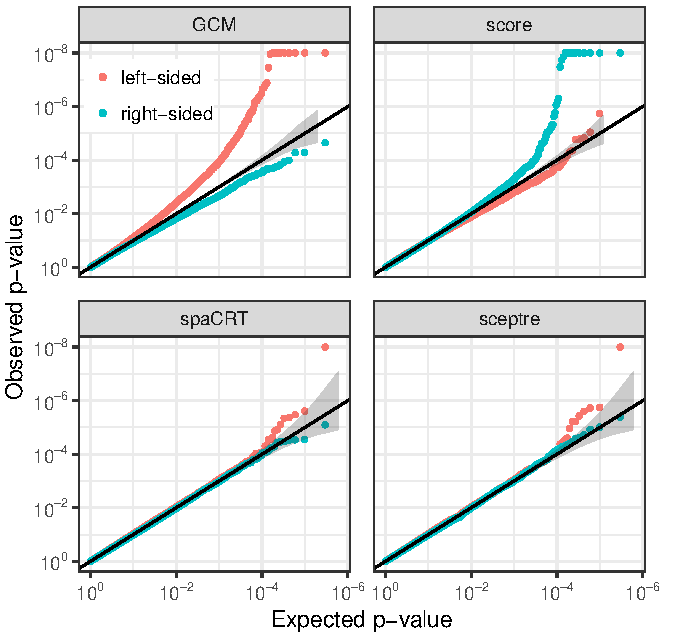
\includegraphics{figures-and-tables/condensed-without-stratification.pdf}
	\caption{Left- and right-sided $p$-values for negative control perturbation-gene pairs on the Gasperini data.}
	\label{fig:negative-control-qq-plots}
\end{figure*}

Next, we investigate the impact of the problem sparsity on calibration. Following \citep{Barry2024}, we measure sparsity in terms of the \textit{effective sample size} $\sum_{i = 1}^n \indicator(X_{i} Y_{i} > 0)$, which measures the number of cells with a given perturbation and nonzero expression of a given gene. Table~\ref{tab:sparsity_level_ess} displays the distribution of effective sample sizes across the negative control perturbation-gene pairs tested, showing that the effective samples sizes are vastly smaller than the number of cells, $n =$ 207,324. Furthermore, Figure~\ref{fig:qqplot_lowess} stratifies the QQ plots for each method by effective sample size, focusing on those pairs with effective sample size of at most 100. As expected based on our simulation study, we find more severe miscalibration for pairs with lower effective sample sizes, especially for the GCM and score tests, and to a lesser extent for \verb|sceptre| and the $\spacrt$. We carried out a similar analysis, stratifying the pairs based on the estimated size parameter (Figure~\ref{fig:qqplot_dispersion}). In line with our simulation results, we find that the GCM and score tests exhibit more miscalibration for smaller size parameters. 


\begin{table*}[h!]
  \centering
  \begin{tabular}[t]{lccccc}
  \toprule
    & Min. & 1st Qu. & Median & 3rd Qu. & Max.\\
  \midrule
  Effective sample size & 0   &   53   &  204  &   504  & 2044 \\
  \bottomrule
  \end{tabular}
  \caption{Effective sample size in subsampled dataset.}
  \label{tab:sparsity_level_ess}
\end{table*}

\paragraph{Power.}

Next, we compare the power of the four methods based on their left-sided $p$-values on the 754 positive control perturbation-gene pairs (Figure~\ref{fig:violinplot_scatter_power}). The signal is quite strong in these positive control pairs, as evidenced by small $p$-values for all four methods. \textcolor{red}{We remark that the $\spacrt$ overcomes the discreteness in the $p$-values returned by resampling-based methods such as the dCRT, delivering very small $p$-values in the presence of strong signals. Given the scale of the $p$-values, we refrain from making definitive conclusions about the relative power of the methods, but remark only that the $\spacrt$ appears at least as powerful as the alternative methods considered.}

\begin{figure*}[h!]
  \centering
  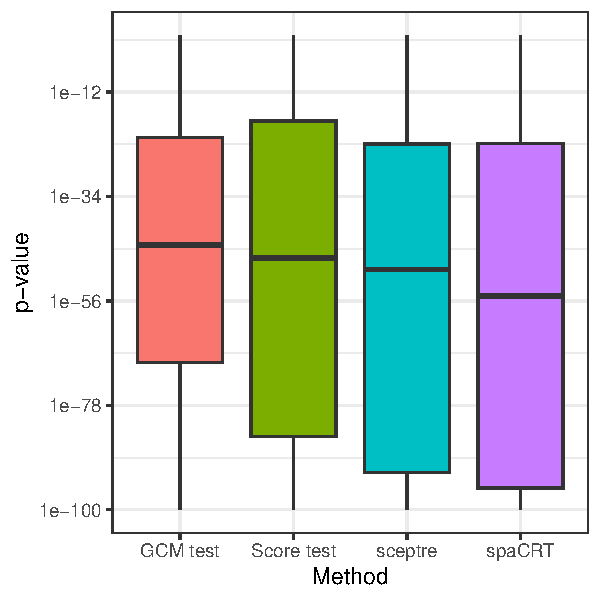
\includegraphics{figures-and-tables/power_boxplot.pdf}
\caption{Left-sided $p$-values computed on the 754 positive control perturbation-gene pairs in the \citet{Gasperini2019a} data.}
\label{fig:violinplot_scatter_power}
\end{figure*}

\paragraph{Computation.}

The excellent statistical properties of the $\spacrt$ do not come at the cost of computational efficiency. Since the \verb|sceptre| software is highly optimized, while the other methods are not, we benchmark our dCRT implementation (used in the numerical simulations) instead of \verb|sceptre|'s for computational efficiency. We use $M = $ 100,000 resamples for the dCRT, given the high multiplicity of the problem (recall Section~\ref{sec:statistical-computational-challenges}). To assess running time, we paired two randomly sampled genes with each of the 51 non-targeting perturbations, for a total of 102 perturbation-gene pairs. We find that the $\spacrt$ is roughly as fast as the GCM test, about five times faster than the score test, and about 250 times faster than the dCRT.

\begin{table}[!h]
\centering
\caption{\label{tab:time_comparison}Computation time per perturbation-gene pair on the Gasperini data. Times are reported in seconds.}
\centering
\begin{tabular}[t]{lrr}
\toprule
Method & Mean & Std dev\\
\midrule
GCM test & 4.0 & 1.9\\
dCRT & 1002.1 & 279.5\\
spaCRT & 4.0 & 1.9\\
Score test & 19.9 & 9.3\\
\bottomrule
\end{tabular}
\end{table}


\section{Discussion} \label{sec:discussion}

In this paper, we introduce the $\spacrt$, a new conditional independence test enjoying several desirable properties: (1) It is completely resampling-free, which makes it very computationally efficient. (2) It is asymptotically equivalent to the doubly robust dCRT, so it has Type-I error control without requiring the model-X assumption. (3) It has excellent Type-I error control and power in both numerical simulations and real data analysis. The $\spacrt$ is particularly well-suited to single-cell CRISPR screen data analysis, where it can significantly accelerate the state-of-the-art \verb|sceptre| software without sacrificing statistical performance.

Despite the attractive properties of the $\spacrt$, the current work still has several limitations. First, there remains a gap between our theoretical guarantees and the practical performance of the $\spacrt$ and $\dCRT$. We have shown that both of these tests have Type-I error control asymptotically, but we have not theoretically justified why these tests perform so well in finite samples, compared with asymptotic tests like the GCM and score tests. Second, we have focused on approximating the $\dCRT$ in this paper, but the conditional randomization test framework is applicable to general test statistics. It would be interesting to see how the saddlepoint approximation can be extended to other test statistics.

\section{Acknowledgments}

We acknowledge the Wharton research computing team for their help with our use of the Wharton high-performance computing cluster for the numerical simulations and real data analyses in this paper. This work was partially support by NSF DMS-2113072 and NSF DMS-2310654.




\clearpage 

\printbibliography

\clearpage

\appendix

\section{Probability theory preliminaries}

\subsection{Single probability space embedding}
To better state and understand the conditional convergence result, the following lemma helps to embed all the random variables into one big probability space.

\begin{lemma}[Embedding into a single probability space, Lemma 14 in \cite{Niu2022a}]\label{lem:embedding}
	Consider a sequence of probability spaces $\{(\P_n,\Omega_n,\mathcal{G}_n),n \geq 1\}$. For each $n$, let $\{W_{i,n}\}_{i \geq 1}$ be a collection of integrable random variables defined on $(\P_n,\Omega_n,\mathcal{G}_n)$ and let $\mathcal F_n \subseteq \mathcal G_n$ be a $\sigma$-algebra. Then there exists a single probability space $(\widetilde{\P}, \widetilde{\Omega}, \widetilde{\mathcal G})$, random variables $\{\widetilde W_{i,n}\}_{i,n \geq 1}$ on $(\widetilde{\P}, \widetilde{\Omega}, \widetilde{\mathcal G})$, and $\sigma$-fields $\widetilde{\mathcal F}_n \subseteq \widetilde{\mathcal G}$ for $n \geq 1$, such that for each $n$, the joint distribution of $(\{W_{i,n}\}_{i \geq 1}, \{\E[W_{i,n}\mid\mathcal F_n]\}_{i \geq 1})$ on $(\P_n,\Omega_n,\mathcal{G}_n)$ coincides with that of $(\{\widetilde W_{i,n}\}_{i \geq 1}, \{\E[\widetilde W_{i,n}\mid \widetilde{\mathcal F}_n]\}_{i \geq 1})$ on $(\widetilde{\P}, \widetilde{\Omega}, \widetilde{\mathcal G})$.
\end{lemma}
\noindent With the above Lemma, we are safe to state any almost sure statement which can be interpreted within one probability space. 

\subsection{Some facts about natural exponential family}

Consider the NEF with probability density function
\begin{align*}
  f(x|\theta)=h(x)\exp(\theta x-A(\theta)).
\end{align*}
Then there is one-to-one correspondence between the moments of the random variable from NEF and the derivative of the log-partition function $A(\theta)$. We summarise the relationship in the following Lemma.

\begin{lemma}[Chapter 1.2 in \cite{Efron2022}]\label{lem:moment_logpartition}
  Suppose $X\sim f(x|\theta)$ then the following identities hold:
  \begin{enumerate}
    \item $\E[X]=A'(\theta)$;
    \item $\E[X^2]-(\E[X])^2=A''(\theta)$;
    \item $\E[(X-\E[X])^3]=A^{(3)}(\theta)$;
    \item $\E[(X-\E[X])^4]-3\left(\E[(X-\E[X])^2]\right)^2=A^{(4)}(\theta)$.
  \end{enumerate}
\end{lemma}


\section{Preliminaries for saddlepoint approximation}\label{sec:saddlepoint_prelim}

Let $W$ be a random variable on $(\Omega, \mathcal F, \P)$ and let $\mathcal G \subseteq \mathcal F$ be a $\sigma$-algebra. Consider the following definitions.

\begin{definition}[CSE distribution]\label{def:cse_distribution}
Consider a random variable $\theta \in \mathcal G$ such that $\theta \geq 0$ almost surely and a constant $\beta > 0$. We say $W|\mathcal{G}$ is \textit{conditionally sub-exponential} (CSE) with parameters $(\theta, \beta)$ if, almost surely,
\begin{align*}
\P\left[|W|\geq t \mid \mathcal{G}\right]\leq \theta\exp(-\beta t),\ \text{for all } t>0.
\end{align*}
We denote this property via $W|\mathcal G \sim \text{CSE}(\theta, \beta)$.
\end{definition}

\begin{definition}[CCS distribution]\label{def:ccs_distribution}
	Consider a random variable $\nu \in \mathcal G$ such that $\nu \geq 0$ almost surely. We say $W|\mathcal{G}$ is \textit{conditionally compactly supported} (CCS) on $[-\nu, \nu]$ if
\begin{align*}
W \in [-\nu,\nu] \quad \text{almost surely}.
\end{align*}
We denote this property via $W|\mathcal G \sim \text{CCS}(\nu)$.
\end{definition}

Consider a triangular array $\{W_{in}\}_{1 \leq i \leq n, n \geq 1}$ and $\sigma$-algebra $\mathcal{F}_n$, so that $\E[W_{in}|\mathcal{F}_n] = 0$ for each $(i, n)$, and $\{W_{in}\}_{1 \leq i \leq n}$ are independent conditionally on $\mathcal{F}_n$ for each $n$. Now, we impose assumptions on the triangular array $\{W_{in}\}_{1 \leq i \leq n, n \geq 1}$ in terms of Definition \ref{def:cse_distribution}-\ref{def:ccs_distribution}. We assume throughout this section that Assumption~\ref{assu:cse} or Assumption~\ref{assu:ccs} holds.
\begin{assumption}[CSE condition]\label{assu:cse}
There exist $\theta_n \in \mathcal F_n$ and $\beta > 0$ such that 
\begin{equation}\label{eq:cse_condition}
W_{in}|\mathcal F_n \sim \textnormal{CSE}(\theta_n, \beta) \text{ for all } i, n, \quad \theta_n < \infty \text{ almost surely}, \quad \theta_n = O_{\P}(1).
\end{equation}
\end{assumption}
\begin{assumption}[CCS condition]\label{assu:ccs}
There exist $\nu_{in} \in \mathcal F_n$ such that 
\begin{align}\label{eq:ccs_condition}
W_{in}|\mathcal F_n \sim \textnormal{CCS}(\nu_{in}), \quad \nu_{in}<\infty\ \text{almost surely}, \quad \text{and} \quad \frac{1}{n}\sum_{i=1}^n \nu_{in}^4=O_{\P}(1).
\end{align}
\end{assumption}

Given the sequence $x_n\in\mathcal{F}_n$, we would like to approximate tail probabilities for the average $W_n\equiv \frac{1}{n}\sum_{i=1}^n W_{in}$:
\begin{equation*}
	\P[W_n\geq x_n|\mathcal{F}_n]
\end{equation*}
We will approximate this tail probability via the saddlepoint approximation. This requires the existence of the conditional cumulant generating function (CGF):
\begin{equation*}
  K_n(s|\mathcal{F}_n) \equiv \frac{1}{n}\sum_{i=1}^n K_{in}(s|\mathcal{F}_n),\ K_{in}(s|\mathcal{F}_n)\equiv \log \E[\exp(sW_{in})|\mathcal{F}_n].
\end{equation*}
Here $K_{in}(\cdot\mid\mathcal{F}_n)$ is the conditional CGF of $W_{in}$. The very first step in saddlepoint approximation is to find the tilting parameter $\hat s_n$ solving the \textit{saddlepoint equation}
\begin{equation}\label{eq:saddlepoint-equation}
	K_n'(s|\mathcal{F}_n)=x_n.
\end{equation}
Then the validity of the saddlepoint approximation is formalized in the following two lemmas.

\begin{lemma}[Lemma 1 in \cite{Niu2024}]\label{lem:finite_cgf}
  Suppose Assumption~\ref{assu:cse} or Assumption~\ref{assu:ccs} holds. Then, there exists a probability-one event $\mathcal A$ and an $\varepsilon > 0$ such that, on $\mathcal A$,
  \begin{align}
  K_{in}(s) < \infty\quad \text{for any } s\in (-\varepsilon,\varepsilon)\ \text{and}\ \text{for all}\ i \leq n,\ n \geq 1 \label{eq:finite_cgf}.
  \end{align}
  In particular, when Assumption \ref{assu:cse} holds, $\varepsilon=\beta/8$ and when Assumption \ref{assu:ccs} holds, $\varepsilon=1/8$.
  \end{lemma}



\begin{lemma}[Theorem 1 in \cite{Niu2024}]\label{cor:spa_conditional_inid}
	Let $W_{in}$ be a triangular array of random variables that are mean-zero and independent for each $n$, conditionally on $\mathcal F_n$. Suppose either Assumption \ref{assu:cse} or Assumption \ref{assu:ccs} holds, and that
	\begin{align}\label{eq:lower_bound_conditional_variance}
		\frac{1}{n}\sum_{i=1}^n \E[W_{in}^2 \mid \mathcal{F}_n]=\Omega_{\P}(1).
	\end{align}
	Let $x_n \in \mathcal F_n$ be a sequence with $x_n \overset{\P} \rightarrow 0$ and $\varepsilon>0$ is defined as in Lemma \ref{lem:finite_cgf}. Then, the saddlepoint equation~\eqref{eq:saddlepoint-equation} has a unique and finite solution $\hat s_n \in [-\varepsilon/2, \varepsilon/2]$ with probability approaching 1 as $n \rightarrow \infty$. If we define $\lambda_n \equiv \hat s_n\sqrt{nK_n''(\hat s_n\mid\mathcal{F}_n)}$ and
	  \begin{align*}
		r_n \equiv
		\begin{cases}
		  \sgn(\hat s_n) \sqrt{2n( \hat s_n x_n - K_n(\hat s_n\mid\mathcal{F}_n))} & \text{if } \hat s_n x_n - K_n(\hat s_n\mid\mathcal{F}_n)\geq 0;\\
		  \mathrm{sgn}(\hat s_n) & \text{otherwise},
		\end{cases}
		\end{align*}
	  then
	  \begin{align*}
		\P\left[\left.\frac{1}{n}\sum_{i = 1}^n W_{in} \geq x_n\ \right|\ \mathcal{F}_n\right]=\left(1-\Phi(r_n)+\phi(r_n)\left\{\frac{1}{\lambda_n}-\frac{1}{r_n}\right\}\right)(1+o_{\P}(1)).
	  \end{align*}
    and 
    \begin{align*}
      \P\left[1-\Phi(r_n)+\phi(r_n)\left\{\frac{1}{\lambda_n}-\frac{1}{r_n}\right\}>0\right]\rightarrow1 \text{ as }n\rightarrow\infty.
    \end{align*}
  \end{lemma}



\section{Some useful lemmas and proofs}\label{sec:useful_lemma}


\begin{lemma}[Lemma 3 in \cite{Niu2022a}]\label{lem:unified_asymptotic_equivalence}
	Consider two hypothesis tests based on the same test statistic $T_n(\srx, \sry, \srz)$ but different critical values:
	\begin{equation*}
		\phi_n^1(\srx, \sry, \srz) \equiv \indicator(T_n(\srx, \sry, \srz) > C_n(\srx, \sry, \srz)); \quad \phi_n^2(\srx, \sry, \srz) \equiv \indicator(T_n(\srx, \sry, \srz) > z_{1-\alpha}). 
	\end{equation*}
	If the critical value of the first converges in probability to that of the second:
	\begin{equation*}
		C_n(\srx, \sry, \srz) \convp z_{1-\alpha}
	\end{equation*}
	and the test statistic does not accumulate near the limiting critical value:
	\begin{equation}
		\lim_{\delta \rightarrow 0}\limsup_{n \rightarrow \infty}\ \P_{\law_n}[|T_n(\srx, \sry, \srz)-z_{1-\alpha}| \leq \delta] = 0,
		\label{eq:non-accumulation-app}
	\end{equation}
	then the two tests are asymptotically equivalent:
	\begin{equation*}
		\lim_{n \rightarrow \infty}\P_{\law_n}[\phi_n^{1}(\srx, \sry, \srz) = \phi_n^2(\srx, \sry, \srz)] = 1.
	\end{equation*}
\end{lemma}


\paragraph{\textbf{Regularity condition:}}
there exists $\delta>0$ such that for a sequence of laws $\law_n$ and its estimate $\lawhat_n$, the following assumptions hold:
\begin{align}
    (\widehat{S}_n^{\dCRT})^2\equiv\frac{1}{n}\sum_{i=1}^n\V_{\lawhat_n}[\srx_{in}\mid \srz_{in}](\sry_{in}-\widehat{\mu}_{n,y}(\srz_{in}))^2=\Omega_\P(1) \label{eq:variance_lower_bound};\\
    \frac{1}{n^{1+\delta/2}} \sum_{i=1}^n |\sry_{in}-\widehat \mu_{n,y}(\srz_{in})|^{2+\delta}\E_{\lawhat_n}[|\srxk_{in}-\widehat\mu_{n,x}(\srz_{in})|^{2+\delta}\mid \srx,\srz] =o_\P(1)\label{eq:Lyapunov_condition_2};\\
    \V_{\lawhat_n}[\srx_{in}|\srz_{in}],(\sry_{in}-\widehat{\mu}_{n,y}(\srz_{in}))^2,(\sry_{in}-\mu_{n,y}(\srz_{in}))^2<\infty\ \text{almost surely}\label{eq:non_degeneracy}.
\end{align}

\begin{lemma}[Theorem 9 in \cite{Niu2022a}]\label{lem:quantile_convergence_ptwise}
	Let $\law_n$ be a sequence of laws and $\lawhat_n$ be a sequence of estimates. Suppose  there exists a sequence of laws $\law_n$ satisfying all the assumptions in \textbf{Regularity condition}. Then, the quantile of 
  \begin{align}\label{eq:normalized_dcrt_stats}
    T_n^{\ndCRThat}(\srxk,\srx,\sry,\srz)\equiv \frac{T_n^{\dCRT}(\srxk,\srx,\sry,\srz)}{\widehat S_n^{\dCRT}}
  \end{align}
  converges to the quantile of the standard normal distribution pointwisely in probability, i.e., for any $p\in(0,1)$,
	\begin{align*}
		\Q_{p}\left[n^{1/2}T_n^{\ndCRThat}(\srxk,\srx,\sry,\srz)|\srx,\sry,\srz\right]\convp z_{p}.
	\end{align*}
\end{lemma}

\begin{lemma}[Corollary 6 in \cite{Niu2022a}]\label{lem:wlln}
  Let $X_{in}$ be a triangular array of random variables, such that $X_{in}$ are independent for each $n$. If for some $\delta>0$ we have 
  \begin{align}\label{eq:moment_condition_wlln}
    \frac{1}{n^{1+\delta}}\sum_{i=1}^n \E[|X_{in}|^{1+\delta}]\rightarrow 0,
  \end{align}
  then 
  \begin{align*}
    \frac{1}{n}\sum_{i=1}^n (X_{in}-\E[X_{in}])\overset{\P}{\rightarrow}0.
  \end{align*}
  The condition \eqref{eq:moment_condition_wlln} is satisfied when 
  \begin{align*}
    \sup_{1\leq i\leq n}\E[|X_{in}|^{1+\delta}]=o(n^\delta).
  \end{align*}
\end{lemma}

\begin{lemma}[Dominance of higher moment]\label{lem:moment_dominance}
  For any $1<p<q<\infty$, the following inequality is true almost surely:
  \begin{align*}
    \frac{1}{n}\sum_{i=1}^n \E[|X_{in}|^{p}|\mathcal{F}_n]\leq \left(\frac{1}{n}\sum_{i=1}^n \E[|X_{in}|^{q}|\mathcal{F}_n]\right)^{p/q}.
  \end{align*}
\end{lemma}


\begin{lemma}[Conditional H\"older inequality, \cite{Swanson2019}, Theorem 6.60]\label{lem:cond_holder}
	Let $W_1$ and $W_2$ be random variables and let $\mathcal F$ be a $\sigma$-algebra. If for some $q_1, q_2 \in (1,\infty)$ with $\frac{1}{q_1} + \frac{1}{q_2} = 1$ we have $\E[|W_1|^{q_1}], \E[|W_2|^{q_2}] < \infty$, then
	\begin{align*}
		\E[|W_1 W_2| \mid \mathcal F] \leq (\E[|W_1|^{q_1} \mid \mathcal F])^{1/q_1}(\E[|W_2|^{q_2} \mid \mathcal F])^{1/q_2} \quad \text{almost surely}.
	\end{align*}
\end{lemma}

\begin{lemma}[Conditional Jensen inequality, \cite{Davidson2003}, Theorem 10.18] \label{lem:conditional-jensen}
	Let $W$ be a random variable and let $\phi$ be a convex function, such that $W$ and $\phi(W)$ are integrable. For any $\sigma$-algebra $\mathcal F$, we have the inequality
	\begin{equation*}
		\phi(\E[W \mid \mathcal F]) \leq  \E[\phi(W) \mid \mathcal F] \quad \text{almost surely}.
	\end{equation*}
\end{lemma}

\subsection{Proof of Lemma \ref{lem:moment_dominance}}

\begin{proof}[Proof of Lemma \ref{lem:moment_dominance}]
  By Lemma \ref{lem:cond_holder}, we have
  \begin{align*}
    \frac{1}{n}\sum_{i=1}^n \E[|X_{in}|^{p}|\mathcal{F}_n]
    &
    \leq 
    \frac{1}{n}\left(\sum_{i=1}^n \left(\E[|X_{in}|^{p}|\mathcal{F}_n]\right)^{q/p}\right)^{p/q}n^{1-p/q}\\
    &
    =\left(\frac{1}{n}\sum_{i=1}^n \left(\E[|X_{in}|^{p}|\mathcal{F}_n]\right)^{q/p}\right)^{p/q}.
  \end{align*}
  We use Jensen's inequality, Lemma \ref{lem:conditional-jensen}, to obtain
  \begin{align*}
    \frac{1}{n}\sum_{i=1}^n \E[|X_{in}|^{p}|\mathcal{F}_n]\leq \left(\frac{1}{n}\sum_{i=1}^n \E[|X_{in}|^{q}|\mathcal{F}_n]\right)^{p/q}.
  \end{align*}
\end{proof}





\section{Proof of results in section \ref{sec:theory}}


\subsection{Proof of Theorem \ref{thm:validity_spacrt}}

We have conditional CGF 
\begin{equation}
K_{in}(s|\mathcal{F}_n) = A(\widehat \theta_{n,x}(\srz_{in})+a_{in}s)-A(\widehat \theta_{n,x}(\srz_{in}))-a_{in}sA'(\widehat \theta_{n,x}(\srz_{in})).
\end{equation}
We will apply Lemma \ref{cor:spa_conditional_inid} and thus verify the conditions in the lemma. We first verify the variance condition \eqref{eq:lower_bound_conditional_variance}.

\paragraph{\textbf{Verification of \eqref{eq:lower_bound_conditional_variance}}:}
Compute $K_{in}''(s\mid \mathcal{F}_n)= a_{in}^2A''(\widehat \theta_{n,x}(\srz_{in})+a_{in}s)$. Then it suffices to guarantee 
\begin{align*}
  \frac{1}{n}\sum_{i=1}^n \E[W_{in}^2|\mathcal{F}_n]=\frac{1}{n}\sum_{i=1}^n K_{in}''(0\mid \mathcal{F}_n)=\frac{1}{n}\sum_{i=1}^n a_{in}^2A''(\widehat \theta_{n,x}(\srz_{in}))=\Omega_\P(1).
\end{align*}

\noindent Next we verify assumption \ref{assu:cse} and condition \eqref{eq:ccs_assumption} respectively.

\paragraph{Verification of Assumption \ref{assu:cse} with condition \eqref{eq:cse_assumption} and \eqref{eq:upper_bound_theta_a}:} 

We denote the conditional upper tail probability and lower probability respectively as 
\begin{align*}
  L_{X,\mathcal{F}_n}(a)\equiv \P\left[X\leq a|\mathcal{F}_n\right],\ U_{X,\mathcal{F}_n}(a)\equiv \P\left[X\geq a|\mathcal{F}_n\right].
\end{align*}
Then by the definition of CSE distribution (Definition \ref{def:cse_distribution}),  we can compute 
\begin{align*}
  &
  \P[W_{in}\geq t|\mathcal{F}_n]\\
  &
  =\P[a_{in}(\srxk_{in}-A'(\widehat \theta_{n,x}(\srz_{in})))\geq t|\mathcal{F}_n]\\
  &
  =\indicator(a_{in}>0)U_{\srxk_{in},\mathcal{F}_n}\left(\frac{t}{a_{in}}+A'(\widehat{\theta}_{n,x}(\srz_{in}))\right)+\indicator(a_{in}<0)L_{\srxk_{in},\mathcal{F}_n}\left(\frac{t}{a_{in}}+A'(\widehat{\theta}_{n,x}(\srz_{in}))\right)
\end{align*}
Then by the definition of natural exponential family, we can write 
\begin{align*}
  &
  \indicator(a_{in}>0)U_{\srxk_{in},\mathcal{F}_n}\left(\frac{t}{a_{in}}+A'(\widehat{\theta}_{n,x}(\srz_{in}))\right)\\
  &
  =\indicator(a_{in}>0)\int_{t/a_{in}+A'(\widehat{\theta}_{n,x}(\srz_{in}))}^{\infty}\exp(\widehat{\theta}_{n,x}(\srz_{in})x-A(\widehat{\theta}_{n,x}(\srz_{in})))h(x)dx\\
  &
  =\indicator(a_{in}>0)\int_{t/a_{in}+A'(\widehat{\theta}_{n,x}(\srz_{in}))}^{\infty}\exp(\widehat{\theta}_{n,x}(\srz_{in})x+a_{in}x -a_{in}x-A(\widehat{\theta}_{n,x}(\srz_{in})))h(x)dx\\
  &
  \leq \indicator(a_{in}>0)\int_{t/a_{in}+A'(\widehat{\theta}_{n,x}(\srz_{in}))}^{\infty}\exp((\widehat{\theta}_{n,x}(\srz_{in})+a_{in})x-A(\widehat{\theta}_{n,x}(\srz_{in})))h(x)\mathrm{d}x\\
  &
  \qquad\times \exp(-t-a_{in}A'(\widehat{\theta}_{n,x}(\srz_{in})))\\
  &
  \leq \indicator(a_{in}>0)\int_{t/a_{in}+A'(\widehat{\theta}_{n,x}(\srz_{in}))}^{\infty}\exp((\widehat{\theta}_{n,x}(\srz_{in})+a_{in})x-A(a_{in}+\widehat{\theta}_{n,x}(\srz_{in})))h(x)\mathrm{d}x\\
  &
  \qquad\times \exp(A(a_{in}+\widehat{\theta}_{n,x}(\srz_{in}))-A(\widehat{\theta}_{n,x}(\srz_{in})))\exp(-t-a_{in}A'(\widehat{\theta}_{n,x}(\srz_{in})))\\
  &
  \leq \indicator(a_{in}>0)\exp(A(\widehat{\theta}_{n,x}(\srz_{in})+a_{in})-A(\widehat{\theta}_{n,x}(\srz_{in}))-a_{in}A'(\widehat{\theta}_{n,x}(\srz_{in})))\exp(-t)\\
  &
  \leq \indicator(a_{in}>0)\exp(|A(\widehat{\theta}_{n,x}(\srz_{in})+a_{in})|+|A(\widehat{\theta}_{n,x}(\srz_{in}))|+|a_{in}||A'(\widehat{\theta}_{n,x}(\srz_{in}))|)\exp(-t)
\end{align*}
Similarly, we can derive the upper bound for the lower tail Probability: 
\begin{align*}
  &
  \indicator(a_{in}<0)L_{\srxk_{in},\mathcal{F}_n}\left(\frac{t}{a_{in}}+A'(\widehat{\theta}_{n,x}(\srz_{in}))\right)\\
  &
  =\indicator(a_{in}<0)\int_{-\infty}^{t/a_{in}+A'(\widehat{\theta}_{n,x}(\srz_{in}))}\exp(\widehat{\theta}_{n,x}(\srz_{in})x-A(\widehat{\theta}_{n,x}(\srz_{in})))h(x)dx\\
  &
  =\indicator(a_{in}<0)\int_{-\infty}^{t/a_{in}+A'(\widehat{\theta}_{n,x}(\srz_{in}))}\exp(\widehat{\theta}_{n,x}(\srz_{in})x+a_{in}x - a_{in}x-A(\widehat{\theta}_{n,x}(\srz_{in})))h(x)dx\\
  &
  \leq \indicator(a_{in}<0)\exp(A(\widehat{\theta}_{n,x}(\srz_{in})+a_{in})-A(\widehat{\theta}_{n,x}(\srz_{in}))-a_{in}A'(\widehat{\theta}_{n,x}(\srz_{in})))\exp(-t)\\
  &
  \leq \indicator(a_{in}<0)\exp(|A(\widehat{\theta}_{n,x}(\srz_{in})+a_{in})|+|A(\widehat{\theta}_{n,x}(\srz_{in}))|+|a_{in}||A'(\widehat{\theta}_{n,x}(\srz_{in}))|)\exp(-t).
\end{align*}
Then we have for any $t>0$,
\begin{align*}
  &
  \P[W_{in}\geq t|\mathcal{F}_n]\\
  &
  \leq \exp(|A(\widehat{\theta}_{n,x}(\srz_{in})+a_{in})|+|A(\widehat{\theta}_{n,x}(\srz_{in}))|+|a_{in}||A'(\widehat{\theta}_{n,x}(\srz_{in}))|)\exp(-t)\\
  &
  \leq \exp(\sup_{i}|A(\widehat{\theta}_{n,x}(\srz_{in})+a_{in})|+\sup_{i}|A(\widehat{\theta}_{n,x}(\srz_{in}))|+\sup_i|a_{in}||A'(\widehat{\theta}_{n,x}(\srz_{in}))|)\exp(-t).
\end{align*}
Choosing
\begin{align*}
  \theta_n=\exp\left(\sup_{i}|A(\widehat{\theta}_{n,x}(\srz_{in})+a_{in})|+\sup_{i}|A(\widehat{\theta}_{n,x}(\srz_{in}))|+\sup_i|a_{in}||A'(\widehat{\theta}_{n,x}(\srz_{in}))|\right)
\end{align*}
and $\beta = 1$, we need to verify 
\begin{align*}
  \theta_n=O_{\P}(1)\text{ and }\theta_n<\infty,\text{ almost surely}.
\end{align*}
Since by condition \eqref{eq:upper_bound_theta_a}, we know $\sup_i|a_{in}|\leq \sup_i |\sry_{in}|+\sup_{i}|\widehat{\mu}_{n,y}(\srz_{in})|<\infty $ almost surely and $|\widehat{\theta}_{n,x}(\srz_{in})|<\infty$ almost surely, we know $\theta_n<\infty$ almost surely. Now we prove $\theta_n=O_{\P}(1)$. By condition \eqref{eq:cse_assumption}, we know for any fixed $\delta>0$, there exists $M(\delta)>0$ such that 
\begin{align*}
  \P\left[\mathcal{S}\right]\geq 1-\delta,\text{ where }\mathcal{S}\equiv\left\{\sup_{i}|\widehat{\theta}_{n,x}(\srz_{in})|,\ \sup_{i}|a_{in}|\in [0,M(\delta)]\right\}.
\end{align*}
Then on the event $\mathcal{S}$, we know 
\begin{align*}
  \sup_{i}|A(\widehat{\theta}_{n,x}(\srz_{in})+a_{in})|\leq \sup_{x\in [-2M(\delta),2M(\delta)]}|A(x)|
\end{align*}
and 
\begin{align*}
  \sup_{i}|A'(\widehat{\theta}_{n,x}(\srz_{in}))|\leq \sup_{x\in [-M(\delta),M(\delta)]}|A'(x)|.
\end{align*}
Similarly, on the event $\mathcal{S}$, we have 
\begin{align*}
  \sup_{i}|a_{in}|\leq M(\delta),\ \sup_{i}|A(\widehat{\theta}_{n,x}(\srz_{in}))|\leq \sup_{x\in [-2M(\delta),2M(\delta)]}|A(x)|.
\end{align*}
Therefore we have 
\begin{align*}
  \P\left[\theta_n\leq \exp\left(2\sup_{x\in [-2M(\delta),2M(\delta)]}|A(x)|+M(\delta)\sup_{x\in [-M(\delta),M(\delta)]}|A'(x)|\right)\right]\geq\P[\mathcal{S}]\geq 1-\delta.
\end{align*}
Therefore we have $\theta_n=O_{\P}(1)$. Thus $\varepsilon=\beta/8=1/8$ according to Lemma \ref{lem:finite_cgf}.

\paragraph{Verification of Assumption \ref{assu:ccs} with condition \eqref{eq:upper_bound_theta_a} and \eqref{eq:ccs_assumption}:}

By condition \eqref{eq:ccs_assumption}, we know 
\begin{align*}
  \indicator(\widetilde{X}_{in}\in [-S,S])=1,\text{ almost surely}.
\end{align*}
This implies that for any $F\in\mathcal{F}_n$, we have 
\begin{align*}
  \int_F \indicator\left(\widetilde{X}_{in}\in [-S,S]\right)d\mathbb{P}=\int_F 1 \mathrm{d}\mathbb P.
\end{align*}
Thus we know 
\begin{align*}
  \P[\widetilde{X}_{in}\in [-S,S]|\mathcal{F}_n]=\E[\indicator(\widetilde{X}_{in}\in [-S,S])|\mathcal{F}_n]=1,\text{ almost surely}.
\end{align*}
Thus we have
\begin{align*}
  \P\left[a_{in}(\srxk_{in}-\widehat{\mu}_{n,x}(\srz_{in}))\in [-2|a_{in}|S,2|a_{in}|S]|\mathcal{F}_n\right]=1,\text{ almost surely}.
\end{align*}
Then again by condition \eqref{eq:upper_bound_theta_a}, we know 
\begin{align*}
  |a_{in}|\leq |\sry_{in}|+|\widehat{\mu}_{n,x}(\srz_{in})|<\infty,\text{ almost surely}.
\end{align*}
Moreover, by condition \eqref{eq:ccs_assumption}, we know 
\begin{align*}
  \frac{1}{n}\sum_{i=1}^n 16S^4a_{in}^4=\frac{16S^4}{n}\sum_{i=1}^n (\sry_{in}-\widehat{\mu}_{n,y}(\srz_{in}))^4=O_{\P}(1).
\end{align*}
Choosing $\nu_{in}=2|a_{in}|S$, we complete the proof for CCS distribution. Thus $\varepsilon=1/8$ according to Lemma \ref{lem:finite_cgf}.


  \subsection{Proof of Theorem \ref{thm:asymptotic_equivalence}}

  \begin{proof}[Proof of Theorem \ref{thm:asymptotic_equivalence}]
	Define the auxiliary test 
	  \begin{align*}
		  \phi^{\aux}_{n,\alpha}\equiv \indicator\left(\frac{n^{1/2}T_n^{\dCRT}(\srx,\sry,\srz)}{\widehat{S}_n^{\dCRT}}>\Q_{1-\alpha(1+M_n)}\left[n^{1/2}T_n^{\ndCRThat}(\widetilde{X},X,Y,Z)|X,Y,Z\right]\right)
	  \end{align*}
	where $T_n^{\ndCRThat}(\srxk,\srx,\sry,\srz)$ is defined in \eqref{eq:normalized_dcrt_stats} and $M_n$ is the sequence such that
	\begin{align*}
	  \P\left(T_n^{\dCRT}(\srxk,\srx,\sry,\srz)\geq T_n^{\dCRT}(\srx,\sry,\srz)|\mathcal{F}_n\right)=p_{\spacrt}(1+M_n),\text{ almost surely}.
	\end{align*}
	  Notice the tests $\phi_{n,\alpha}^{\spacrt}$ and $\phi_{n,\alpha}^{\aux}$ are equivalent as long as $M_n \in (-1, 1/\alpha - 1)$. Indeed, we have 
	\begin{align*}
	  \P[\phi_{n,\alpha}^{\spacrt}\neq \phi_{n,\alpha}^{\aux}]\leq \P[\widehat S_n^{\dCRT}=0]+\P[M_n \notin (-1, 1/\alpha - 1)]\rightarrow0
	\end{align*}
	due to assumption \eqref{eq:variance_lower_bound} and that $M_n=o_{\P}(1)$. Thus we only need to verify $\phi_{n,\alpha}^{\aux}$ and $\phi_{n,\alpha}^{\dCRT}$ are asymptotically equivalent. To this end, we consider another test 
	  \begin{align*}
		  \phi_{n,\alpha}^{\asy}\equiv \indicator\left(\frac{n^{1/2}T_n^{\dCRT}(\srx,\sry,\srz)}{\widehat{S}_n^{\dCRT}}>z_{1-\alpha}\right).
	  \end{align*}
	We will prove $\phi_{n,\alpha}^{\aux},\phi_{n,\alpha}^{\asy}$ are asymptotically equivalent and $\phi_{n,\alpha}^{\dCRT},\phi_{n,\alpha}^{\asy}$ are asymptotically equivalent, respectively.
  
	\paragraph{Proof of the equivalence of $\phi_{n,\alpha}^{\aux},\phi_{n,\alpha}^{\asy}$:}
	
	We apply Lemma \ref{lem:unified_asymptotic_equivalence} with the test statistic $T_n(\srx,\sry,\srz)$ to be
	\begin{align*}
		T_n(\srx,\sry,\srz)\equiv\frac{n^{1/2}T_n^{\dCRT}(\srx,\sry,\srz)}{\widehat{S}_n^{\dCRT}}
	\end{align*}
	and cutoff $C_n(\srx,\sry,\srz)$ to be 
	\begin{align*}
	  C_n(\srx,\sry,\srz)\equiv\Q_{1-\alpha(1+M_n)}\left[n^{1/2}T_n^{\ndCRThat}(\srxk, \srx, \sry,\srz)|\srx,\sry,\srz\right].
	\end{align*}
	The following lemma characterizes the convergence of $C_n(X,Y,Z)$.
	\begin{lemma}\label{lem:quantile_equivalence}
	  Suppose the sequence of laws $\law_n$ and its estimate $\lawhat_n$ satisfy all the assumptions in \textbf{Regularity condition}. Then for any given $\alpha\in (0,1)$, we have for any sequence $M_n\in\mathcal{F}_n$ satisfying $M_n=o_\P(1)$,
	  \begin{align*}
		\Q_{1-\alpha(1+M_n)}\left[n^{1/2}T_n^{\ndCRThat}(\srxk, \srx, \sry,\srz)|\srx,\sry,\srz\right]\convp z_{1-\alpha}
	  \end{align*}
	  where $T_n^{\ndCRThat}(\srxk,\srx,\sry,\srz)$ is defined as in \eqref{eq:normalized_dcrt_stats}.
	\end{lemma}
  \noindent To apply Lemma \ref{lem:quantile_equivalence} (as well as Lemma \ref{lem:quantile_convergence_ptwise}), we will first verify condition \eqref{eq:variance_lower_bound}-\eqref{eq:non_degeneracy} in \textbf{Regularity condition} are satisfied under the assumptions of Theorem \ref{thm:asymptotic_equivalence}.

  \paragraph{Verification of \eqref{eq:variance_lower_bound}:}

  This is true by assumption \eqref{eq:lower_bound_spacrt}.

  \paragraph{Verification of \eqref{eq:Lyapunov_condition_2}:}

  We verify the condition when $\delta=2$. When condition \eqref{eq:cse_assumption} holds, it suffices to prove 
  \begin{align*}
    \frac{1}{n^2}\sum_{i=1}^n \E_{\lawhat_n}[|\srxk_{in}-\widehat\mu_{n,x}(\srz_{in})|^4|\srx,\srz]=o_{\P}(1).
  \end{align*}
  By Lemma \ref{lem:moment_logpartition}, we know 
  \begin{align*}
    \E_{\lawhat_n}[|\srxk_{in}-\widehat\mu_{n,x}(\srz_{in})|^4|\srx,\srz]=A^{(4)}(\widehat{\theta}_{n,x}(\srz_{in}))+3(A''(\widehat{\theta}_{n,x}(\srz_{in})))^2. 
  \end{align*}
  Since by condition \eqref{eq:cse_assumption}, $\sup_{i}|\widehat{\theta}_{n,x}(\srz_{in})|=O_{\P}(1)$, we know there exists $\delta>0$ such that 
  \begin{align*}
    \P\left[\mathcal{L}\right]\geq 1-\delta,\text{ where }\mathcal{L}\equiv \left\{\sup_{i}|\widehat{\theta}_{n,x}(\srz_{in})|\leq M(\delta)\right\}.
  \end{align*}
  Then on the event $\mathcal{L}$, by the smoothness of function $A$, we have
  \begin{align*}
    \sup_i|A^{(4)}(\widehat{\theta}_{n,x}(\srz_{in}))|
    &
    \leq \sup_{x\in [-M(\delta),M(\delta)]}|A^{(4)}(x)|<\infty,\\ 
    \sup_i|A^{(2)}(\widehat{\theta}_{n,x}(\srz_{in}))|
    &
    \leq \sup_{x\in [-M(\delta),M(\delta)]}|A^{(2)}(x)|<\infty.
  \end{align*}
  Thus we know for any $\delta>0$,
  \begin{align*}
    \P\left[\sup_{i}|A^{(4)}(\widehat{\theta}_{n,x}(\srz_{in}))|\leq \sup_{x\in [-M(\delta),M(\delta)]}|A^{(4)}(x)|<\infty\right]
    &
    \geq\P[\mathcal{L}]\geq 1-\delta\\
    \P\left[\sup_{i}|A^{(2)}(\widehat{\theta}_{n,x}(\srz_{in}))|\leq \sup_{x\in [-M(\delta),M(\delta)]}|A^{(2)}(x)|<\infty\right]
    &
    \geq\P[\mathcal{L}]\geq 1-\delta
  \end{align*}
  This implies
  \begin{align*}
    \sup_i|A^{(4)}(\widehat{\theta}_{n,x}(\srz_{in}))|=O_{\P}(1),\ \sup_i |A^{(2)}(\widehat{\theta}_{n,x}(\srz_{in}))|=O_{\P}(1).
  \end{align*}
  Thus we have 
  \begin{align*}
    \frac{1}{n^2}\sum_{i=1}^n \E_{\lawhat_n}[|\srxk_{in}-\widehat\mu_{n,x}(\srz_{in})|^4|\srx,\srz]
    &
    \leq \frac{1}{n}\left(\sup_i|A^{(4)}(\widehat{\theta}_{n,x}(\srz_{in}))|+3\sup_i(A''(\widehat{\theta}_{n,x}(\srz_{in})))^2\right)\\
    &
    =o_{\P}(1).
  \end{align*}
  When condition \eqref{eq:ccs_assumption} holds, it suffices to prove 
  \begin{align*}
    \frac{1}{n^2}\sum_{i=1}^n (\sry_{in}-\widehat{\mu}_{n,y}(\srz_{in}))^4=o_{\P}(1).
  \end{align*}
  This is true by the condition \eqref{eq:ccs_assumption}.

  \paragraph{Verification of \eqref{eq:non_degeneracy}:}

  $\V_{\lawhat_n}[\srx_{in}|\srz_{in}]=A''(\widehat{\theta}(\srz_{in}))<\infty$ and $(\sry_{in}-\widehat{\mu}_{n,y}(\srz_{in}))^2<\infty$ almost surely can be guaranteed respectively by $|\widehat{\theta}(\srz_{in})|<\infty$ and $|a_{in}|<\infty$ almost surely in assumption \eqref{eq:boundedness_theta_a}. As for $(\sry_{in}-\mu_{n,y}(\srz_{in}))^2<\infty$, it is true by the integrability of $\sry_{in}$.
  
  \noindent Therefore, applying Lemma \ref{lem:quantile_equivalence}, we have
	  \begin{align*}
		  \Q_{1-\alpha(1+M_n)}\left[n^{1/2}T_n^{\ndCRThat}(\srxk, \srx, \sry,\srz)|\srx,\sry,\srz\right]\convp z_{1-\alpha}.
	\end{align*}
	Moreover, the condition \eqref{eq:non-accumulation-app} holds for the chosen $T_n(\srx,\sry,\srz)$ by condition \eqref{eq:nonaccumulant_condition} so that this proves the asymptotic equivalence of $\phi_{n,\alpha}^{\aux}$ and $\phi_{n,\alpha}^{\asy}$. 
  
	\paragraph{Proof of the equivalence of $\phi_{n,\alpha}^{\aux},\phi_{n,\alpha}^{\dCRT}$:}
  
	In order to prove the asymptotic equivalence between $\phi_{n,\alpha}^{\dCRT}$ and $\phi_{n,\alpha}^{\asy}$, we apply Lemma \ref{lem:unified_asymptotic_equivalence} with the test statistic $T_n(\srx,\sry,\srz)$ to be
	\begin{align*}
	  T_n(\srx,\sry,\srz)\equiv\frac{n^{1/2}T_n^{\dCRT}(\srx,\sry,\srz)}{\widehat{S}_n^{\dCRT}}
	\end{align*}
	and cutoff $C_n(\srx,\sry,\srz)$ to be 
	\begin{align*}
		C_n(\srx,\sry,\srz)\equiv \Q_{1-\alpha}\left[n^{1/2}T_n^{\ndCRThat}(\srxk, \srx, \sry,\srz)|\srx,\sry,\srz\right].
	\end{align*}
	By Lemma \ref{lem:quantile_convergence_ptwise}, we have proved that under the assumptions in Theorem \ref{thm:asymptotic_equivalence}, 
	\begin{align*}
	  \Q_{1-\alpha}\left[n^{1/2}T_n^{\ndCRThat}(\srxk, \srx, \sry,\srz)|\srx,\sry,\srz\right]\convp z_{1-\alpha}.
	\end{align*}
	Similarly, the nonaccumulant assumption \eqref{eq:non-accumulation-app} has been satisfied by \eqref{eq:nonaccumulant_condition} so that we have proved the asymptotic equivalence between $\phi_{n,\alpha}^{\dCRT}$ and $\phi_{n,\alpha}^{\asy}$.
  \end{proof}


  \subsection{Proof of Corollary \ref{cor:asymptotic_validity_spacrt}}

  \begin{proof}[Proof of Corollary \ref{cor:asymptotic_validity_spacrt}]
    
    For any $\varepsilon>0$,
    \begin{align*}
      \P_{H_0}[p_{\spacrt}\leq \alpha]
      &
      =\P_{H_0}[p_{\spacrt}\leq 0]+\P_{H_0}[p_{\spacrt}\in (0,\alpha]]\\
      &
      =\P_{H_0}[p_{\spacrt}\leq 0]+\P_{H_0}[p_{\spacrt}\in (0,\alpha],p_{\dCRT}/p_{\spacrt}\leq 1+\varepsilon]\\
      &
      \qquad+\P_{H_0}[p_{\spacrt}\in (0,\alpha],p_{\dCRT}/p_{\spacrt}> 1+\varepsilon]\\
      &
      \leq \P_{H_0}[p_{\spacrt}\leq 0]+\P_{H_0}[p_{\dCRT}/p_{\spacrt}> 1+\varepsilon]\\
      &
      \qquad+\P_{H_0}[p_{\dCRT}\leq\alpha(1+\varepsilon)].
    \end{align*}
    By the asymptotic validity of dCRT, $\lim_{n\rightarrow\infty}\P_{H_0}[p_{\dCRT}\leq\alpha]\leq\alpha$, and conclusion \eqref{eq:approximation_accuracy_spacrt} in Theorem \ref{thm:validity_spacrt}, we have 
    \begin{align*}
      \lim_{n\rightarrow\infty}\P_{H_0}[p_{\spacrt}\leq\alpha]\leq \alpha(1+\varepsilon) + 0 + \lim_{n\rightarrow\infty}\P_{H_0}[p_{\spacrt}\leq 0].
    \end{align*}
    By conclusion \eqref{eq:spacrt_pvalue_positivity}, we prove 
    \begin{align*}
      \lim_{n\rightarrow\infty}\P_{H_0}[p_{\spacrt}\leq\alpha]\leq \alpha(1+\varepsilon).
    \end{align*}
    Since $\varepsilon>0$ is arbitrary, we have $\lim_{n\rightarrow\infty}\P_{H_0}[p_{\spacrt}\leq \alpha]\leq \alpha$. Therefore, $\spacrt$ is asymptotic valid.

  \end{proof}

  \subsection{Proof of Lemma \ref{lem:bernoulli_case}}

\begin{proof}[Proof of Lemma \ref{lem:bernoulli_case}]
	We verify the conditions in Theorem \ref{thm:validity_spacrt}.

	\paragraph{Verification of \eqref{eq:upper_bound_theta_a}:}
  We first show $|\theta(\srz_{in})|<\infty$ almost surely. This is true because $\E[\srx_{in}|\srz_{in}]=\expit(\theta(\srz_{in}))$ and $|\E[\srx_{in}|\srz_{in}]|<\infty$ almost surely. Then together with $|\widehat \theta_{n,x}(\srz_{in})-\theta(\srz_{in})|\overset{a.s.}{\rightarrow}0$ in assumption \eqref{eq:almost-sure-convergence}, we have
	\begin{align*}
		|\widehat \theta_{n,x}(\srz_{in})|\leq |\widehat \theta_{n,x}(\srz_{in})-\theta(\srz_{in})|+|\theta(\srz_{in})|<\infty,\ \text{almost surely}.
	\end{align*}
	We now show $\sup_n\E[(\sry_{in}-\mu_{n,y}(\srz_{in}))^2]<\infty$. This implies 
	\begin{align}\label{eq:bounded_y}
		|\sry_{in}-\mu_{n,y}(\srz_{in})|<\infty,\forall i\in [n],n\in\mathbb{N}_+\text{ almost surely}.
	\end{align}
	This is true by using Jensen's inequality (Lemma \ref{lem:conditional-jensen}) and Cauchy-Schwarz inequality:
	\begin{align*}
		\sup_n\E[(\sry_{in}-\mu_{n,y}(\srz_{in}))^2]
		&
		\leq 2\sup_n(\E[\sry_{in}^2]+\E[\mu_{n,y}(\srz_{in})^2])\\
		&
		\leq 2\sup_n(\E[\sry_{in}^2]+\E[\sry_{in}^2])=4\sup_n\E[\sry_{in}^2]\leq 4\sqrt{\sup_n\E[\sry_{in}^4]}<\infty.
	\end{align*}
	Then by $|\widehat{\mu}_{n,y}(\srz_{in})-\mu_{n,y}(\srz_{in})|\overset{a.s.}{\rightarrow}0$ in assumption \eqref{eq:almost-sure-convergence}, we have 
	\begin{align*}
		|a_{in}|=|\sry_{in}-\widehat{\mu}_{n,y}(\srz_{in})|\leq |\sry_{in}-\mu_{n,y}(\srz_{in})|+ |\widehat{\mu}_{n,y}(\srz_{in})-\mu_{n,y}(\srz_{in})|<\infty
	\end{align*}
	almost surely. 

	\paragraph{Verification of \eqref{eq:lower_bound_spacrt}:}

	We can write 
	\begin{align*}
		\frac{1}{n}\sum_{i=1}a_{in}^2A''(\widehat \theta_{n,x}(\srz_{in}))
		&
		=\frac{1}{n}\sum_{i=1}^n a_{in}^2A''(\theta(\srz_{in}))+\frac{1}{n}\sum_{i=1}^n a_{in}(A''(\widehat \theta_{n,x}(\srz_{in}))-A''(\theta(\srz_{in})))\\
		&
		\equiv T_1+T_2.
	\end{align*}
	We will first prove $T_2=o_{\P}(1)$. To see this, we notice that $A''(x)=\exp(x)/ (1+\exp(x))^2$ and it can be easily checked that $A''(x)$ is a lipschitz function with Lipschitz constant $1$. Thus we have
	\begin{align*}
		|T_2|\leq \frac{1}{n}\sum_{i=1}^n a_{in}^2|\widehat \theta_{n,x}(\srz_{in})-\theta(\srz_{in})|\leq \sqrt{\frac{1}{n}\sum_{i=1}^n a_{in}^4}\sqrt{\frac{1}{n}\sum_{i=1}^n |\widehat \theta_{n,x}(\srz_{in})-\theta(\srz_{in})|^2}.
	\end{align*}
	Thus it suffces to show 
	\begin{align}
		\frac{1}{n}\sum_{i=1}^n a_{in}^4=O_{\P}(1),\ \frac{1}{n}\sum_{i=1}^n |\widehat \theta_{n,x}(\srz_{in})-\theta(\srz_{in})|^2=o_{\P}(1).\label{eq:fourth_moment_a}
	\end{align}
	By assumption \eqref{eq:Lyap-consistency}, it suffcies to show $\frac{1}{n}\sum_{i=1}^n a_{in}^4=O_{\P}(1)$. In fact, we have
	\begin{align*}
		\frac{1}{n}\sum_{i=1}^n a_{in}^4\leq \frac{16}{n}\sum_{i=1}^n (\sry_{in}-\mu_{n,y}(\srz_{in}))^4+\frac{16}{n}\sum_{i=1}^n (\widehat{\mu}_{n,y}(\srz_{in})-\mu_{n,y}(\srz_{in}))^4.
	\end{align*}
	By the convergence of $\widehat{\mu}_{n,y}(\srz_{in})$ in assumption \eqref{eq:Lyap-consistency}, it suffices to show $\sup_n\E[(\sry_{in}-\mu_{n,y}(\srz_{in}))^4]<\infty$. This is guaranteed by assumption \eqref{eq:bounded_moment_y} and Jensen's inequality (Lemma \ref{lem:conditional-jensen}):
	\begin{align*}
		\sup_n\E[(\sry_{in}-\mu_{n,y}(\srz_{in}))^4]
		&
		\leq 16\sup_n(\E[\sry_{in}^4]+\E[\E[\sry_{in}\mid\srz_{in}]^4])\\
		&
		\leq  16\sup_n(\E[\sry_{in}^4]+\E[\sry_{in}^4])=32\sup_n\E[\sry_{in}^4]<\infty.
	\end{align*}
	Therefore, we have proved $T_2=o_{\P}(1)$ and now we prove $T_1=\Omega_{\P}(1)$. We first decompose 
	\begin{align*}
		T_1=\frac{1}{n}\sum_{i=1}^n (\sry_{in}-\widehat{\mu}_{n,y}(\srz_{in}))^2A''(\theta(\srz_{in}))\equiv\frac{1}{n}\sum_{i=1}^n (\sry_{in}-\mu_{n,y}(\srz_{in}))^2A''(\theta(\srz_{in}))+T_3
	\end{align*}
	where 
	\begin{align*}
		T_3\equiv  \frac{1}{n}\sum_{i=1}^n \left\{(\sry_{in}-\widehat \mu_{n,y}(\srz_{in}))^2-(\sry_{in}- \mu_{n,y}(\srz_{in}))^2\right\}A''(\theta(\srz_{in})).
	\end{align*}
	Then by the boundedness of $A''$, we have 
	\begin{align*}
		|T_3|
		&
		\leq \frac{1}{n}\sum_{i=1}^n|\widehat{\mu}_{n,y}(\srz_{in})-\mu_{n,y}(\srz_{in})||2\sry_{in}-\mu_{n,y}(\srz_{in})-\widehat\mu_{n,y}(\srz_{in})|\\
		&
		\leq \sqrt{\frac{1}{n}\sum_{i=1}^n (\widehat{\mu}_{n,y}(\srz_{in})-\mu_{n,y}(\srz_{in}))^2}\sqrt{\frac{2}{n}\sum_{i=1}^n (\sry_{in}-\mu_{n,y}(\srz_{in}))^2+\frac{2}{n}\sum_{i=1}^n a_{in}^2}.
	\end{align*}
	We have shown in above that 
	\begin{align*}
		\frac{1}{n}\sum_{i=1}^n (\sry_{in}-\mu_{n,y}(\srz_{in}))^2=O_{\P}(1),\ \frac{1}{n}\sum_{i=1}^n a_{in}^2=O_{\P}(1).
	\end{align*}
	Then by assumption \eqref{eq:Lyap-consistency}, we have 
	\begin{align*}
		\frac{1}{n}\sum_{i=1}^n (\widehat{\mu}_{n,y}(\srz_{in})-\mu_{n,y}(\srz_{in}))^2\leq \sqrt{\frac{1}{n}\sum_{i=1}^n (\widehat{\mu}_{n,y}(\srz_{in})-\mu_{n,y}(\srz_{in}))^4}=o_{\P}(1).
	\end{align*}
	Thus we have proved $T_3=o_{\P}(1)$. The final step is to prove 
	\begin{align*}
		\frac{1}{n}\sum_{i=1}^n (\sry_{in}-\mu_{n,y}(\srz_{in}))^2A''(\theta(\srz_{in}))=\Omega_{\P}(1).
	\end{align*}
	We apply weak law of large numbers to triangular arrays to conclude the proof. In particular, we apply Lemma \ref{lem:wlln} with $\delta=1$ so we need to verify 
	\begin{align*}
		\sup_n\E[(\sry_{in}-\mu_{n,y}(\srz_{in}))^4(A''(\theta(\srz_{in})))^4]<\infty.
	\end{align*}
	Since $|A''(x)|\leq 1$ for any $x\in\mathbb{R}$, by assumption \eqref{eq:bounded_moment_y}, we have
	\begin{align*}
		\sup_n\E[(\sry_{in}-\mu_{n,y}(\srz_{in}))^4(A''(\theta(\srz_{in})))^2]
		&
		\leq \sup_n\E[(\sry_{in}-\mu_{n,y}(\srz_{in}))^4]\\
		&
		\leq 32\sup_n\E[\sry_{in}^4]<\infty.
	\end{align*} 
	Therefore, applying Lemma \ref{lem:wlln} and assumption \ref{assu:non_degeneracy_variance} we obtain 
	\begin{align*}
		\frac{1}{n}\sum_{i=1}^n (\sry_{in}-\mu_{n,y}(\srz_{in}))^2A''(\theta(\srz_{in}))=o_{\P}(1)+\E[(\sry_{in}-\mu_{n,y}(\srz_{in}))^2A''(\theta(\srz_{in}))]=\Omega_{\P}(1).
	\end{align*}

  \paragraph{Verification of condition \eqref{eq:ccs_assumption}:}

  Since $\P[\srxk_{in}\in [-1,1]|\mathcal{F}_n]=1$ almost surely, it suffices to show 
  \begin{align*}
    \frac{1}{n}\sum_{i=1}^n a_{in}^4=\frac{1}{n}\sum_{i=1}^n (\sry_{in}-\widehat{\mu}_{n,y}(\srz_{in}))^4=O_{\P}(1).
  \end{align*}
  This has been proved in conclusion \eqref{eq:fourth_moment_a}.


\end{proof}



\subsection{Proof of Lemma \ref{lem:reduction_to_MLE}}

Before proving Lemma \ref{lem:reduction_to_MLE}, we first present two lemmas that will be used in the proof of Lemma \ref{lem:reduction_to_MLE}.

\begin{lemma}\label{lem:almost_sure_convergence_moments}
  Under the assumptions \eqref{eq:compact_support}-\eqref{eq:boundedness_coef} in Lemma \ref{lem:reduction_to_MLE}, for any $p,s\in\mathbb{N}$ and $p\geq 1,s\geq 0$, we have 
  \begin{align}
    \sup_n\E[|g^{(s)}(Z_{in}^\top \beta_n)|^p]<\infty,
    &\label{eq:exact_boundedness_g}
    \ \sup_{i,n}|g^{(s)}(Z_{in}^\top \beta_n)|^p=O_{\P}(1)\\
    \sup_n\E[|h^{(s)}(Z_{in}^\top \beta_n)|^p]<\infty,
    &\label{eq:exact_boundedness_h}
    \ \sup_{i,n}|h^{(s)}(Z_{in}^\top \alpha_n)|^p=O_{\P}(1)
  \end{align}
  and 
  \begin{align}\label{eq:as_statement}
    \sup_{i}|g^{(s)}(\srz_{in}^\top \widehat\beta_n)-g^{(s)}(\srz_{in}^\top \beta_n)|\overset{\textnormal{a.s.}}{\rightarrow}0,\ \sup_{i}|h^{(s)}(\srz_{in}^\top \widehat\alpha_n)-h^{(s)}(\srz_{in}^\top \alpha_n)|\overset{\textnormal{a.s.}}{\rightarrow}0.
  \end{align}
  Furthermore, we have 
  \begin{align}\label{eq:stochastic_boundedness}
    \sup_{i}|g^{(s)}(Z_{in}^\top \widehat\beta_n)|^p=O_{\P}(1),\ \sup_{i}|h^{(s)}(Z_{in}^\top \widehat\alpha_n)|^p=O_{\P}(1).
  \end{align}
\end{lemma}

\begin{lemma}\label{lem:boundedness_moment}
  Under the assumptions \eqref{eq:compact_support}-\eqref{eq:boundedness_coef} in Lemma \ref{lem:reduction_to_MLE}, we have $\sup_{n}\E[|\sry_{in}|^p]<\infty$ and $\sup_{n}\E[|\srx_{in}|^p]<\infty$ for any $p\in\mathbb{N}$.
\end{lemma}

Now we are ready to prove Lemma \ref{lem:reduction_to_MLE}.

\begin{proof}[Proof of Lemma \ref{lem:reduction_to_MLE}]
  We need to verify the conditions in Theorem \ref{thm:validity_spacrt}. 

  \paragraph{Verification of \eqref{eq:upper_bound_theta_a}:}

  We will only need to prove $|\widehat \theta_{n,x}(\srz_{in})|=|Z_{in}^\top\widehat\alpha_n|<\infty$ and $|a_{in}|=|Y_{in}-g(Z_{in}^\top\widehat{\beta}_n)|<\infty$ almost surely. For the first claim, it is obvious since $|Z_{in}^\top\widehat\alpha_n|\leq \|\srz_{in}\|_{\infty}\|\widehat\alpha_n\|_1$ and $\|\widehat{\alpha}_n\|_1\leq \|\widehat{\alpha}_n-\alpha_n\|_1+\|\alpha_n\|_1<\infty$ by assumptions \eqref{eq:boundedness_coef} and \eqref{eq:consistency_MLE}. Together with the assumption \eqref{eq:compact_support}, we know $\|\srz_{in}\|_{\infty}\leq C_Z$ so that $|\widehat \theta_{n,x}(\srz_{in})|<\infty$ almost surely. For the second claim, we have bound 
    \begin{align*}
      |\sry_{in}-g(\srz_{in}^\top\widehat{\beta}_n)|\leq |\sry_{in}-g(\srz_{in}^\top\beta_n)|+|g(\srz_{in}^\top \beta_n)-g(\srz_{in}^\top\widehat\beta_n)|.
    \end{align*}
    To bound the term $|g(Z_{in}^\top \beta_n)-g(Z_{in}^\top\widehat\beta_n)|$, we use \eqref{eq:as_statement} in Lemma \ref{lem:almost_sure_convergence_moments} so that we know $|g(\srz_{in}^\top \beta_n)-g(\srz_{in}^\top\widehat\beta_n)|$ converges to $0$ almost surely. For the term $|Y_{in}-g(\srz_{in}^\top \beta_n)|$, we know $\E[|Y_{in}-g(\srz_{in}^\top \beta_n)|^2]=\E[g'(\srz_{in}^\top\beta_n)]\leq \sup_n\E[|g'(\srz_{in}^\top\beta_n)|]<\infty$ by \eqref{eq:exact_boundedness_g} in Lemma \ref{lem:almost_sure_convergence_moments}. Thus we have proved 
    \begin{align}\label{eq:boundedness_theta_a}
      |a_{in}|=|Y_{in}-g(Z_{in}^\top\widehat{\beta}_n)|<\infty\text{ and }|Y_{in}-g(Z_{in}^\top\beta_n)|<\infty\text{ almost surely}.
    \end{align}
    This completes the proof.

    \paragraph{Verification of \eqref{eq:lower_bound_spacrt}:}

    We write 
    \begin{align*}
      \frac{1}{n}\sum_{i=1}^n a_{in}^2A''(\widehat \theta_{n,x}(\srz_{in}))
      &
      =\frac{1}{n}\sum_{i=1}^n (\sry_{in}-g(\srz_{in}^\top\widehat\beta_n))^2h'(\srz_{in}^\top \widehat{\alpha}_n)\\
      &
      \equiv \frac{1}{n}\sum_{i=1}^n (\sry_{in}-g(\srz_{in}^\top \beta_n))^2h'(\srz_{in}^\top \alpha_n)+I_n.
    \end{align*}
    where 
    \begin{align*}
      I_n
      &
      =\frac{1}{n}\sum_{i=1}^n \left\{(\sry_{in}-g(\srz_{in}^\top \widehat\beta_n))^2-(\sry_{in}-g(\srz_{in}^\top \beta_n))^2\right\}h'(\srz_{in}^\top \alpha_n)\\
      &
      \qquad + \frac{1}{n}\sum_{i=1}^n (\sry_{in}-g(\srz_{in}^\top \widehat\beta_n))^2(h'(\srz_{in}^\top\widehat{\alpha}_n)-h'(\srz_{in}^\top\alpha_n))\\
      &
      \equiv I_{n,1}+I_{n,2}.
    \end{align*}
    For $I_{n,1}$, we can bound 
    \begin{align*}
      |I_{n,1}|
      &
      \leq \frac{1}{n}\sum_{i=1}^n |g^2(\srz_{in}^\top\widehat{\beta}_n)-g^2(\srz_{in}^\top\beta_n)+2Y_{in}(g(\srz_{in}^\top\beta_n)-g(\srz_{in}^\top\widehat{\beta}_n))|h'(\srz_{in}^\top \alpha_n)\\
      &
      \leq \frac{O_{\P}(1)}{n}\sum_{i=1}^n |g^2(\srz_{in}^\top\widehat{\beta}_n)-g^2(\srz_{in}^\top\beta_n)+2Y_{in}(g(\srz_{in}^\top\beta_n)-g(\srz_{in}^\top\widehat{\beta}_n))\\
      &
      \leq O_{\P}(1)\left(\sup_i|g^2(\srz_{in}^\top\widehat{\beta}_n)-g^2(\srz_{in}^\top\beta_n)|+\sup_{i}|g(\srz_{in}^\top\widehat{\beta}_n)-g(\srz_{in}^\top\beta_n)|\frac{2}{n}\sum_{i=1}^n |Y_{in}|\right)
    \end{align*}
    where the second inequality is due to \eqref{eq:exact_boundedness_h} in Lemma \ref{lem:almost_sure_convergence_moments}. Now we consider
    \begin{align*}
      \sup_i|g^2(\srz_{in}^\top\widehat{\beta}_n)-g^2(\srz_{in}^\top\beta_n)|
      &
      =\sup_i|g(\srz_{in}^\top\widehat{\beta}_n)-g(\srz_{in}^\top\beta_n)||g(\srz_{in}^\top\widehat{\beta}_n)+g(\srz_{in}^\top\beta_n)|\\
      &
      =\sup_i|g(\srz_{in}^\top\widehat{\beta}_n)-g(\srz_{in}^\top\beta_n)|O_{\P}(1)\\
      &
      =o_{\P}(1)\cdot O_{\P}(1)=o_{\P}(1).
    \end{align*}
    where the second equality is due to \eqref{eq:exact_boundedness_g} and \eqref{eq:stochastic_boundedness} in Lemma \ref{lem:almost_sure_convergence_moments} and the second last equality is due to \eqref{eq:as_statement} in Lemma \ref{lem:almost_sure_convergence_moments}. Then to prove $I_{n,1}=o_{\P}(1)$, it suffices to prove 
    \begin{align}\label{eq:second_moment_Y_in}
      \frac{1}{n}\sum_{i=1}^n |\sry_{in}|\leq \sqrt{\frac{1}{n}\sum_{i=1}\sry_{in}^2}=O_{\P}(1).
    \end{align}
    This is true by applying Lemma \ref{lem:boundedness_moment} with $p=2$. Now we prove $I_{n,2}=o_{\P}(1)$. We first bound 
    \begin{align*}
      |I_{n,2}|
      &
      \leq \sup_{i}|h'(\srz_{in}^\top \widehat{\alpha}_n)-h'(\srz_{in}^\top \alpha_n)|\left(\frac{1}{n}\sum_{i=1}^n (\sry_{in}-g(\srz_{in}^\top \widehat{\beta}_n))^2\right)\\
      &
      \leq o_{\P}(1)\left(\frac{2}{n}\sum_{i=1}\sry_{in}^2+\frac{2}{n}\sum_{i=1}^n g^2(\srz_{in}^\top \widehat{\beta}_n)\right)\\
      &
      =o_{\P}(1)\cdot O_{\P}(1)=o_{\P}(1).
    \end{align*}
    where the second inequality is due to \eqref{eq:as_statement} in Lemma \ref{lem:almost_sure_convergence_moments} and the second last inequality is due to \eqref{eq:second_moment_Y_in} and \eqref{eq:stochastic_boundedness} in Lemma \ref{lem:almost_sure_convergence_moments}. Therefore, we have proved 
    \begin{align*}
      \frac{1}{n}\sum_{i=1}^n a_{in}^2A''(\widehat \theta_{n,x}(\srz_{in}))= \frac{1}{n}\sum_{i=1}^n (\sry_{in}-g(\srz_{in}^\top \beta_n))^2h'(\srz_{in}^\top \alpha_n)+o_{\P}(1).
    \end{align*}
    Now we apply Lemma \ref{lem:wlln} to conclude the proof with $\delta=1$. Thus it suffices to verify
    \begin{align}\label{eq:sufficient_condition_wlln}
      \sup_n \E[(\sry_{in}-g(\srz_{in}^\top \beta_n))^4(h'(\srz_{in}^\top \alpha_n))^2] <\infty.
    \end{align}
    Equivalently, by Lemma \ref{lem:moment_logpartition} and Cauchy-Schwarz inequality, we need to verify 
    \begin{align*}
      &
      \sup_n \E[(\sry_{in}-g(\srz_{in}^\top \beta_n))^4(h'(\srz_{in}^\top \alpha_n))^2]\\
      &
      =\sup_n\E[\E[(\sry_{in}-g(\srz_{in}^\top \beta_n))^4\mid \srz_{in}](h'(\srz_{in}^\top \alpha_n))^2]\\
      &
      =\sup_n\E[(g^{(3)}(\srz_{in}^\top\beta_n)+3(g'(\srz_{in}^\top \beta_n))^2)(h'(\srz_{in}^\top \alpha_n))^2]\\
      &
      \leq \sqrt{\sup_n\E[(g^{(3)}(\srz_{in}^\top\beta_n)+3(g'(\srz_{in}^\top \beta_n))^2)^2]}\sqrt{\sup_n\E[(h'(\srz_{in}^\top \alpha_n))^4]}\\
      &
      <\infty.
    \end{align*}
    We first verify $\sup_n\E[(g^{(3)}(\srz_{in}^\top\beta_n)+3(g'(\srz_{in}^\top \beta_n))^2)^2]<\infty$. By \eqref{eq:exact_boundedness_g} in Lemma \ref{lem:almost_sure_convergence_moments}, we have 
    \begin{align*}
      \sup_n\E[(g^{(3)}(\srz_{in}^\top\beta_n)+3(g'(\srz_{in}^\top \beta_n))^2)^2]
      &
      \leq 2\sup_n(\E[(g^{(3)}(\srz_{in}^\top\beta_n))^2]+9\E[(g'(\srz_{in}^\top \beta_n))^4])\\
      & 
      <\infty.
    \end{align*}
    Now we verify $\sup_n\E[(h'(\srz_{in}^\top \alpha_n))^4]<\infty$. By \eqref{eq:exact_boundedness_h} in Lemma \ref{lem:almost_sure_convergence_moments}, $\sup_n\E[(h'(\srz_{in}^\top \alpha_n))^4]<\infty$. Thus we have verified \eqref{eq:sufficient_condition_wlln} so that by Lemma \ref{lem:wlln}
    \begin{align*}
      \frac{1}{n}\sum_{i=1}^n (\sry_{in}-g(\srz_{in}^\top \beta_n))^2h'(\srz_{in}^\top \alpha_n)-\E[(\sry_{in}-g(\srz_{in}^\top \beta_n))^2h'(\srz_{in}^\top \alpha_n)]=o_{\P}(1).
    \end{align*}
    By Assumption \ref{assu:non_degeneracy_variance}, we know 
    \begin{align*}
      \frac{1}{n}\sum_{i=1}^n a_{in}^2A''(\widehat \theta_{n,x}(\srz_{in}))
      &
      =\E[(\sry_{in}-g(\srz_{in}^\top \beta_n))^2h'(\srz_{in}^\top \alpha_n)]+o_{\P}(1)\\
      &
      =\E[(\prx-\E[\prx\mid\prz])^2(\pry-\E[\pry\mid\prz])^2]+o_{\P}(1)=\Omega_{\P}(1).
    \end{align*}
    
    \paragraph{Verification of condition \eqref{eq:cse_assumption}:}

    By condition \eqref{eq:boundedness_y}, it suffices to verify 
    \begin{align*}
      \sup_{i}|\widehat{\theta}_{n,x}(\srz_{in})|=\sup_{i}|\srz_{in}^\top\widehat{\alpha}_{n}|=O_{\P}(1),\ \sup_{i}|\widehat{\mu}_{n,y}(\srz_{in})|=\sup_{i}|g(\srz_{in}^\top\widehat{\beta}_n)|=O_{\P}(1).
    \end{align*}
    Since $\|\widehat{\alpha}_n-\alpha_n\|_1=o_{\P}(1),\sup_{n}\|\alpha_n\|_1<\infty$, we know together with condition \eqref{eq:compact_support},
    \begin{align*}
      \sup_i |\srz_{in}^\top \widehat{\alpha}_n|\leq \|\srz_{in}\|_{\infty}\|\widehat\alpha_n\|_1\leq \|\srz_{in}\|_{\infty}(\|\widehat\alpha_n-\alpha_n\|_1+\|\alpha_n\|_1)=O_{\P}(1).
    \end{align*}
    By conclusion \eqref{eq:stochastic_boundedness} with $s=0,p=1$, we have $\sup_{i}|g(\srz_{in}^\top\widehat{\beta}_n)|=O_{\P}(1)$ so we conclude the proof.
    


    
\end{proof}



  \subsection{Proof of Lemma \ref{lem:quantile_equivalence}}
  
  \begin{proof}[Proof of Lemma \ref{lem:quantile_equivalence}]
    For any given $\varepsilon\in (0,\min\{1/\alpha-1,1\}),\eta>0$, there exists $N(\varepsilon,\eta)$ such that 
    \begin{align*}
      \P[|M_n|>\varepsilon]<\eta,\ \forall n\geq N(\varepsilon,\eta).
    \end{align*}
    We will use $T_n^{\ndCRThat}$ to denote $T_n^{\ndCRThat}(\srxk,\srx,\sry,\srz)$. Then consider the $1-\alpha(1-\varepsilon)$ and $1-\alpha(1+\varepsilon)$ quantiles, we have with probability at least $1-\eta$, for large enough $n$, the following is true:
    \begin{align*}
      \Q_{1-\alpha(1-\varepsilon)}\left[T_n^{\ndCRThat}|\srx,\sry,\srz\right]\geq \Q_{1-\alpha(1+M_n)}\left[T_n^{\ndCRThat}|\srx,\sry,\srz\right]\geq \Q_{1-\alpha(1+\varepsilon)}\left[T_n^{\ndCRThat}|\srx,\sry,\srz\right].
    \end{align*}
    Then with probability at least $1-\eta$, for sufficiently large $n$, we have
    \begin{align}\label{eq:quantile_upper_bound}
      |\Q_{1-\alpha(1+M_n)}\left[T_n^{\ndCRThat}|\srx,\sry,\srz\right] - z_{1-\alpha}|\leq A_n + B_n
    \end{align}
    where 
    \begin{align*}
      A_n\equiv \left|\Q_{1-\alpha(1-\varepsilon)}\left[T_n^{\ndCRThat}|\srx,\sry,\srz\right]- z_{1-\alpha}\right|,\ B_n\equiv \left|\Q_{1-\alpha(1+\varepsilon)}\left[T_n^{\ndCRThat}|\srx,\sry,\srz\right]- z_{1-\alpha}\right|.
    \end{align*}
    Applying Lemma \ref{lem:quantile_convergence_ptwise}, we have 
    \begin{align*}
      \Q_{1-\alpha(1-\varepsilon)}\left[T_n^{\ndCRThat}|\srx,\sry,\srz\right]\convp z_{1-\alpha(1-\varepsilon)},\ \Q_{1-\alpha(1+\varepsilon)}\left[T_n^{\ndCRThat}|\srx,\sry,\srz\right]\convp z_{1-\alpha(1+\varepsilon)}.
    \end{align*}
    Thus for the given $\varepsilon$ and sufficiently large $n$, we have with probability at least $1-\eta$,
    \begin{align*}
      A_n< \varepsilon+|z_{1-\alpha(1-\varepsilon)}-z_{1-\alpha}|,\ B_n< \varepsilon+|z_{1-\alpha(1+\varepsilon)}-z_{1-\alpha}|.
    \end{align*}
    By the continuity of the quantile function of standard normal distribution, we know there exists a universal constant $C_\alpha$ that only depends on $\alpha$ such that 
    \begin{align*}
      |z_{1-\alpha(1+\varepsilon)}-z_{1-\alpha}| < C_\alpha\varepsilon,\ |z_{1-\alpha(1-\varepsilon)}-z_{1-\alpha}|< C_\alpha\varepsilon.
    \end{align*}
    Then combining \eqref{eq:quantile_upper_bound}, we know with probability at least $1-2\eta$, for sufficiently large $n$, we have 
    \begin{align*}
      \left|\Q_{1-\alpha(1+M_n)}\left[T_n^{\ndCRThat}|\srx,\sry,\srz\right] - z_{1-\alpha}\right|\leq A_n+B_n< 2C_\alpha\varepsilon + 2\varepsilon.
    \end{align*}
    Then since $\eta,\varepsilon$ is arbitrary, we have
    \begin{align*}
		\Q_{1-\alpha(1+M_n)}\left[T_n^{\ndCRThat}(\srxk,\srx,\sry,\srz)|\srx,\sry,\srz\right]=\Q_{1-\alpha(1+M_n)}\left[T_n^{\ndCRThat}|\srx,\sry,\srz\right]\convp z_{1-\alpha}.
    \end{align*}
    Therefore we complete the proof.
  \end{proof}



\subsection{Proof of Lemma \ref{lem:almost_sure_convergence_moments}}

\begin{proof}[Proof of Lemma \ref{lem:almost_sure_convergence_moments}]

  We prove claims \eqref{eq:exact_boundedness_g}-\eqref{eq:stochastic_boundedness} separately. We will only prove the results for $g$ as the proof for $h$ is similar.

  \paragraph{Proof of \eqref{eq:exact_boundedness_g} and \eqref{eq:exact_boundedness_h}:}  

  By assumption \eqref{eq:boundedness_coef}, we know 
  \begin{align*}
    |\srz_{in}^\top \beta_n|\leq \|\srz_{in}\|_\infty\|\beta_n\|_1\leq C_Z\sup_n\|\beta_n\|_1<\infty
  \end{align*}
  Then defining $\mathcal{A}\equiv [-C_Z\sup_n\|\beta_n\|_1,C_Z\sup_n\|\beta_n\|_1]$, by the continuity of $|g^{(s)}(\cdot)|$ in the compact domain $\mathcal{A}$, we have 
  \begin{align*}
    \sup_{i,n}|g^{(s)}(\srz_{in}^\top\beta_n)|^p|\leq \sup_{a\in \mathcal{A}}|g^{(s)}(a)|^p<\infty,\ \sup_n\E[|g^{(s)}(\srz_{in}^\top\beta_n)|^p]\leq \sup_{a\in \mathcal{A}}|g^{(s)}(a)|^p<\infty.
  \end{align*}


  \paragraph{Proof of \eqref{eq:as_statement}:} 

  Assumption \eqref{eq:consistency_MLE} ensures that for almost every $\omega\in\Omega$, there exists large enough $N(\omega)$ so that $\forall n\geq N(\omega)$,
  \begin{align}\label{eq:cosnistency_predictor}
    |\srz_{in}^\top (\omega) \widehat{\beta}_n(\omega)-\srz_{in}^\top(\omega)\beta_n|\leq \|\srz_{in}\|_\infty\|\widehat{\beta}_n(\omega)-\beta_n\|_1\leq C_Z\cdot 1.
  \end{align}
  By assumption \eqref{eq:boundedness_coef}, we have $\sup_n\|\beta\|_1<\infty$. Thus we consider the domain $\mathcal{X}\equiv [-C_Z(1+\sup_n\|\beta_n\|_1),C_Z(1+\sup_n\|\beta_n\|_1)]$ so that 
  \begin{align}\label{eq:local_lipschitzness}
    |g^{(s)}(x)-g^{(s)}(y)|\leq \sup_{z\in\mathcal{X}}|g^{(s+1)}(z)||x-y|,\ \forall x,y\in \mathcal{X}.
  \end{align}
  By \eqref{eq:cosnistency_predictor}, we know $\srz_{in}^\top(\omega) \widehat{\beta}_n(\omega)\in\mathcal{X}$ for any $n\geq N(\omega)$ and almost every $\omega\in\Omega$. Similarly, $|\srz_{in}^\top(\omega)\beta_n|\leq C_Z\|\beta_n\|_1$ implies $\srz_{in}^\top(\omega) \beta_n\in\mathcal{X}$ for almost every $\omega$. Then for almost every $\omega\in\Omega$ and large enough $N(\omega)$, applying \eqref{eq:local_lipschitzness} we have
  \begin{align*}
    \sup_{i}|g^{(s)}(\srz_{in}^\top(\omega) \widehat\beta_n(\omega))-g^{(s)}(\srz_{in}^\top (\omega)\beta_n)|
    &
    \leq \sup_{z\in\mathcal{X}}|g^{(s+1)}(z)|\sup_{i}|\srz_{in}^\top (\omega)\widehat{\beta}_n(\omega)-\srz_{in}^\top(\omega)\beta_n|\\
    &
    \leq \sup_{z\in\mathcal{X}}|g^{(s+1)}(z)|C_Z\|\widehat{\beta}_n(\omega)-\beta_n\|_1.
  \end{align*}
  Thus we know $\sup_i|g^{(s)}(\srz_{in}^\top(\omega) \widehat\beta_n(\omega))-g^{(s)}(\srz_{in}^\top(\omega) \beta_n)|\rightarrow0$ for almost every $\omega\in\Omega$.

\paragraph{Proof of \eqref{eq:stochastic_boundedness}:}

Inspired by \eqref{eq:consistency_MLE}, we define the event and the domain
\begin{align}\label{eq:event_A_E}
  \mathcal{E}\equiv \left\{\sup_{i}|Z_{in}^\top \widehat{\beta}_n-\srz_{in}^\top\beta_n|\leq 1\right\},\ \mathcal{B}\equiv \left\{x:|x|\leq C_Z\sup_n\|\beta_n\|_1+1\right\}.
\end{align}
Then on the event $\mathcal{E}$, we know $|Z_{in}^\top\widehat{\beta}_n|\leq 1+|\srz_{in}^\top \beta_n|\leq 1+ C_Z\sup_{n}\|\beta_n\|_1$ so that $\srz_{in}^\top\widehat\beta_n\in \mathcal{B}$ so does $\srz_{in}^\top\beta_n$. Thus on the event $\mathcal{E}$,
\begin{align*}
  \sup_{i}|g^{(s)}(\srz_{in}^\top\widehat{\beta}_n)|
  &
  \leq \sup_{i}|g^{(s)}(\srz_{in}^\top\widehat{\beta}_n)-g^{(s)}(\srz_{in}^\top\beta_n)|+\sup_{i}|g^{(s)}(\srz_{in}^\top\beta_n)|\\
  &
  \leq \sup_{a\in\mathcal{B}}|g^{(s+1)}(a)|\sup_{i}|\srz_{in}^\top\widehat{\beta}_n-\srz_{in}^\top \beta_n|+\sup_{i}|g^{(s)}(\srz_{in}^\top\beta_n)|\\
  &
  \leq \sup_{a\in\mathcal{B}}|g^{(s+1)}(a)|\sup_{i}\|\srz_{in}\|_\infty\|\widehat{\beta}_n-\beta_n\|_1+\sup_{a\in\mathcal{B}}|g^{(s)}(a)|\\
  &
  \leq \sup_{a\in\mathcal{B}}|g^{(s+1)}(a)|C_Z\|\widehat{\beta}_n-\beta_n\|_1+\sup_{a\in\mathcal{B}}|g^{(s)}(a)|.
\end{align*}
Since $\|\widehat{\beta}_n-\beta_n\|_1=o_{\P}(1)$, it suffices to prove $\P[\mathcal{E}^c]\rightarrow0$. In fact, by assumptions \eqref{eq:compact_support} and \eqref{eq:consistency_MLE} in Lemma \ref{lem:reduction_to_MLE},
\begin{align*}
  \sup_i|\srz_{in}^\top (\widehat{\beta}_n-\beta_n)|\leq \|\srz_{in}\|_\infty\|\widehat{\beta}_n-\beta_n\|_1=o_\P(1).
\end{align*}
Thus we have proved $\P[\mathcal{E}^c]\rightarrow0$ so we have 
\begin{align*}
  \sup_{i}|g^{(s)}(Z_{in}^\top \widehat\beta_n)|^p=O_{\P}(1).
\end{align*}

\end{proof}


\subsection{Proof of Lemma \ref{lem:boundedness_moment}}

\begin{proof}[Proof of Lemma \ref{lem:boundedness_moment}]
  By the relationship between moments and cumulants as well as the relationship of the cumulant with the derivative of $g$ in NEF, the moments $\E[|\sry_{in}|^p\mid \srz_{in}]$ for even $p$ can be written as a polynomial of $g^{(s)}(\srz_{in}^\top\beta_n),s\in\mathbb{N}$. Also, we know $g^{(s)}(\srz_{in}^\top\beta_n)$ are uniformly bounded due to assumption \eqref{eq:compact_support} and \eqref{eq:boundedness_coef} so that we know the claim is true for $\sry_{in}$ and any even $p$. For the odd exponent, applying the Cauchy-Schwarz inequality also proves the claim, i.e., $\sup_n\E[|\sry_{in}|^p]\leq \sqrt{\sup_n\E[|\sry_{in}|^{2p}]}<\infty$. Similar proof works for $\srx_{in}$.
\end{proof}





\section{Additional figures and tables for simulation study}\label{sec:additional_figure_table_simulation}

\subsection{Additional figures for the simulation study}\label{sec:additional_figure_simulation}

{\color{red}
Figure \ref{fig:simulation-Type-I-error-LEFT-0.05}-\ref{fig:simulation-power-RIGHT-10} present the results of the simulation study for the Type-I error (as well as QQ-plots) and power with different values of $\theta$. Figure \ref{fig:simulation-dot-plot-varying-beta-theta-0.05}-\ref{fig:simulation-dot-plot-varying-gamma-theta-10} are scatter plots for comparing the null p-values of $\dCRT$ versus $\spacrt$ when varying $\beta$ and $\gamma$ with different values of $\theta$. Due to excessive consumption of memory, the displayed results are based on randomly sampled $20000$ simulations among all $50000$ simulations.
}

\begin{figure}[!ht]
  \centering
  \begin{subfigure}{\textwidth}
    \centering
    %\includegraphics{figures-and-tables/simulation/Type-I-error/LEFT/plot-bin-NB-normal-B-50000-n-5000-5e3-n5-n5-disp-5en2-Type-I-eror-LEFT.pdf}
    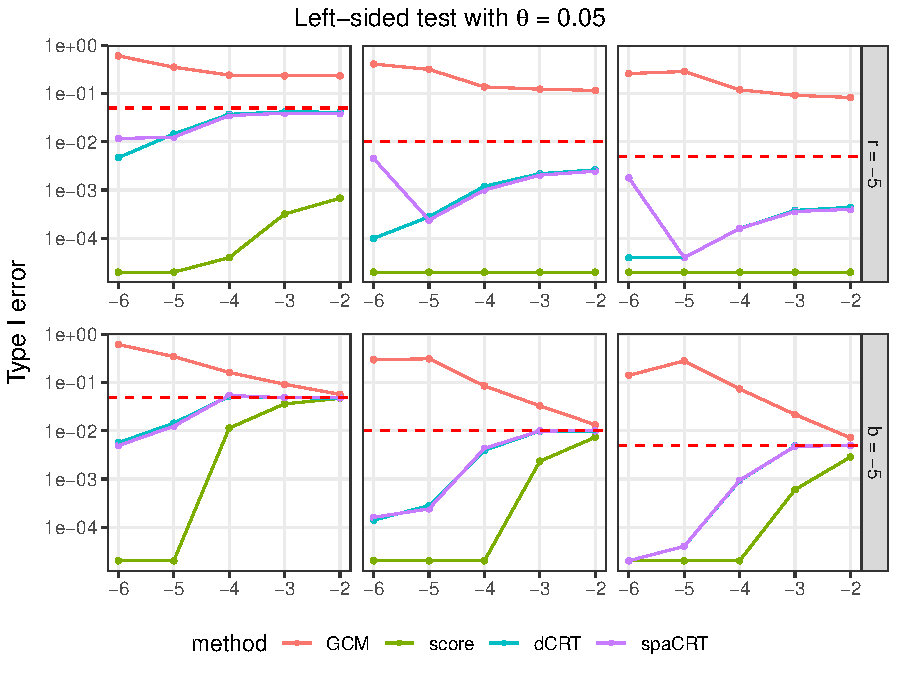
\includegraphics[width=0.95\textwidth]{figures-and-tables/simulation/Type-I-error/plot-bin-NB-normal-B-50000-n-5000-5e3-n5-n5-disp-5e-2-Type-I-error-LEFT.pdf}
  \end{subfigure}

  \begin{subfigure}{\textwidth}
    \centering
    %\includegraphics{figures-and-tables/simulation/QQ/QQ-LEFT/plot-bin-NB-normal-B-50000-n-5000-5e3-n5-n5-disp-5en2-QQ-LEFT.pdf}
    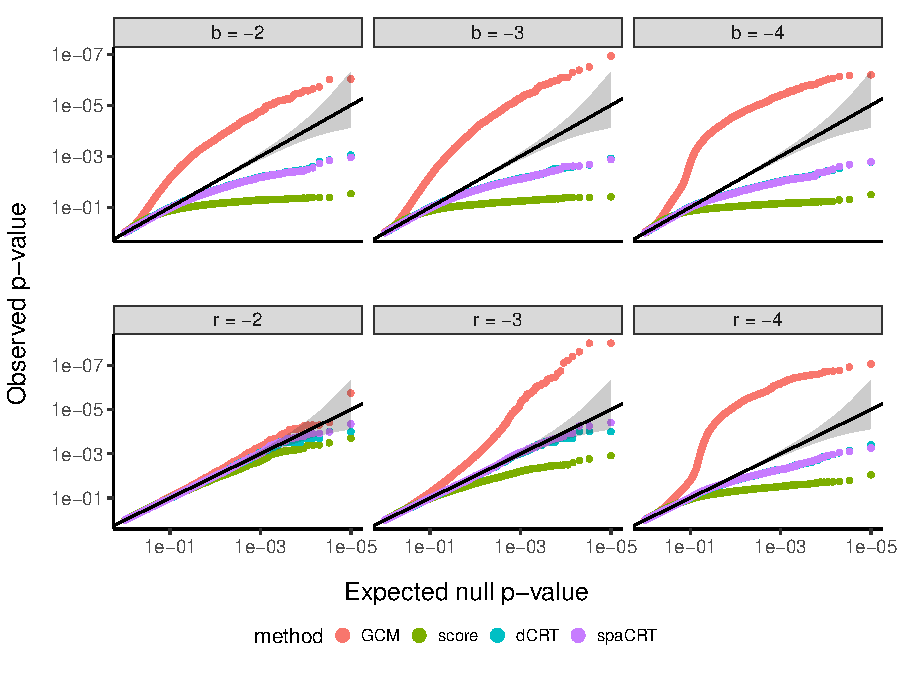
\includegraphics[width=0.95\textwidth]{figures-and-tables/simulation/QQ/plot-bin-NB-normal-B-50000-n-5000-5e3-n5-n5-disp-5e-2-QQ-LEFT.pdf}
  \end{subfigure}
  \caption{Type-I error plot and QQ-plots for the left-sided tests, with $\theta = 0.05$.}
  \label{fig:simulation-Type-I-error-LEFT-0.05}
\end{figure}


\begin{figure}[!ht]
  \centering
  \begin{subfigure}{\textwidth}
    \centering
    %\includegraphics{figures-and-tables/simulation/Type-I-error/RIGHT/plot-bin-NB-normal-B-50000-n-5000-5e3-n5-n5-disp-5en2-Type-I-eror-RIGHT.pdf}
    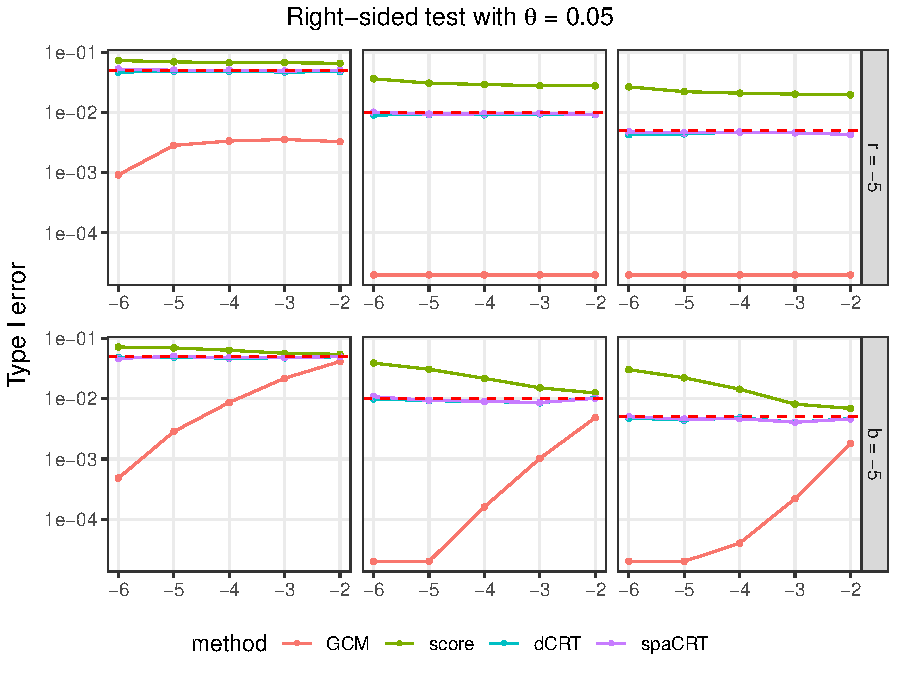
\includegraphics[width=0.95\textwidth]{figures-and-tables/simulation/Type-I-error/plot-bin-NB-normal-B-50000-n-5000-5e3-n5-n5-disp-5e-2-Type-I-error-RIGHT.pdf}
  \end{subfigure}

  \begin{subfigure}{\textwidth}
    \centering
    %\includegraphics{figures-and-tables/simulation/QQ/QQ-RIGHT/plot-bin-NB-normal-B-50000-n-5000-5e3-n5-n5-disp-5en2-QQ-RIGHT.pdf}
    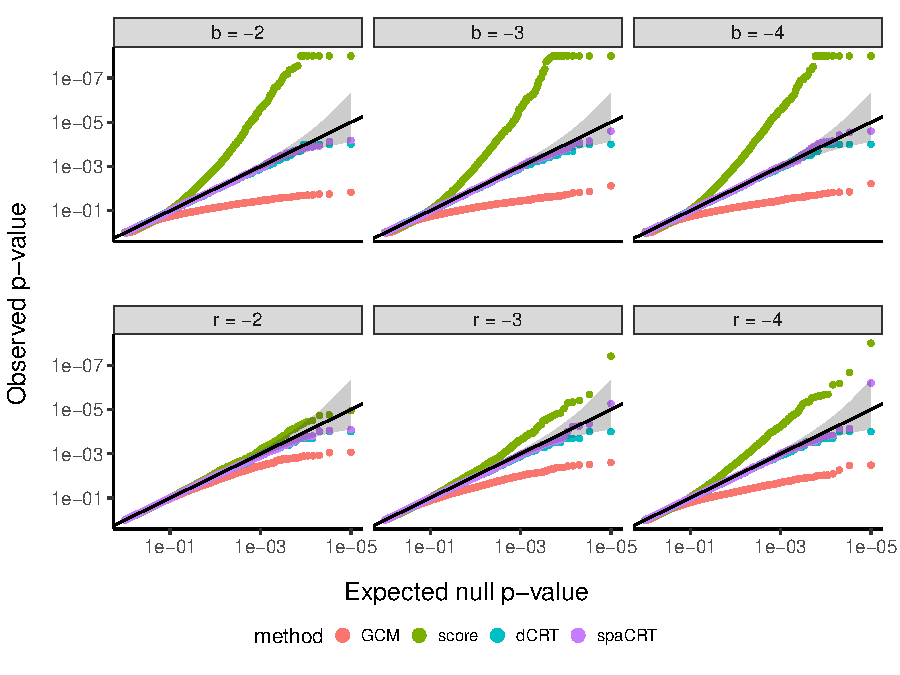
\includegraphics[width=0.95\textwidth]{figures-and-tables/simulation/QQ/plot-bin-NB-normal-B-50000-n-5000-5e3-n5-n5-disp-5e-2-QQ-RIGHT.pdf}
  \end{subfigure}
  \caption{Type-I error and QQ-plots for the right-sided tests, with $\theta = 0.05$.}
  \label{fig:simulation-Type-I-error-RIGHT-0.05}
\end{figure}

\begin{figure*}
  \centering
  \begin{subfigure}{\textwidth}
    \centering
    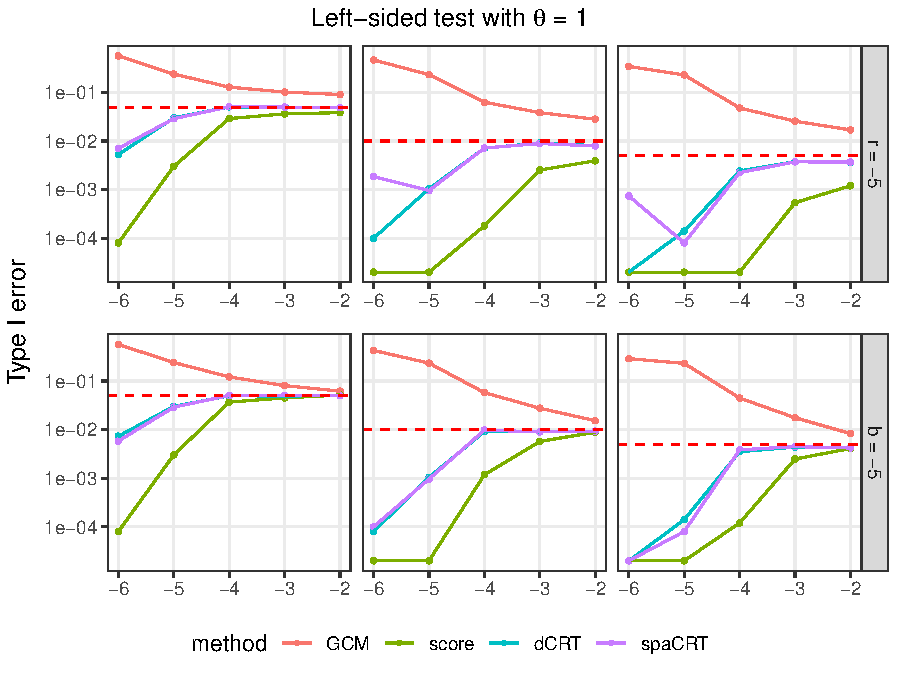
\includegraphics[width=0.95\textwidth]{figures-and-tables/simulation/Type-I-error/plot-bin-NB-normal-B-50000-n-5000-5e3-n5-n5-disp-1-Type-I-error-LEFT.pdf}
  \end{subfigure}

  \begin{subfigure}{\textwidth}
    \centering
    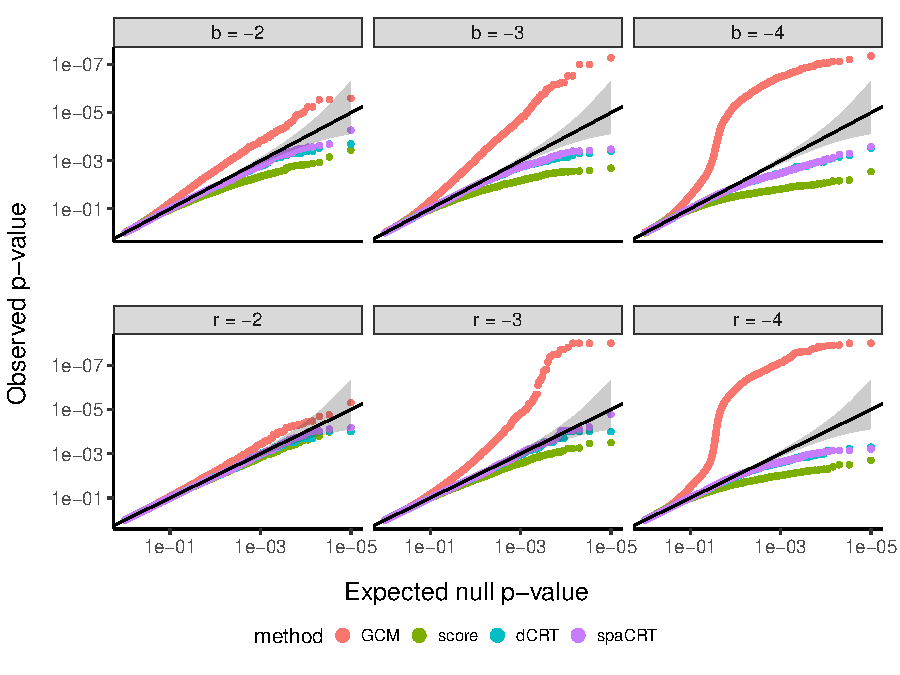
\includegraphics[width=0.95\textwidth]{figures-and-tables/simulation/QQ/plot-bin-NB-normal-B-50000-n-5000-5e3-n5-n5-disp-1-QQ-LEFT.pdf}
  \end{subfigure}
  \caption{Type-I error and QQ-plots for the left-sided tests, with $\theta = 1$.}
  \label{fig:simulation-Type-I-error-LEFT-1}
\end{figure*}

\begin{figure*}
  \centering
  \begin{subfigure}{\textwidth}
    \centering
    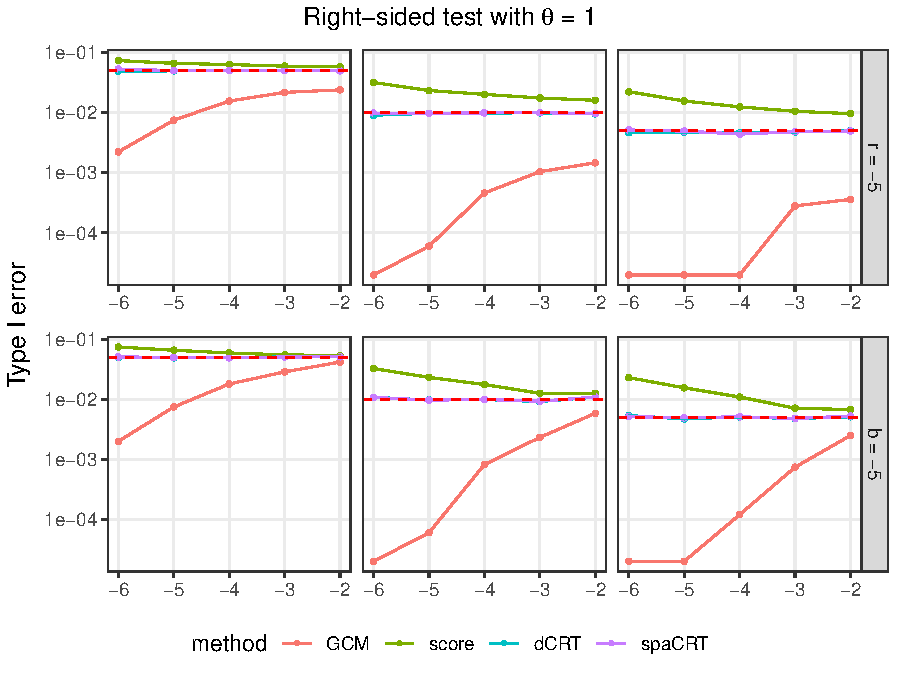
\includegraphics[width=0.95\textwidth]{figures-and-tables/simulation/Type-I-error/plot-bin-NB-normal-B-50000-n-5000-5e3-n5-n5-disp-1-Type-I-error-RIGHT.pdf}
  \end{subfigure}

  \begin{subfigure}{\textwidth}
    \centering
    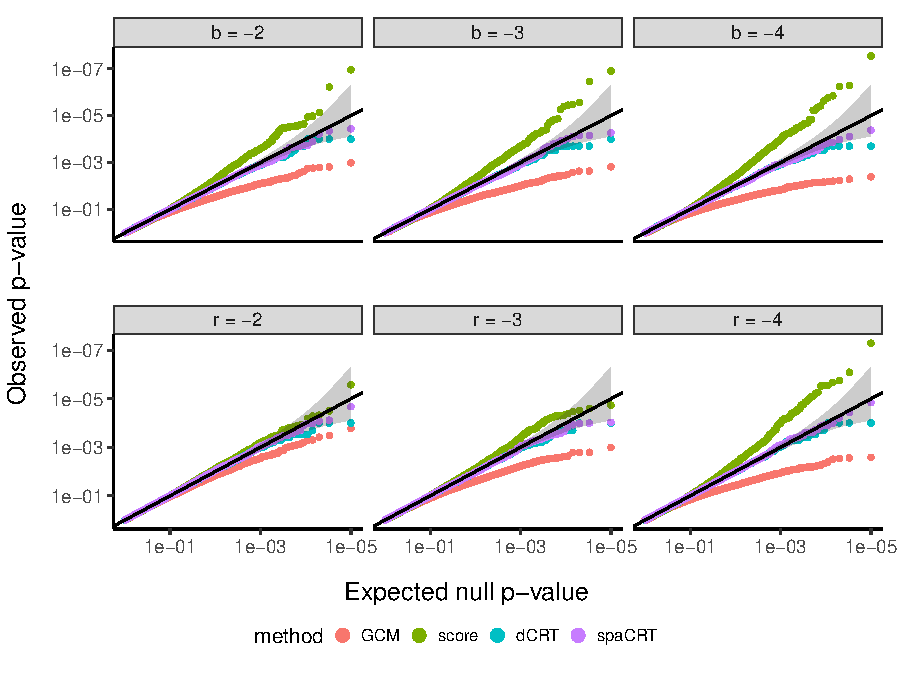
\includegraphics[width=0.95\textwidth]{figures-and-tables/simulation/QQ/plot-bin-NB-normal-B-50000-n-5000-5e3-n5-n5-disp-1-QQ-RIGHT.pdf}
  \end{subfigure}
  \caption{Type-I error and QQ-plots for the right-sided tests, with $\theta = 1$.}
  \label{fig:simulation-Type-I-error-RIGHT-1}
\end{figure*}

\begin{figure*}
  \centering
  \begin{subfigure}{\textwidth}
    \centering
    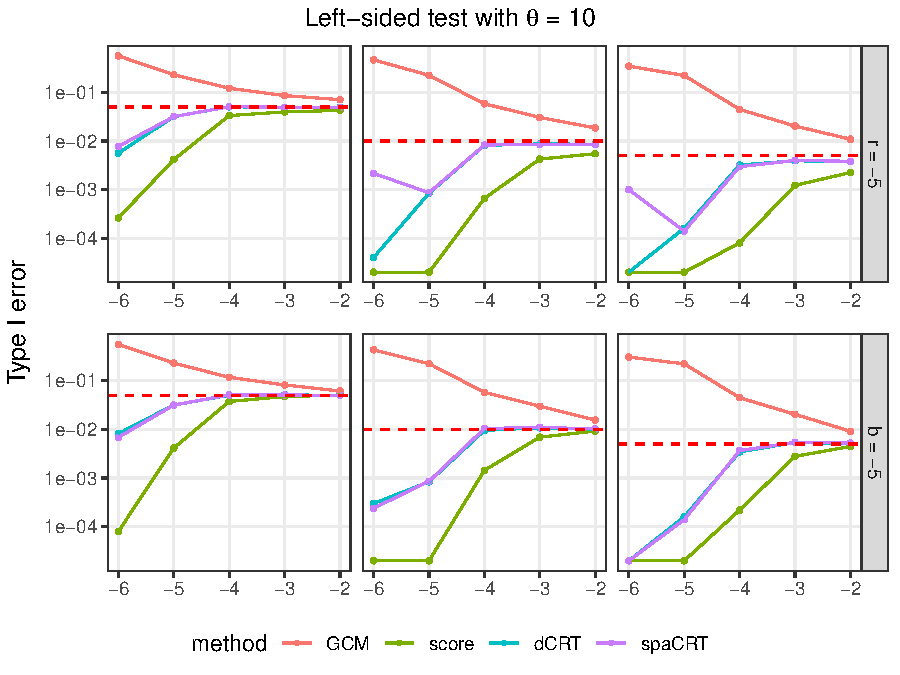
\includegraphics[width=0.95\textwidth]{figures-and-tables/simulation/Type-I-error/plot-bin-NB-normal-B-50000-n-5000-5e3-n5-n5-disp-10-Type-I-error-LEFT.pdf}
  \end{subfigure}

  \begin{subfigure}{\textwidth}
    \centering
    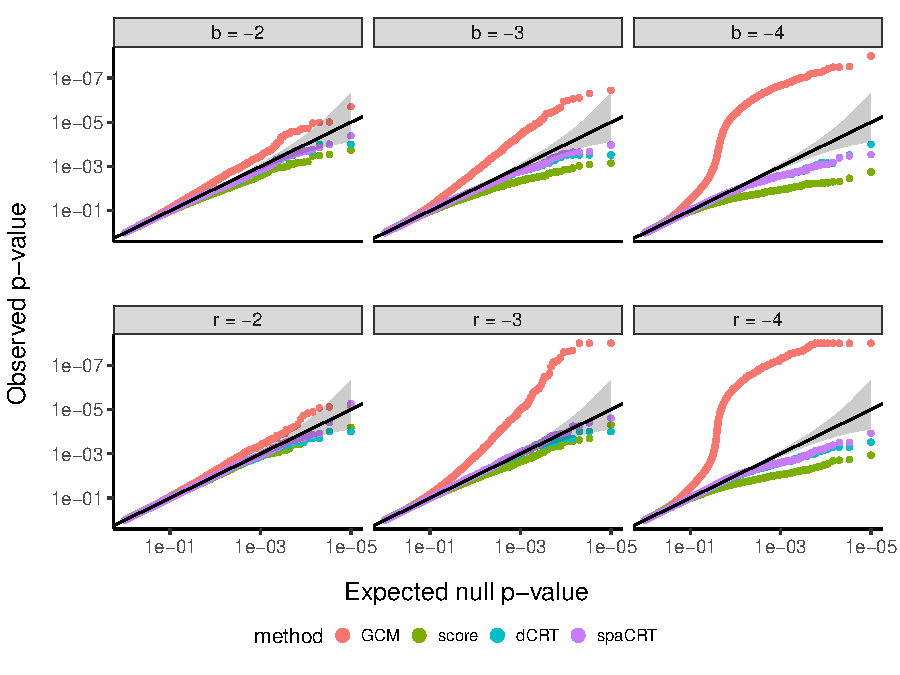
\includegraphics[width=0.95\textwidth]{figures-and-tables/simulation/QQ/plot-bin-NB-normal-B-50000-n-5000-5e3-n5-n5-disp-10-QQ-LEFT.pdf}
  \end{subfigure}
  \caption{Type-I error and QQ-plots for the left-sided tests, with $\theta = 10$.}
  \label{fig:simulation-Type-I-error-LEFT-10}
\end{figure*}

\begin{figure*}
  \centering
  \begin{subfigure}{\textwidth}
    \centering
    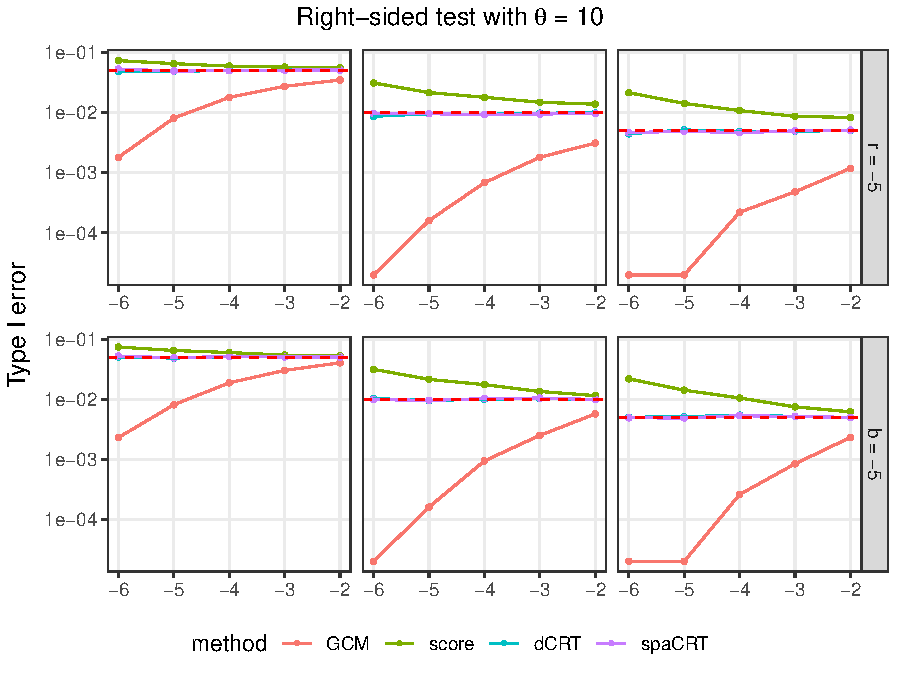
\includegraphics[width=0.95\textwidth]{figures-and-tables/simulation/Type-I-error/plot-bin-NB-normal-B-50000-n-5000-5e3-n5-n5-disp-10-Type-I-error-RIGHT.pdf}
  \end{subfigure}

  \begin{subfigure}{\textwidth}
    \centering
    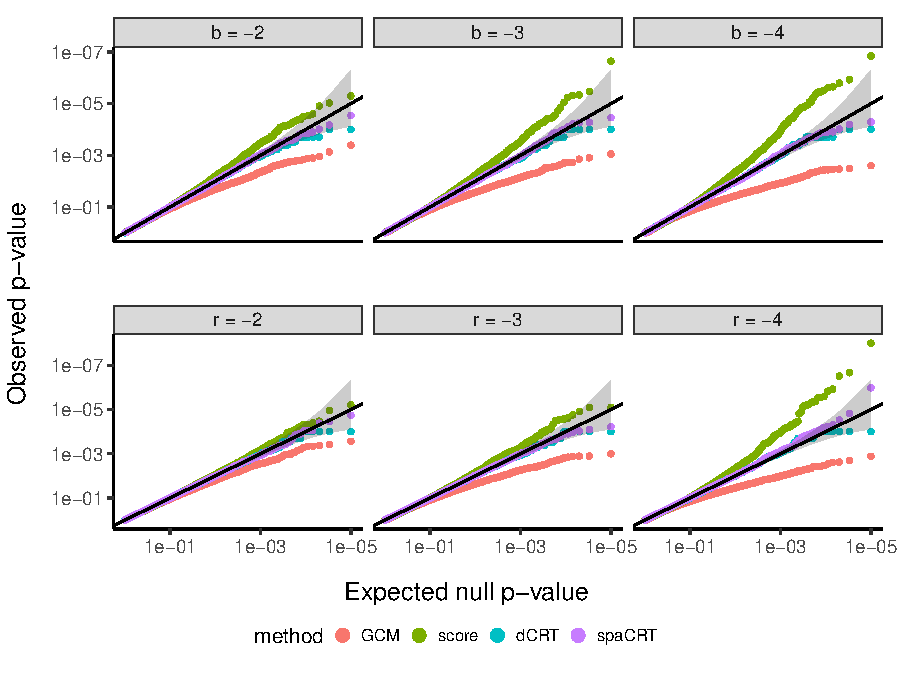
\includegraphics[width=0.95\textwidth]{figures-and-tables/simulation/QQ/plot-bin-NB-normal-B-50000-n-5000-5e3-n5-n5-disp-10-QQ-RIGHT.pdf}
  \end{subfigure}
  \caption{Type-I error and QQ-plots for the right-sided tests, with $\theta = 10$.}
  \label{fig:simulation-Type-I-error-RIGHT-10}
\end{figure*}

\begin{figure*}
  \centering

  \begin{subfigure}{\textwidth}
    \centering
    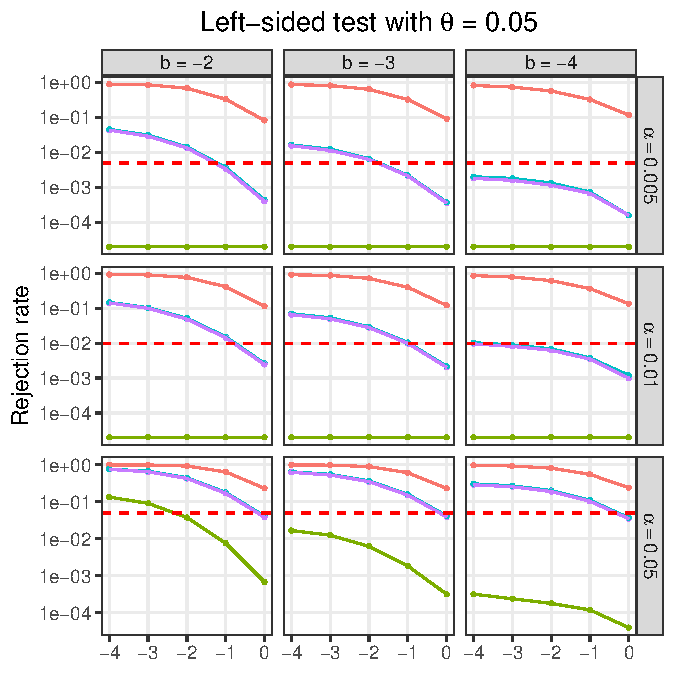
\includegraphics[width=0.72\textwidth]{figures-and-tables/simulation/power/plot-bin-NB-normal-B-50000-n-5000-5e3-n5-n5-disp-5e-2-power-fixed-gamma-LEFT.pdf}
  \end{subfigure}

  \begin{subfigure}{\textwidth}
    \centering
    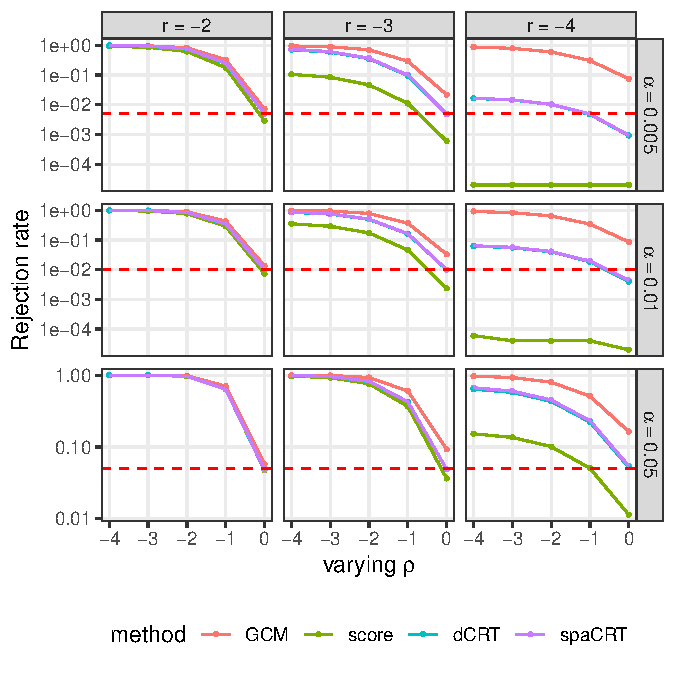
\includegraphics[width=0.72\textwidth]{figures-and-tables/simulation/power/plot-bin-NB-normal-B-50000-n-5000-5e3-n5-n5-disp-5e-2-power-fixed-beta-LEFT.pdf}
  \end{subfigure}

  \caption{Power plots for the left-sided tests, with $\theta = 0.05$.}
  \label{fig:simulation-power-LEFT-0.05}
\end{figure*}


\begin{figure*}
  \centering
  \begin{subfigure}{\textwidth}
    \centering
    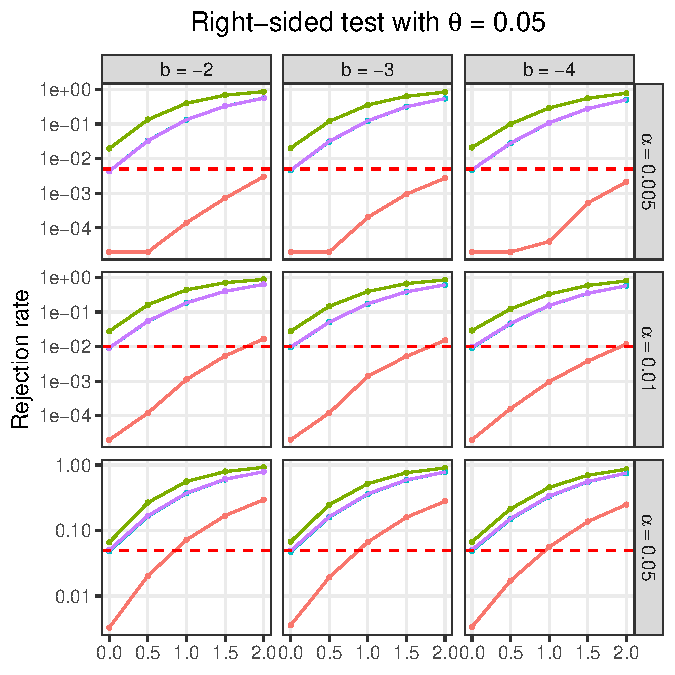
\includegraphics[width=0.72\textwidth]{figures-and-tables/simulation/power/plot-bin-NB-normal-B-50000-n-5000-5e3-n5-n5-disp-5e-2-power-fixed-gamma-RIGHT.pdf}
  \end{subfigure}

  \begin{subfigure}{\textwidth}
    \centering
    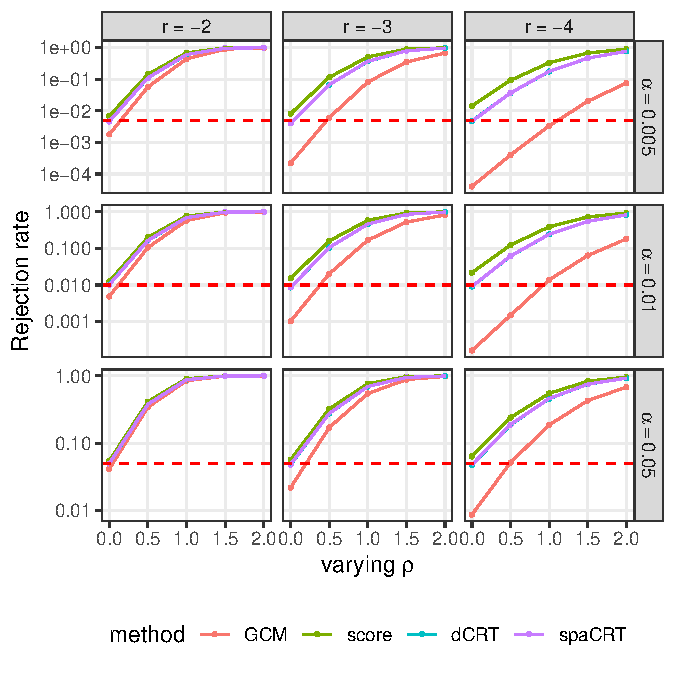
\includegraphics[width=0.72\textwidth]{figures-and-tables/simulation/power/plot-bin-NB-normal-B-50000-n-5000-5e3-n5-n5-disp-5e-2-power-fixed-beta-RIGHT.pdf}
  \end{subfigure}

  \caption{Power plots for the right-sided tests, with $\theta = 0.05$.}
  \label{fig:simulation-power-RIGHT-0.05}
\end{figure*}

\begin{figure*}
  \centering
  \begin{subfigure}{\textwidth}
    \centering
    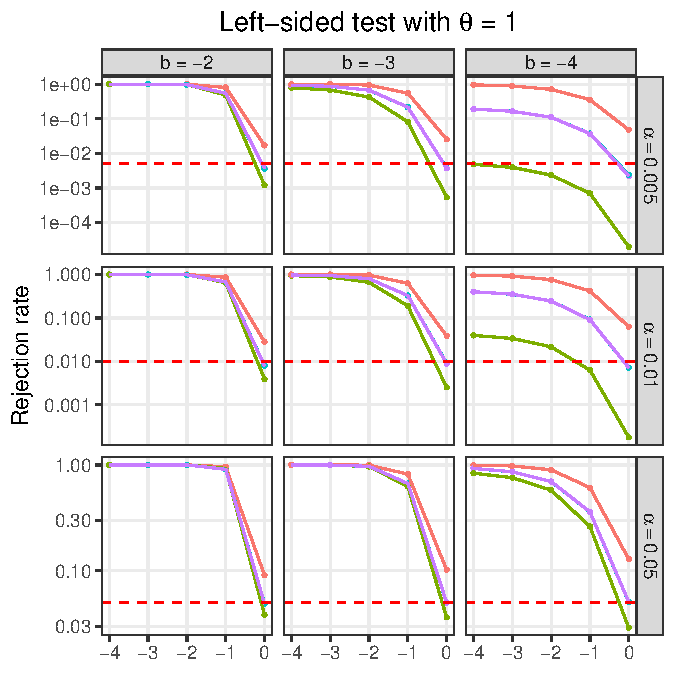
\includegraphics[width=0.72\textwidth]{figures-and-tables/simulation/power/plot-bin-NB-normal-B-50000-n-5000-5e3-n5-n5-disp-1-power-fixed-gamma-LEFT.pdf}
  \end{subfigure}

  \begin{subfigure}{\textwidth}
    \centering
    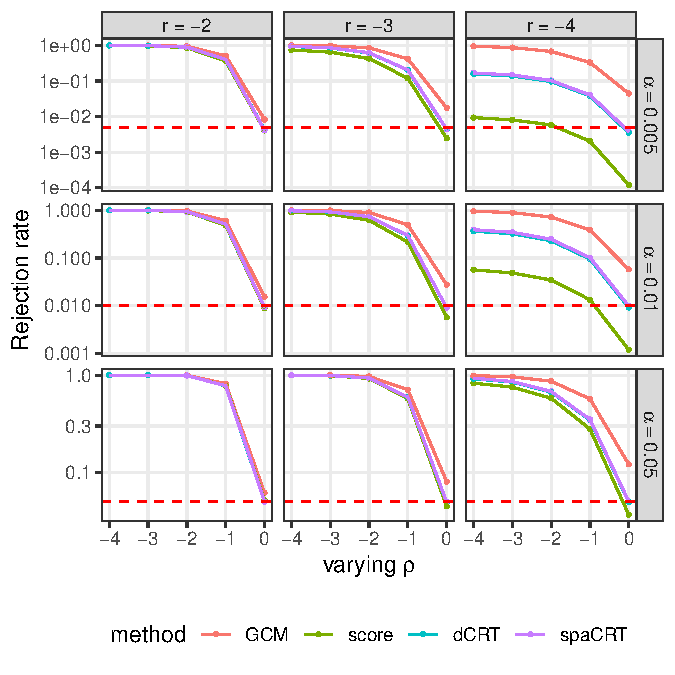
\includegraphics[width=0.72\textwidth]{figures-and-tables/simulation/power/plot-bin-NB-normal-B-50000-n-5000-5e3-n5-n5-disp-1-power-fixed-beta-LEFT.pdf}
  \end{subfigure}

  \caption{Power plots for the left-sided tests, with $\theta = 1$.}
  \label{fig:simulation-power-LEFT-1}
\end{figure*}


\begin{figure*}
  \centering
  \begin{subfigure}{\textwidth}
    \centering
    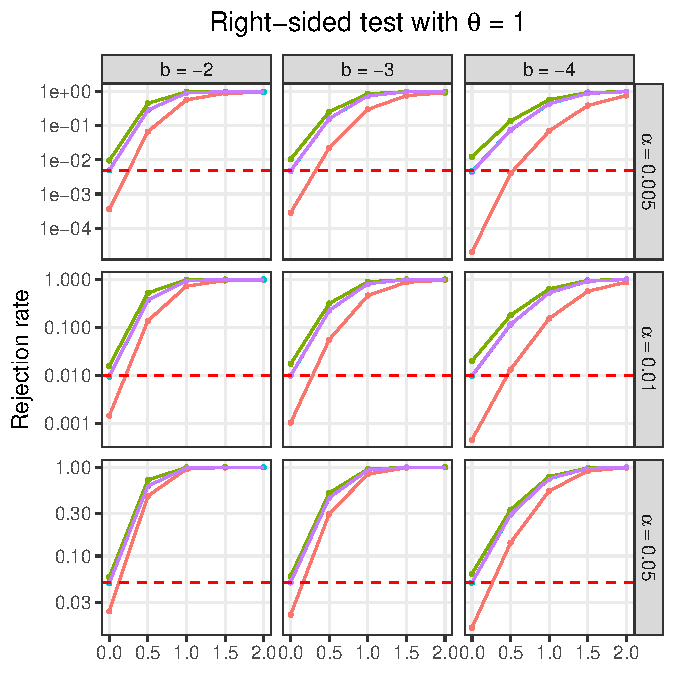
\includegraphics[width=0.72\textwidth]{figures-and-tables/simulation/power/plot-bin-NB-normal-B-50000-n-5000-5e3-n5-n5-disp-1-power-fixed-gamma-RIGHT.pdf}
  \end{subfigure}

  \begin{subfigure}{\textwidth}
    \centering
    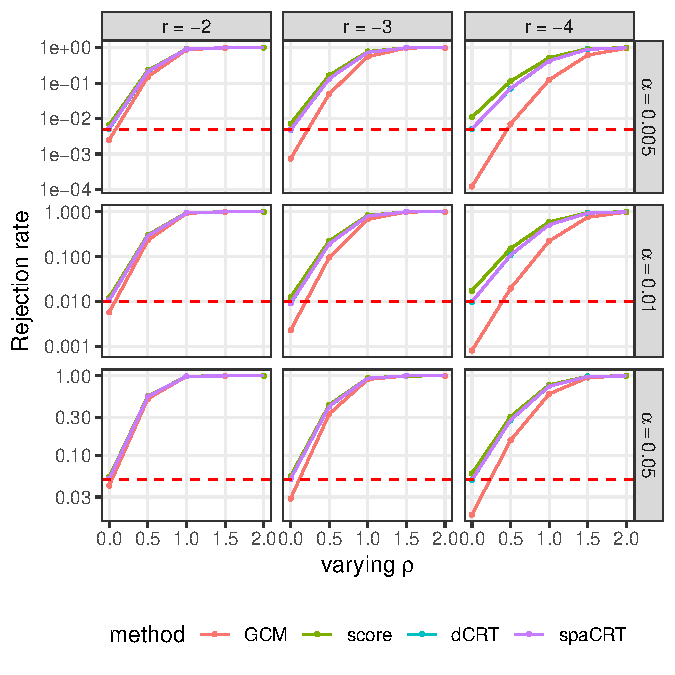
\includegraphics[width=0.72\textwidth]{figures-and-tables/simulation/power/plot-bin-NB-normal-B-50000-n-5000-5e3-n5-n5-disp-1-power-fixed-beta-RIGHT.pdf}
  \end{subfigure}

  \caption{Power plots for the right-sided tests, with $\theta = 1$.}
  \label{fig:simulation-power-RIGHT-1}
\end{figure*}


\begin{figure*}
  \centering

  \begin{subfigure}{\textwidth}
    \centering
    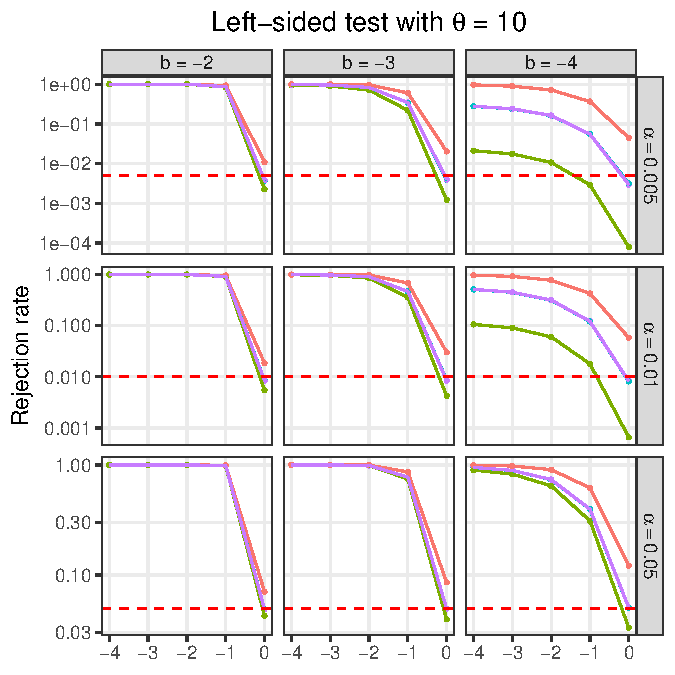
\includegraphics[width=0.72\textwidth]{figures-and-tables/simulation/power/plot-bin-NB-normal-B-50000-n-5000-5e3-n5-n5-disp-10-power-fixed-gamma-LEFT.pdf}
  \end{subfigure}

  \begin{subfigure}{\textwidth}
    \centering
    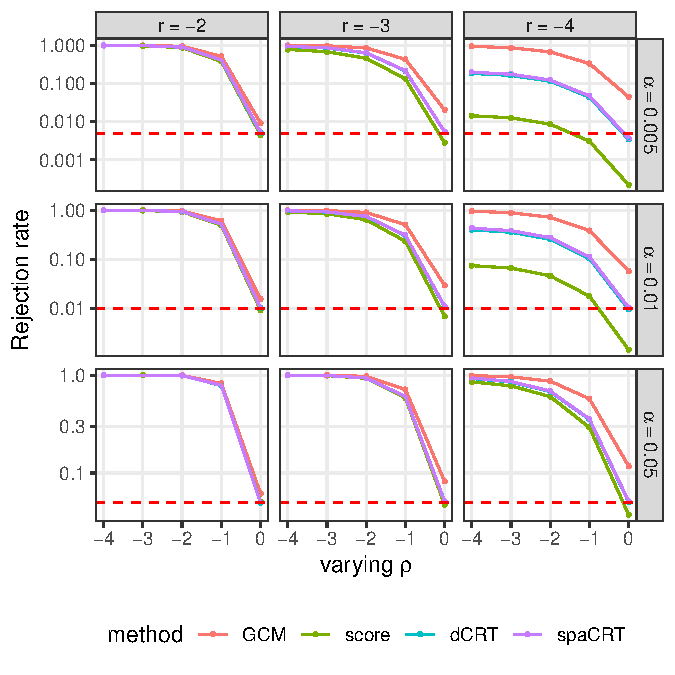
\includegraphics[width=0.72\textwidth]{figures-and-tables/simulation/power/plot-bin-NB-normal-B-50000-n-5000-5e3-n5-n5-disp-10-power-fixed-beta-LEFT.pdf}
  \end{subfigure}

  \caption{Power plots for the left-sided tests, with $\theta = 10$.}
  \label{fig:simulation-power-LEFT-10}
\end{figure*}


\begin{figure*}
  \centering
  \begin{subfigure}{\textwidth}
    \centering
    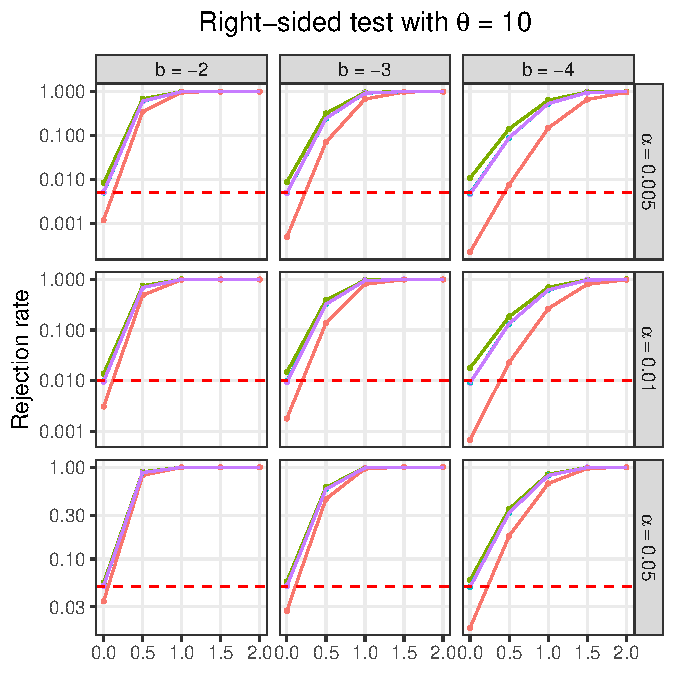
\includegraphics[width=0.72\textwidth]{figures-and-tables/simulation/power/plot-bin-NB-normal-B-50000-n-5000-5e3-n5-n5-disp-10-power-fixed-gamma-RIGHT.pdf}
  \end{subfigure}

  \begin{subfigure}{\textwidth}
    \centering
    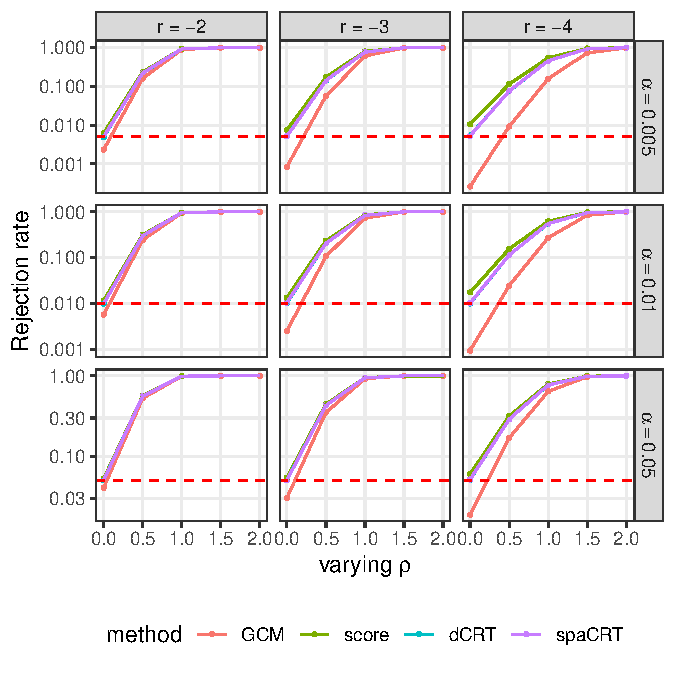
\includegraphics[width=0.72\textwidth]{figures-and-tables/simulation/power/plot-bin-NB-normal-B-50000-n-5000-5e3-n5-n5-disp-10-power-fixed-beta-RIGHT.pdf}
  \end{subfigure}

  \caption{Power plots for the right-sided tests, with $\theta = 10$.}
  \label{fig:simulation-power-RIGHT-10}
\end{figure*}

\begin{figure*}
  \centering
  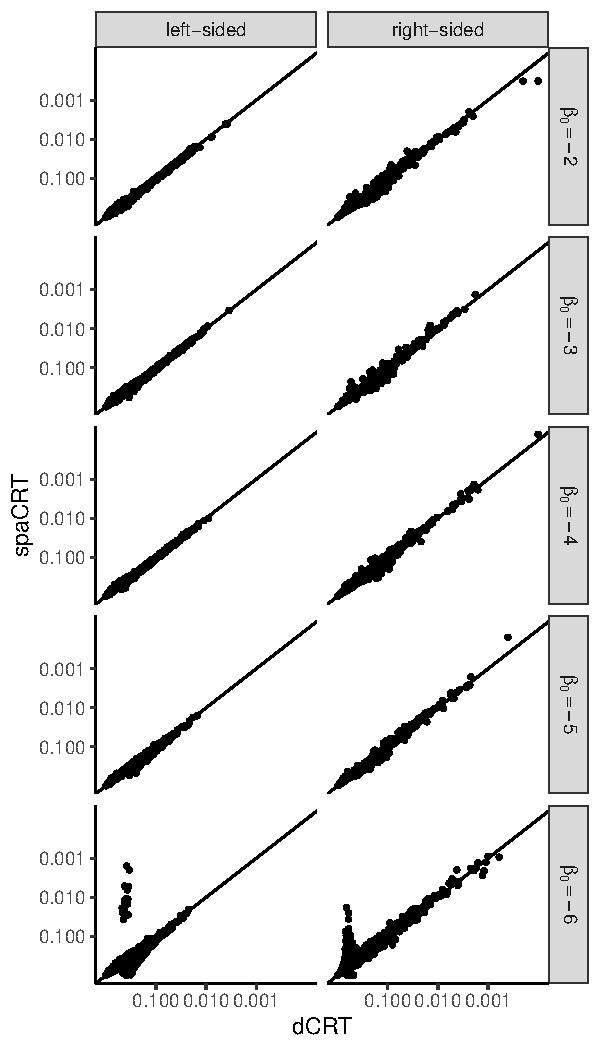
\includegraphics[width=0.8\textwidth]{figures-and-tables/simulation/QQ/plot-bin-NB-normal-B-50000-n-5000-5e3-n5-n5-disp-5e-2full-dCRT-spaCRT-varying-beta.pdf}
  \caption{Scatter plots for the $p$-values of the left-sided and right-sided tests when varying $\beta_0\in \{-6,-5,-4,-3,-2\}$ and fixing $\gamma_0=-5$, with $\theta = 0.05$.}
  \label{fig:simulation-dot-plot-varying-beta-theta-0.05}
\end{figure*}


\begin{figure*}
  \centering
  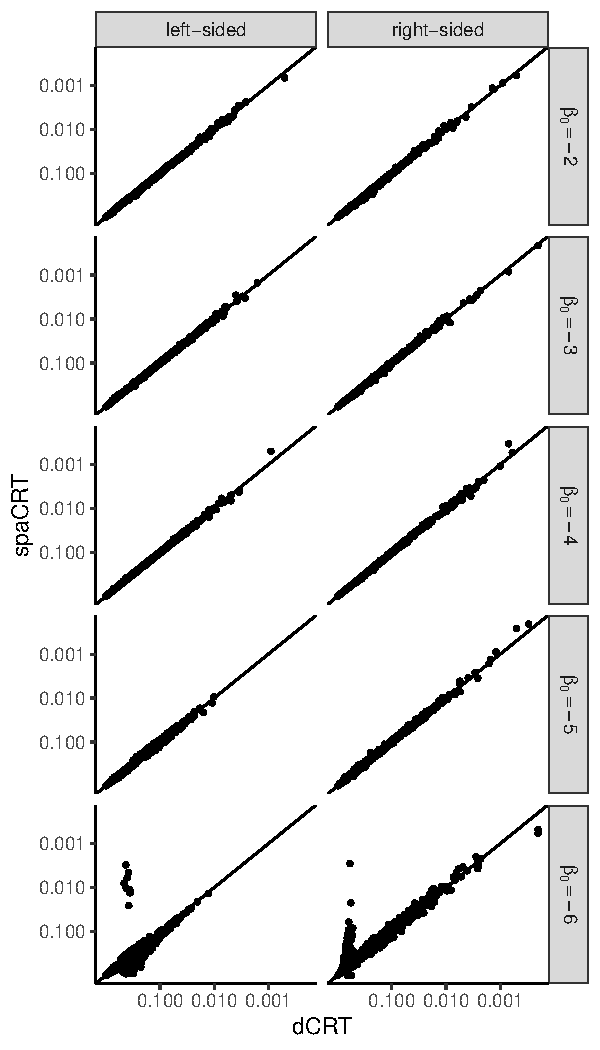
\includegraphics[width=0.8\textwidth]{figures-and-tables/simulation/QQ/plot-bin-NB-normal-B-50000-n-5000-5e3-n5-n5-disp-1full-dCRT-spaCRT-varying-beta.pdf}
  \caption{Scatter plots for the $p$-values of the left-sided and right-sided tests when varying $\beta_0\in \{-6,-5,-4,-3,-2\}$ and fixing $\gamma_0=-5$, with $\theta = 1$.}
  \label{fig:simulation-dot-plot-varying-beta-theta-1}
\end{figure*}

\begin{figure*}
  \centering
  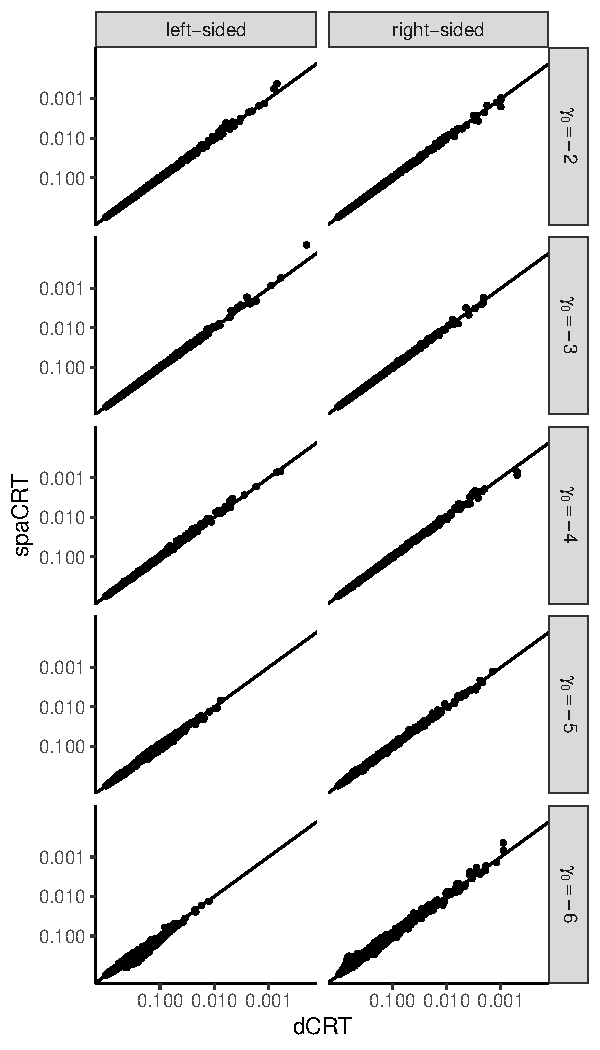
\includegraphics[width=0.8\textwidth]{figures-and-tables/simulation/QQ/plot-bin-NB-normal-B-50000-n-5000-5e3-n5-n5-disp-1full-dCRT-spaCRT-varying-gamma.pdf}
  \caption{Scatter plots for the $p$-values of the left-sided and right-sided tests when varying $\gamma_0\in \{-6,-5,-4,-3,-2\}$ and fixing $\beta_0=-5$, with $\theta = 1$.}
  \label{fig:simulation-dot-plot-varying-gamma-theta-1}
\end{figure*}

\begin{figure*}
  \centering
  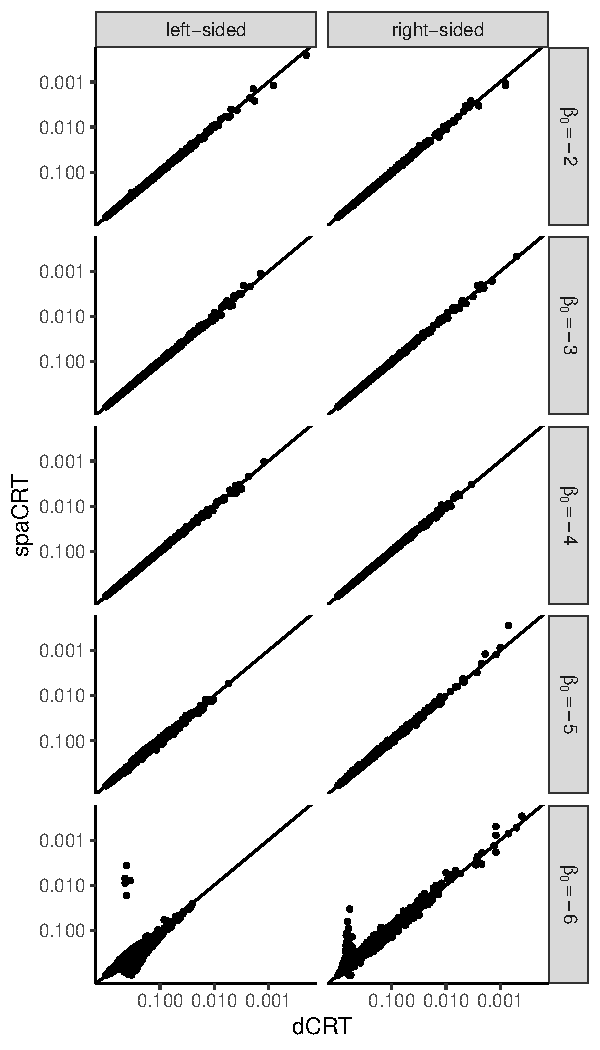
\includegraphics[width=0.8\textwidth]{figures-and-tables/simulation/QQ/plot-bin-NB-normal-B-50000-n-5000-5e3-n5-n5-disp-10full-dCRT-spaCRT-varying-beta.pdf}
  \caption{Scatter plots for the $p$-values of the left-sided and right-sided tests when varying $\beta_0\in \{-6,-5,-4,-3,-2\}$ and fixing $\gamma_0=-5$, with $\theta = 10$.}
  \label{fig:simulation-dot-plot-varying-beta-theta-10}
\end{figure*}

\begin{figure*}
  \centering
  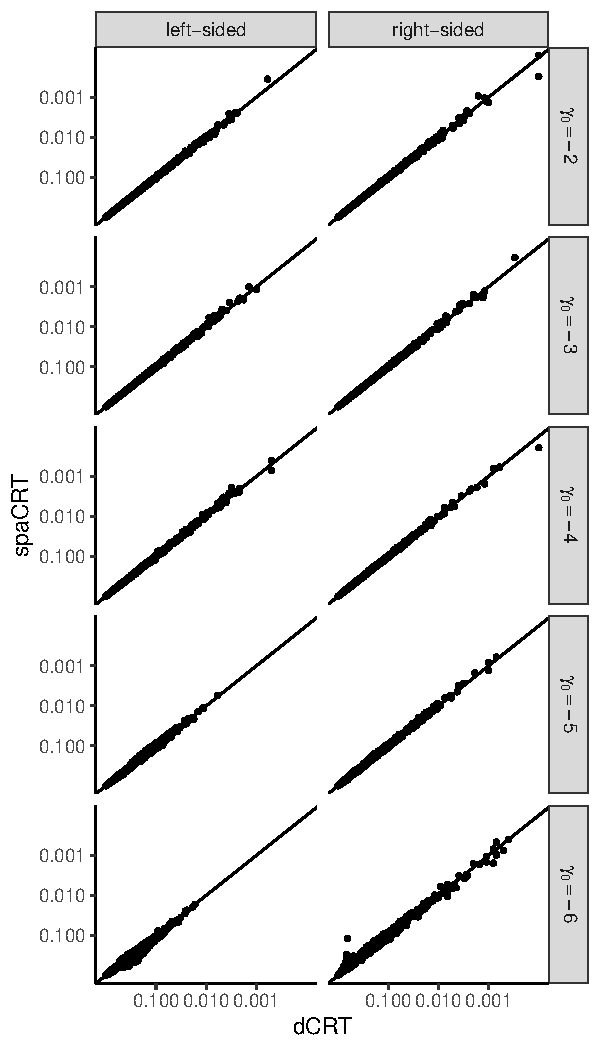
\includegraphics[width=0.8\textwidth]{figures-and-tables/simulation/QQ/plot-bin-NB-normal-B-50000-n-5000-5e3-n5-n5-disp-10full-dCRT-spaCRT-varying-gamma.pdf}
  \caption{Scatter plots for the $p$-values of the left-sided and right-sided tests when varying $\gamma_0\in \{-6,-5,-4,-3,-2\}$ and fixing $\beta_0=-5$, with $\theta = 10$.}
  \label{fig:simulation-dot-plot-varying-gamma-theta-10}
\end{figure*}


\newpage

\subsection{Additional tables for the simulation study}\label{sec:additional_table_simulation}

{\color{red}

In this section, we compute the number of rejections by first applying the four single testing methods considered in section \ref{sec:simulation} and then applying either Bonferroni or Benjamini-Hochberg (BH) method to the obtained $p$-values. In order to do so, we regroup the $50000$ replications to $50$ independent simulation groups with each group including $5000$ independent $p$-values. In particular, we only consider the null setup ($\rho=0$) and $\theta=0.05$. Thus we will expect the number of rejections will be very close to $0$ after multiplicity correction and the final results are presented in the following tables.
}

\begin{table}[!h]
\centering
\caption{\label{tab:simulation_rejection_beta_-6_gamma_-5}Number of rejections when $(\beta_0,\gamma_0,\rho) = (-6, -5, 0)$.}
\centering
\begin{tabular}[t]{lrrrr}
\toprule
\multicolumn{1}{c}{ } & \multicolumn{4}{c}{Number of rejections} \\
\cmidrule(l{3pt}r{3pt}){2-5}
\multicolumn{1}{c}{ } & \multicolumn{2}{c}{Left-sided test} & \multicolumn{2}{c}{Right-sided test} \\
\cmidrule(l{3pt}r{3pt}){2-3} \cmidrule(l{3pt}r{3pt}){4-5}
\multicolumn{1}{c}{Method} & \multicolumn{1}{c}{Bonferroni} & \multicolumn{1}{c}{BH} & \multicolumn{1}{c}{Bonferroni} & \multicolumn{1}{c}{BH} \\
\cmidrule(l{3pt}r{3pt}){1-1} \cmidrule(l{3pt}r{3pt}){2-2} \cmidrule(l{3pt}r{3pt}){3-3} \cmidrule(l{3pt}r{3pt}){4-4} \cmidrule(l{3pt}r{3pt}){5-5}
GCM test & 0 & 607.6 & 0.0 & 0.0\\
Score test & 0 & 0.0 & 5.6 & 17.8\\
dCRT & 0 & 0.0 & 0.1 & 0.1\\
spaCRT & 0 & 0.0 & 0.1 & 0.1\\
\bottomrule
\end{tabular}
\end{table}


\begin{table}[!h]
\centering
\caption{\label{tab:simulation_rejection_beta_-5_gamma_-6}Number of rejections when $(\beta_0,\gamma_0,\rho) = (-5, -6, 0)$.}
\centering
\begin{tabular}[t]{lrrrr}
\toprule
\multicolumn{1}{c}{ } & \multicolumn{4}{c}{Number of rejections} \\
\cmidrule(l{3pt}r{3pt}){2-5}
\multicolumn{1}{c}{ } & \multicolumn{2}{c}{Left-sided test} & \multicolumn{2}{c}{Right-sided test} \\
\cmidrule(l{3pt}r{3pt}){2-3} \cmidrule(l{3pt}r{3pt}){4-5}
\multicolumn{1}{c}{Method} & \multicolumn{1}{c}{Bonferroni} & \multicolumn{1}{c}{BH} & \multicolumn{1}{c}{Bonferroni} & \multicolumn{1}{c}{BH} \\
\cmidrule(l{3pt}r{3pt}){1-1} \cmidrule(l{3pt}r{3pt}){2-2} \cmidrule(l{3pt}r{3pt}){3-3} \cmidrule(l{3pt}r{3pt}){4-4} \cmidrule(l{3pt}r{3pt}){5-5}
GCM test & 0 & 642.4 & 0.0 & 0.0\\
Score test & 0 & 0.0 & 10.5 & 24.2\\
dCRT & 0 & 0.0 & 0.1 & 0.1\\
spaCRT & 0 & 0.0 & 0.0 & 0.1\\
\bottomrule
\end{tabular}
\end{table}


\begin{table}[!h]
\centering
\caption{\label{tab:simulation_rejection_beta_-5_gamma_-5}Number of rejections when $(\beta_0,\gamma_0,\rho) = (-5, -5, 0)$.}
\centering
\begin{tabular}[t]{lrrrr}
\toprule
\multicolumn{1}{c}{ } & \multicolumn{4}{c}{Number of rejections} \\
\cmidrule(l{3pt}r{3pt}){2-5}
\multicolumn{1}{c}{ } & \multicolumn{2}{c}{Left-sided test} & \multicolumn{2}{c}{Right-sided test} \\
\cmidrule(l{3pt}r{3pt}){2-3} \cmidrule(l{3pt}r{3pt}){4-5}
\multicolumn{1}{c}{Method} & \multicolumn{1}{c}{Bonferroni} & \multicolumn{1}{c}{BH} & \multicolumn{1}{c}{Bonferroni} & \multicolumn{1}{c}{BH} \\
\cmidrule(l{3pt}r{3pt}){1-1} \cmidrule(l{3pt}r{3pt}){2-2} \cmidrule(l{3pt}r{3pt}){3-3} \cmidrule(l{3pt}r{3pt}){4-4} \cmidrule(l{3pt}r{3pt}){5-5}
GCM test & 19.2 & 343 & 0.0 & 0.0\\
Score test & 0.0 & 0 & 4.5 & 11.9\\
dCRT & 0.0 & 0 & 0.1 & 0.1\\
spaCRT & 0.0 & 0 & 0.1 & 0.1\\
\bottomrule
\end{tabular}
\end{table}


\begin{table}[!h]
\centering
\caption{\label{tab:simulation_rejection_beta_-5_gamma_-4}Number of rejections when $(\beta_0,\gamma_0,\rho) = (-5, -4, 0)$.}
\centering
\begin{tabular}[t]{lrrrr}
\toprule
\multicolumn{1}{c}{ } & \multicolumn{4}{c}{Number of rejections} \\
\cmidrule(l{3pt}r{3pt}){2-5}
\multicolumn{1}{c}{ } & \multicolumn{2}{c}{Left-sided test} & \multicolumn{2}{c}{Right-sided test} \\
\cmidrule(l{3pt}r{3pt}){2-3} \cmidrule(l{3pt}r{3pt}){4-5}
\multicolumn{1}{c}{Method} & \multicolumn{1}{c}{Bonferroni} & \multicolumn{1}{c}{BH} & \multicolumn{1}{c}{Bonferroni} & \multicolumn{1}{c}{BH} \\
\cmidrule(l{3pt}r{3pt}){1-1} \cmidrule(l{3pt}r{3pt}){2-2} \cmidrule(l{3pt}r{3pt}){3-3} \cmidrule(l{3pt}r{3pt}){4-4} \cmidrule(l{3pt}r{3pt}){5-5}
GCM test & 38.8 & 82 & 0.0 & 0.0\\
Score test & 0.0 & 0 & 1.5 & 3.6\\
dCRT & 0.0 & 0 & 0.1 & 0.1\\
spaCRT & 0.0 & 0 & 0.1 & 0.1\\
\bottomrule
\end{tabular}
\end{table}


\begin{table}[!h]
\centering
\caption{\label{tab:simulation_rejection_beta_-5_gamma_-3}Number of rejections when $(\beta_0,\gamma_0,\rho) = (-5, -3, 0)$.}
\centering
\begin{tabular}[t]{lrrrr}
\toprule
\multicolumn{1}{c}{ } & \multicolumn{4}{c}{Number of rejections} \\
\cmidrule(l{3pt}r{3pt}){2-5}
\multicolumn{1}{c}{ } & \multicolumn{2}{c}{Left-sided test} & \multicolumn{2}{c}{Right-sided test} \\
\cmidrule(l{3pt}r{3pt}){2-3} \cmidrule(l{3pt}r{3pt}){4-5}
\multicolumn{1}{c}{Method} & \multicolumn{1}{c}{Bonferroni} & \multicolumn{1}{c}{BH} & \multicolumn{1}{c}{Bonferroni} & \multicolumn{1}{c}{BH} \\
\cmidrule(l{3pt}r{3pt}){1-1} \cmidrule(l{3pt}r{3pt}){2-2} \cmidrule(l{3pt}r{3pt}){3-3} \cmidrule(l{3pt}r{3pt}){4-4} \cmidrule(l{3pt}r{3pt}){5-5}
GCM test & 3.0 & 8.8 & 0.0 & 0.0\\
Score test & 0.0 & 0.0 & 0.5 & 0.9\\
dCRT & 0.1 & 0.1 & 0.0 & 0.1\\
spaCRT & 0.1 & 0.1 & 0.1 & 0.1\\
\bottomrule
\end{tabular}
\end{table}


\begin{table}[!h]
\centering
\caption{\label{tab:simulation_rejection_beta_-5_gamma_-2}Number of rejections when $(\beta_0,\gamma_0,\rho) = (-5, -2, 0)$.}
\centering
\begin{tabular}[t]{lrrrr}
\toprule
\multicolumn{1}{c}{ } & \multicolumn{4}{c}{Number of rejections} \\
\cmidrule(l{3pt}r{3pt}){2-5}
\multicolumn{1}{c}{ } & \multicolumn{2}{c}{Left-sided test} & \multicolumn{2}{c}{Right-sided test} \\
\cmidrule(l{3pt}r{3pt}){2-3} \cmidrule(l{3pt}r{3pt}){4-5}
\multicolumn{1}{c}{Method} & \multicolumn{1}{c}{Bonferroni} & \multicolumn{1}{c}{BH} & \multicolumn{1}{c}{Bonferroni} & \multicolumn{1}{c}{BH} \\
\cmidrule(l{3pt}r{3pt}){1-1} \cmidrule(l{3pt}r{3pt}){2-2} \cmidrule(l{3pt}r{3pt}){3-3} \cmidrule(l{3pt}r{3pt}){4-4} \cmidrule(l{3pt}r{3pt}){5-5}
GCM test & 0.2 & 0.3 & 0.0 & 0.0\\
Score test & 0.0 & 0.0 & 0.2 & 0.3\\
dCRT & 0.0 & 0.1 & 0.1 & 0.1\\
spaCRT & 0.0 & 0.0 & 0.1 & 0.1\\
\bottomrule
\end{tabular}
\end{table}


\begin{table}[!h]
\centering
\caption{\label{tab:simulation_rejection_beta_-4_gamma_-5}Number of rejections when $(\beta_0,\gamma_0,\rho) = (-4, -5, 0)$.}
\centering
\begin{tabular}[t]{lrrrr}
\toprule
\multicolumn{1}{c}{ } & \multicolumn{4}{c}{Number of rejections} \\
\cmidrule(l{3pt}r{3pt}){2-5}
\multicolumn{1}{c}{ } & \multicolumn{2}{c}{Left-sided test} & \multicolumn{2}{c}{Right-sided test} \\
\cmidrule(l{3pt}r{3pt}){2-3} \cmidrule(l{3pt}r{3pt}){4-5}
\multicolumn{1}{c}{Method} & \multicolumn{1}{c}{Bonferroni} & \multicolumn{1}{c}{BH} & \multicolumn{1}{c}{Bonferroni} & \multicolumn{1}{c}{BH} \\
\cmidrule(l{3pt}r{3pt}){1-1} \cmidrule(l{3pt}r{3pt}){2-2} \cmidrule(l{3pt}r{3pt}){3-3} \cmidrule(l{3pt}r{3pt}){4-4} \cmidrule(l{3pt}r{3pt}){5-5}
GCM test & 30.8 & 154.1 & 0.0 & 0.0\\
Score test & 0.0 & 0.0 & 4.2 & 11.1\\
dCRT & 0.0 & 0.0 & 0.1 & 0.1\\
spaCRT & 0.0 & 0.0 & 0.2 & 0.2\\
\bottomrule
\end{tabular}
\end{table}


\begin{table}[!h]
\centering
\caption{\label{tab:simulation_rejection_beta_-3_gamma_-5}Number of rejections when $(\beta_0,\gamma_0,\rho) = (-3, -5, 0)$.}
\centering
\begin{tabular}[t]{lrrrr}
\toprule
\multicolumn{1}{c}{ } & \multicolumn{4}{c}{Number of rejections} \\
\cmidrule(l{3pt}r{3pt}){2-5}
\multicolumn{1}{c}{ } & \multicolumn{2}{c}{Left-sided test} & \multicolumn{2}{c}{Right-sided test} \\
\cmidrule(l{3pt}r{3pt}){2-3} \cmidrule(l{3pt}r{3pt}){4-5}
\multicolumn{1}{c}{Method} & \multicolumn{1}{c}{Bonferroni} & \multicolumn{1}{c}{BH} & \multicolumn{1}{c}{Bonferroni} & \multicolumn{1}{c}{BH} \\
\cmidrule(l{3pt}r{3pt}){1-1} \cmidrule(l{3pt}r{3pt}){2-2} \cmidrule(l{3pt}r{3pt}){3-3} \cmidrule(l{3pt}r{3pt}){4-4} \cmidrule(l{3pt}r{3pt}){5-5}
GCM test & 11.3 & 142 & 0.0 & 0.0\\
Score test & 0.0 & 0 & 3.9 & 10.5\\
dCRT & 0.0 & 0 & 0.1 & 0.1\\
spaCRT & 0.0 & 0 & 0.1 & 0.1\\
\bottomrule
\end{tabular}
\end{table}


\begin{table}[!h]
\centering
\caption{\label{tab:simulation_rejection_beta_-2_gamma_-5}Number of rejections when $(\beta_0,\gamma_0,\rho) = (-2, -5, 0)$.}
\centering
\begin{tabular}[t]{lrrrr}
\toprule
\multicolumn{1}{c}{ } & \multicolumn{4}{c}{Number of rejections} \\
\cmidrule(l{3pt}r{3pt}){2-5}
\multicolumn{1}{c}{ } & \multicolumn{2}{c}{Left-sided test} & \multicolumn{2}{c}{Right-sided test} \\
\cmidrule(l{3pt}r{3pt}){2-3} \cmidrule(l{3pt}r{3pt}){4-5}
\multicolumn{1}{c}{Method} & \multicolumn{1}{c}{Bonferroni} & \multicolumn{1}{c}{BH} & \multicolumn{1}{c}{Bonferroni} & \multicolumn{1}{c}{BH} \\
\cmidrule(l{3pt}r{3pt}){1-1} \cmidrule(l{3pt}r{3pt}){2-2} \cmidrule(l{3pt}r{3pt}){3-3} \cmidrule(l{3pt}r{3pt}){4-4} \cmidrule(l{3pt}r{3pt}){5-5}
GCM test & 5.1 & 130.6 & 0.0 & 0.0\\
Score test & 0.0 & 0.0 & 3.6 & 9.1\\
dCRT & 0.0 & 0.0 & 0.1 & 0.1\\
spaCRT & 0.0 & 0.0 & 0.0 & 0.0\\
\bottomrule
\end{tabular}
\end{table}


\newpage

\section{Additional figures and tables for real data anlaysis}

{\color{red}

In section \ref{sec:additional_figure_realdata}, we present additional figures for real data analysis including QQ-plots faceting across different effective sample size (Figure \ref{fig:qqplot_lowess}) and QQ-plots faceting across different dispersion parameters (Figure \ref{fig:qqplot_dispersion}). In section \ref{sec:additional_table_realdata}, we show a table including the number of rejections when applying Bonferroni or BH method to the pairs invlovling the non-targeting perturbations (thus under the null). The total number of hypotheses is $153000$.
}

\subsection{Additional figures for the real data analysis}\label{sec:additional_figure_realdata}

\begin{figure*}[!ht]
	\centering
	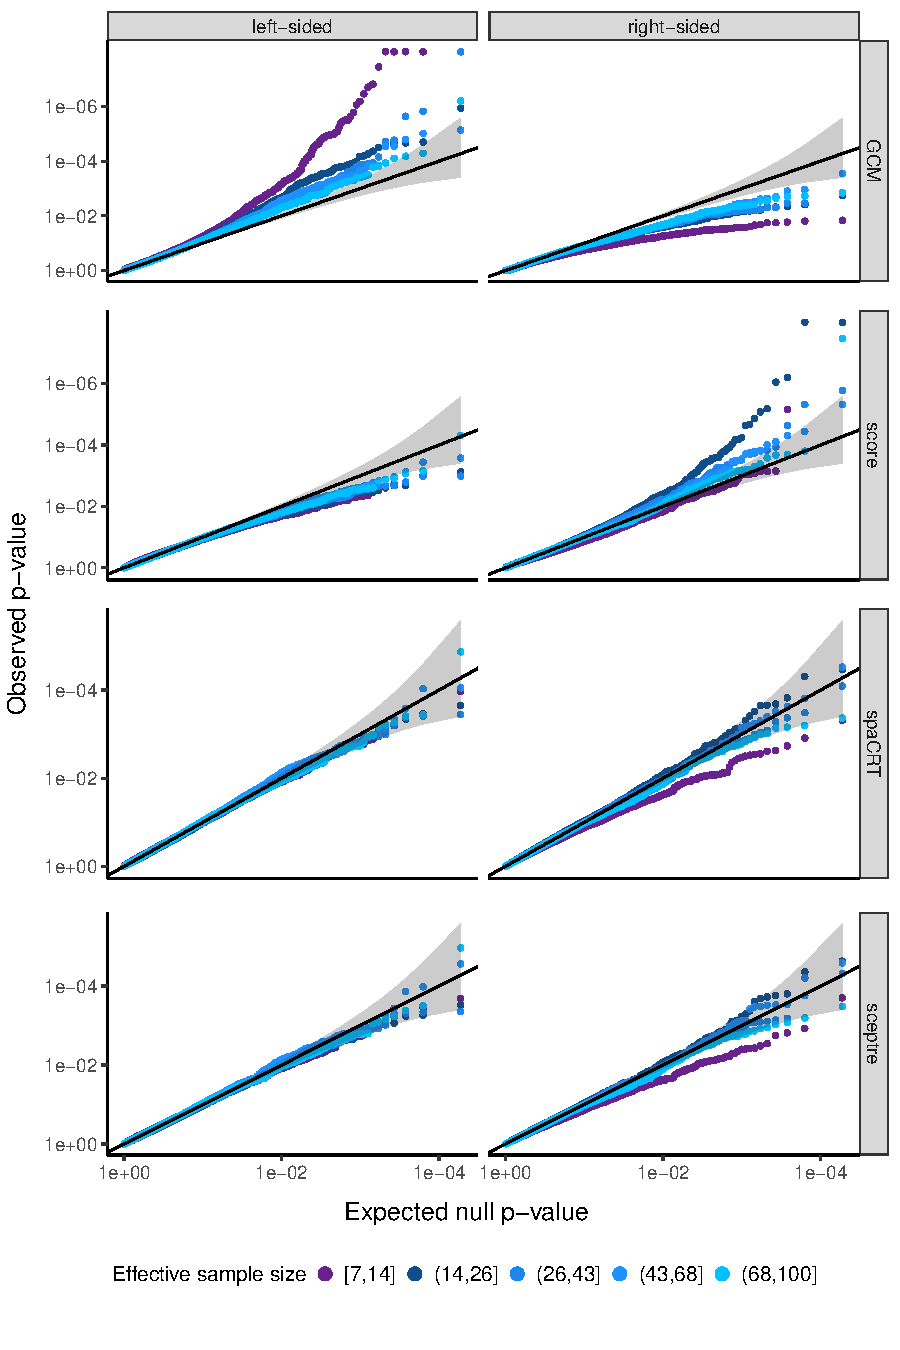
\includegraphics[width=0.9\textwidth]{figures-and-tables/facet_plot_different_withglmnb_100.pdf}
	\caption{QQ-plots for the $p$-values of right-sided test from different methods under low effective sample size.}
	\label{fig:qqplot_lowess}
\end{figure*}

\begin{figure*}[!ht]
	\centering
	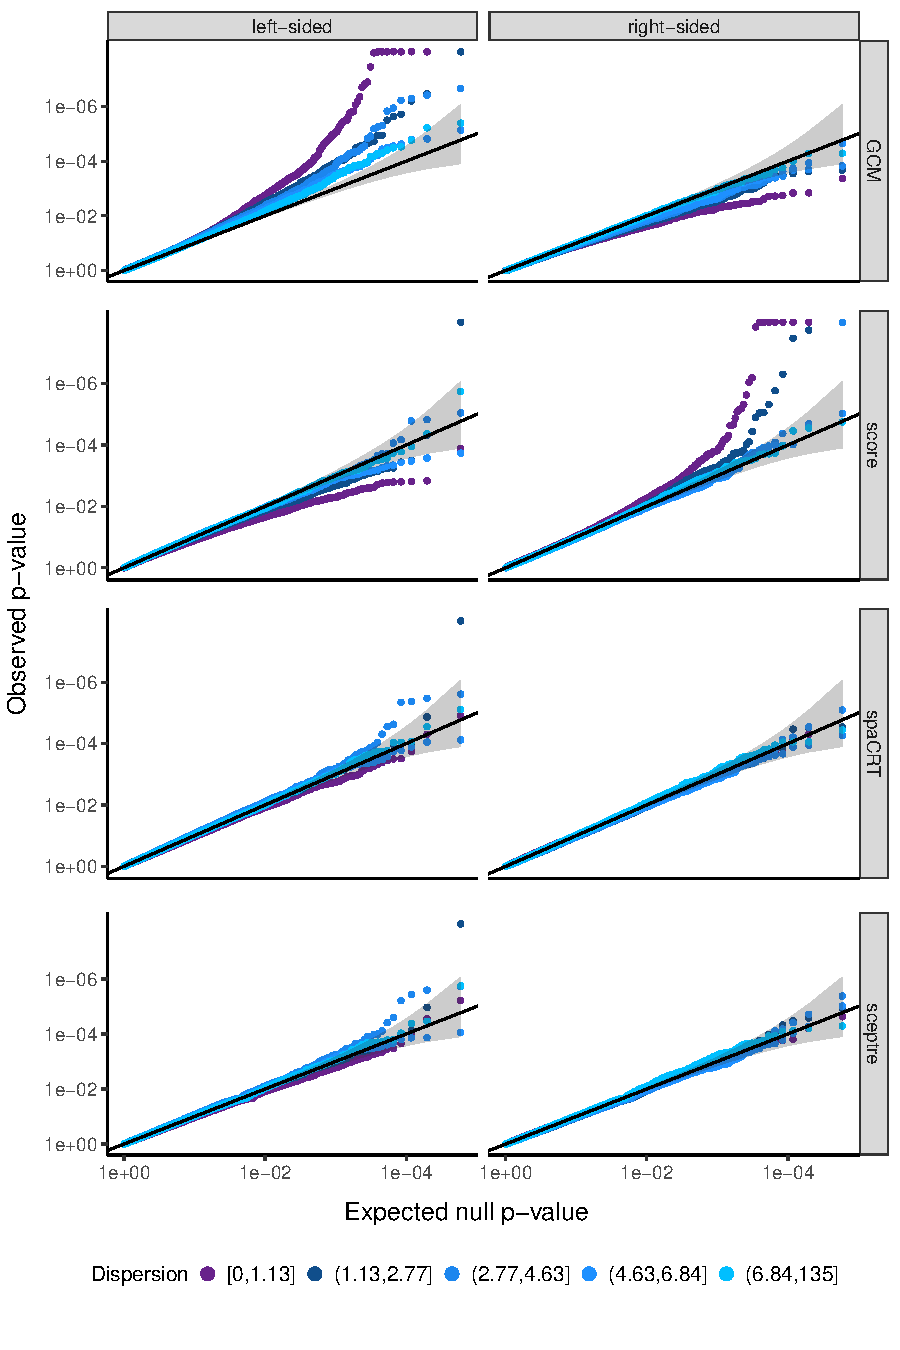
\includegraphics[width=0.9\textwidth]{figures-and-tables/facet_plot_different_withglmnb_dispersion.pdf}
	\caption{QQ-plots for the $p$-values of left-sided test from different methods stratified by dispersion parameter.}
	\label{fig:qqplot_dispersion}
\end{figure*}

\clearpage

\subsection{Additional tables for the real data analysis}\label{sec:additional_table_realdata}

\begin{table}[!h]
\centering
\caption{\label{tab:real_data_rejection}Number of rejections for negative control pairs on the Gasperini data.}
\centering
\begin{tabular}[t]{lrrrr}
\toprule
\multicolumn{1}{c}{ } & \multicolumn{4}{c}{Number of rejections} \\
\cmidrule(l{3pt}r{3pt}){2-5}
\multicolumn{1}{c}{ } & \multicolumn{2}{c}{Left-sided test} & \multicolumn{2}{c}{Right-sided test} \\
\cmidrule(l{3pt}r{3pt}){2-3} \cmidrule(l{3pt}r{3pt}){4-5}
\multicolumn{1}{c}{Method} & \multicolumn{1}{c}{Bonferroni} & \multicolumn{1}{c}{BH} & \multicolumn{1}{c}{Bonferroni} & \multicolumn{1}{c}{BH} \\
\cmidrule(l{3pt}r{3pt}){1-1} \cmidrule(l{3pt}r{3pt}){2-2} \cmidrule(l{3pt}r{3pt}){3-3} \cmidrule(l{3pt}r{3pt}){4-4} \cmidrule(l{3pt}r{3pt}){5-5}
GCM test & 22 & 128 & 0 & 0\\
Score test & 1 & 1 & 15 & 29\\
spaCRT & 1 & 1 & 0 & 0\\
dCRT & 1 & 4 & 0 & 0\\
\bottomrule
\end{tabular}
\end{table}



\end{document}






















 




